\documentclass[a4paper,11pt]{article}
\usepackage[a4paper,margin=2.5cm]{geometry}
\usepackage{amsmath,amsthm}
\usepackage{fontspec}
\usepackage{unicode-math}
\usepackage{graphicx}
\usepackage{booktabs}
\usepackage{tabularx}
\usepackage{xltabular}
\usepackage{xcolor}
\usepackage[hidelinks]{hyperref}
% ---------------------------------------------------------------------------
% Fonts (author's specification, 2026-11-25): Noto Sans for text, Noto Sans
% Math for mathematics, Fira Math as fallback for glyphs absent from Noto Sans
% Math. Fallback ranges are listed explicitly and were chosen from the build
% log ("Missing character" lines), not guessed.
% ---------------------------------------------------------------------------
\setmainfont{NotoSans}[Path=/usr/share/fonts/truetype/noto/,Extension=.ttf,
  UprightFont=*-Regular,BoldFont=*-Bold,ItalicFont=*-Italic,BoldItalicFont=*-BoldItalic]
\setsansfont{NotoSans}[Path=/usr/share/fonts/truetype/noto/,Extension=.ttf,
  UprightFont=*-Regular,BoldFont=*-Bold,ItalicFont=*-Italic,BoldItalicFont=*-BoldItalic]
\setmonofont{NotoSansMono}[Path=/usr/share/fonts/truetype/noto/,Extension=.ttf,UprightFont=*-Regular,Scale=0.92]
\setmathfont{NotoSansMath-Regular.otf}[Path=./fonts/]
% Fira Math fallback for glyphs absent from Noto Sans Math: none needed (build log has no Missing character).
\setlength{\emergencystretch}{2em}
\tracinglostchars=3 % any glyph missing from the loaded fonts is a hard error
\usepackage{newunicodechar}
\newunicodechar{ℤ}{$\mathbb{Z}$}
\setlength{\parskip}{0.45em}
\setlength{\parindent}{1.2em}
\setlength{\emergencystretch}{2em}
\tracinglostchars=3 % any glyph missing from the loaded fonts is a hard error
\numberwithin{equation}{section}
\newtheorem{proposition}{Proposition}[section]
\newtheorem{lemma}[proposition]{Lemma}
\theoremstyle{remark}
\newtheorem*{remark}{Remark}
% Epistemic label: rendered in small capitals, never in bold.
\newcommand{\lbl}[1]{\textsc{#1}.\ }
\newcommand{\grade}[1]{[\,#1\,]}
\newcommand{\Dfour}{D_4}

\begin{document}

\begin{titlepage}
\centering
\vspace*{2.5cm}
{\LARGE Intrinsic Resonance Holography}\\[0.8em]
{\Large Dynamical selection of a $D_4$ substrate from interference dynamics}\\[1.2em]
{\large Version 95 (draft of November 25, 2026)}\\[2.5em]
{\large Brandon D. McCrary}\\[0.4em]
Independent researcher\\[0.3em]
ORCID \href{https://orcid.org/0009-0008-2804-7165}{0009-0008-2804-7165}\\[2.5em]
\begin{minipage}{0.86\linewidth}
\small
This is a working draft of the ninety-fifth edition. It supersedes version 94 (November 14, 2026) as a statement of the programme, but version 94 remains the citable record of what was claimed on that date. Every change from version 94 is listed in Appendix~\ref{app:corrections} and in the accompanying change log. Verification data, scripts and the frozen pre-registrations referred to in the text are in the public repository \texttt{IRH-Theory-Development-Workspace} (GitHub account \texttt{brandonmccraryresearch-cloud}), under \texttt{programme/}.
\end{minipage}
\vfill
\end{titlepage}

\begin{abstract}
\noindent
We study a real scalar field $\psi$ on $\mathbb{R}^4$ whose free energy is the Swift--Hohenberg functional with a cubic and a quartic term, and ask which periodic pattern it forms when the uniform state becomes unstable. A Landau argument over the combinatorics of the reciprocal shell reduces the question to a single number for each candidate lattice, $S=\tau^2/q_4$, built from the counts $T$ of closed triads and $Q$ of closed quadruples among the $N$ shell vectors, normalised as $\tau=T/N^{3/2}$ and $q_4=Q/N^2$. The coupling constants drop out of the ordering. The same code reproduces the Alexander--McTague preference for bcc in three dimensions ($S=16/45$) and finds that in four dimensions the $D_4$ lattice wins, with $S_{D_4}=64/141$ against $S_{A_4^*}=12/31$, a margin of $73/423$. Simulations confirm that the cubic triad term is what decides the winner, that the symmetric 24-mode standing wave is an attractor of conserved dynamics, and that in the barrier-free part of the phase diagram a noise quench in a box of side $3\pi$ ends in a (generally rotated) $D_4$ root system in $29$ of $30$ runs. Selection from noise in general is not established. The $D_4$ phase occupies $758/6561\approx11.55\%$ of the standard parameter window, but only when the resonant wavenumber sits on the $D_4$ shell, and the transition into it is first order; the unrestricted critical droplet has excess free energy $119.06\pm0.03$, about $4.6$ times lower than the restricted-envelope saddle quoted in version 94.

Three results of the present edition bear on how the pattern could be read as spacetime. First, the Gaussian Swift--Hohenberg measure is not reflection positive: its propagator increases with $k^2$ below the shell, so it has no Källén--Lehmann representation, and the reflected kernel changes sign. Second, the long-wavelength phonons of the relaxed $D_4$ crystal form four gapless branches with exactly isotropic quadratic dispersion but two speeds, $c_L/c_T=1.731985$, within $10^{-4}$ of $\sqrt3$; we derive $c_L^2/c_T^2=3$ in closed form from a Cauchy relation that the shell geometry enforces, and show that an isotropic four-dimensional solid with a single sound speed would need a negative bulk modulus. Third, these two results remove the constructive routes of the two readings of the four-dimensional base that had been on the table, and under the rule fixed in advance the working reading becomes the one in which spacetime emerges from defect dynamics, a reading for which no construction yet exists. The algebraic sector is unchanged: $\mathfrak{so}(8)$ is excluded as a gauge algebra, the vertices of the 24-cell form the binary tetrahedral group whose McKay correspondent is affine $E_6$, and $E_6$ enters only as a label. Three generations of matter are an input. Every result carries an evidence grade, defined in Appendix~\ref{app:grades}, and no grade has been raised in this edition.
\end{abstract}

\tableofcontents
\clearpage

%===========================================================================
\section{Introduction}\label{sec:intro}
%===========================================================================

\subsection{The question}

Version 92 of this programme took the $D_4$ root lattice as a given four-dimensional scaffold and put fields on its sites. That formulation had three defects, all of which survived scrutiny. Its two ``primitive'' scales, the lattice spacing $a_0$ and the frequency $\Omega_P$, were defined through the Planck length as $a_0=L_P/\sqrt{24}$ and $\Omega_P=\sqrt{24}\,c/L_P$, with $L_P=\sqrt{\hbar G/c^3}$, so that the relations $c=a_0\Omega_P$, $\hbar=M^*ca_0$ and $G=24c^2a_0/M^*$, with $M^*$ the inertia carried by a lattice site, were a change of variables rather than a derivation. Nothing selected $D_4$ over $\mathbb{Z}^4$ or any other lattice; it was chosen because it fitted. And the discrete action mixed integer labels with dimensionful coordinates, writing shifts such as $\phi(n+a_0e_\mu)$ for $n\in\mathbb{Z}^4$, and stated two incompatible time steps.

The present formulation replaces the scaffold by a field. The primitive object is a real scalar $\psi(\mathbf{x},t)$ on $\mathbb{R}^4$, and $D_4$ is not assumed: it is the pattern of extrema into which $\psi$ organises itself when the uniform state becomes unstable. The question of the programme then becomes a question in pattern formation, and it can be asked precisely. Given a free energy that prefers wavevectors of one length, which periodic arrangement of those wavevectors does the field adopt, and is the answer stable, reachable from noise, and insensitive to the parameters?

This paper answers that question as far as the present evidence allows, and then asks what the answer could mean physically. The answer to the first question is largely affirmative and is reported in Sections~\ref{sec:substrate}--\ref{sec:nucleation}. The answer to the second is, at the time of writing, mostly negative, and Sections~\ref{sec:phonons}--\ref{sec:dimension} explain why.

\subsection{What is established and what is not}

Let us state the position at the outset, so that nothing later reads as a larger claim than it is.

The geometric and combinatorial core is solid. The 24 roots of $D_4$ form a spherical 5-design, so every quadratic and quartic moment is isotropic (Section~\ref{sec:geometry}); the selection criterion $S=\tau^2/q_4$ is derived symbolically and its values are exact rationals (Section~\ref{sec:selection}); these counts and the stability bound of the legacy discrete action are now theorems checked by the Lean~4 kernel (Section~\ref{sec:verification}). The causal role of the cubic term is shown by simulation, as is the dynamical stability of the full 24-mode state under conserved dynamics. The binary tetrahedral group, its McKay correspondent and the exclusion of $\mathfrak{so}(8)$ are exact algebra.

Several things are not established, and we say so where they arise. Selection of $D_4$ from generic noise has been shown only in a narrow barrier-free sliver of the phase diagram and in finite boxes (Sections~\ref{sec:selection} and \ref{sec:nucleation}). The $D_4$ phase exists only when the resonant wavenumber is tuned onto the shell. No mechanism fixes the baseline value $\bar\psi$ of the field. The rate at which the $D_4$ phase nucleates is not known. The identification of $E_6$ is a label: no Yang--Mills dynamics for an $E_6$ connection follows from the scalar dynamics. Three generations are not derived. And, as the new results of Sections~\ref{sec:rp}--\ref{sec:dimension} show, neither of the two concrete ways of reading the four-dimensional base as spacetime survives: the Euclidean reading has no reflection-positive Gaussian measure, and the reading with four spatial dimensions and one compactified produces two light cones.

\subsection{How the paper is organised, and how claims are graded}

Section~\ref{sec:substrate} defines the field, the functional and the three dynamics we use. Section~\ref{sec:geometry} collects the geometry of $D_4$ that the rest of the paper needs. Sections~\ref{sec:selection} and \ref{sec:band} derive the selection criterion, test it, and map the region of parameters where $D_4$ is the ground state. Section~\ref{sec:stability} treats the stability of the ordered state and Section~\ref{sec:nucleation} the first-order transition into it. Section~\ref{sec:phonons} computes the elastic constants and phonon spectrum of the crystal. Section~\ref{sec:legacy} keeps, with its scope stated, the discrete site-field action of the earlier versions, and Section~\ref{sec:four} gives the scaling argument for four dimensions. Sections~\ref{sec:algebra} and \ref{sec:defects} treat the algebraic sector and the defects. Section~\ref{sec:rp} is new and concerns reflection positivity; Section~\ref{sec:dimension} brings the phonon and positivity results to bear on the dimensional assignment. Section~\ref{sec:predictions} lists what the framework predicts, Section~\ref{sec:verification} what has been checked independently and formally, Section~\ref{sec:retractions} what has been withdrawn, and Sections~\ref{sec:status}--\ref{sec:assessment} give the status of every gap and our assessment. Appendix~\ref{app:corrections} records every correction, Appendix~\ref{app:methods} the methods, tools and grading rules.

Each claim carries one of six epistemic labels, set in small capitals. A \lbl{Derivation} follows from stated assumptions without empirical input. A \lbl{Prediction} is an output of the model that does not depend on the data it would be compared with. A \lbl{Calibration} is a parameter adjusted to fit data and is never presented as a prediction. An \lbl{Input} is an assumption, acknowledged as such. An \lbl{Exclusion} is a result ruled out by proof. An \lbl{Open} item is a well-posed question not settled here. In addition, results carry an evidence grade in square brackets, for example \grade{B, F2/I1}. The letter (A to D) measures how strong the evidence is, the F-level (F1 to F3) how a computational result was reproduced, and the I-level (I0 to I4) how independent the checks were of the person or system that produced the result. Appendix~\ref{app:grades} defines these levels exactly. One feature of them matters throughout: every computational check reported here was produced and verified by tools run under the author's direction, so independence never exceeds I1, and no grade in this paper should be read as external confirmation. Labels of the form G-A5 or G-D3 name entries of the programme's gap inventory, which is kept with the repository records; a run number, such as run 13, names one verification cycle of the programme.

% NOTATION-TABLE-BEGIN
\subsection{Notation}\label{sec:notation}

Table~\ref{tab:notation} lists the symbols used in more than one section, with the place where each is defined. A few letters carry a second, local meaning in one section only, and the table says where; in each such place the meaning is restated.

\begin{table}[htbp]
\centering
\small
\begin{tabular}{p{0.2\linewidth}p{0.5\linewidth}p{0.2\linewidth}}
\toprule
symbol & meaning & defined in\\
\midrule
$\psi$, $\bar\psi$, $\varphi$ & tension field; its spatial mean (baseline tension); its deviation $\psi-\bar\psi$ & Sections~\ref{sec:substrate}, \ref{sec:band}\\
$F$, $r$, $q_0$, $u$, $v$ & free energy; quench depth; resonant wavenumber; cubic and quartic couplings & \eqref{eq:F}\\
$\gamma$ & damping of the wave equation & \eqref{eq:dw}\\
$a_0$ & spatial period of the pattern, $2\pi/q_0$ & \eqref{eq:a0}\\
$\Phi$, $D_4$, $D_4^*$ & root system of $D_4$; the root lattice; its dual & Section~\ref{sec:geometry}\\
$N$, $T$, $Q$ & number of shell vectors; ordered closed triads; ordered closed quadruples & Section~\ref{sec:selection}\\
$\tau$, $q_4$, $S$ & normalised counts $T/N^{3/2}$, $Q/N^2$; selection ratio $\tau^2/q_4$ & \eqref{eq:FB}, \eqref{eq:S}\\
$A$, $B$ & per-mode amplitude; normalised amplitude $A\sqrt N$ & Section~\ref{sec:selection}\\
$F_{\rm exc}$, $r_{\rm eff}$, $u_{\rm eff}$ & excess over the uniform state; effective quadratic and cubic coefficients & \eqref{eq:Fmod}\\
$L$ & side of the periodic simulation box & Section~\ref{sec:sim}\\
$C_{ijkl}$, $\lambda$, $\mu$, $\rho$, $K$ & elastic tensor; Lamé constants; mass density; bulk modulus & Section~\ref{sec:phonons}\\
$c_L$, $c_T$ & longitudinal and transverse sound speeds & \eqref{eq:speeds}\\
$W(D_4)$, $W(F_4)$ & Weyl group of $D_4$; point group of the $D_4$ lattice & Sections~\ref{sec:algebra}, \ref{sec:defects}\\
$2T$, $Q_8$ & binary tetrahedral group; quaternion group & Section~\ref{sec:algebra}\\
\bottomrule
\end{tabular}
\caption{Notation. Local second meanings: in simulation statements $N$ is also the number of grid points per side; in Section~\ref{sec:legacy} $\phi$ is the site field, $\mu^2$ a mass parameter, $J$ a coupling and $\theta$ a carrier angle; in Section~\ref{sec:nucleation} $J$ is a rate prefactor; in Section~\ref{sec:rp} $\theta$ is a reflection; $\lambda$ also denotes a Hessian eigenvalue, and in Section~\ref{sec:four} a scale factor.}
\label{tab:notation}
\end{table}
% NOTATION-TABLE-END

%===========================================================================
\section{The substrate and its dynamics}\label{sec:substrate}
%===========================================================================

\subsection{The free energy}

Let $\psi:\mathbb{R}^4\to\mathbb{R}$ be a real field, which we call the tension field. Its free energy is
\begin{equation}\label{eq:F}
F[\psi]=\int d^4x\;\Big[\tfrac12\,\psi\,\big(r+(q_0^2+\nabla^2)^2\big)\,\psi-\tfrac{u}{3}\,\psi^3+\tfrac{v}{4}\,\psi^4\Big].
\end{equation}
Here $\nabla^2=\sum_{i=1}^4\partial_i^2$ is the Laplacian, $q_0>0$ is a wavenumber, $r$ is a real parameter we call the quench depth, and $u,v>0$ are the cubic and quartic couplings. The operator $(q_0^2+\nabla^2)^2$ is the one introduced by Swift and Hohenberg~\cite{ref2}. Acting on a plane wave $e^{i\mathbf{k}\cdot\mathbf{x}}$ it gives $(q_0^2-|\mathbf{k}|^2)^2e^{i\mathbf{k}\cdot\mathbf{x}}$, because $\nabla^2e^{i\mathbf{k}\cdot\mathbf{x}}=-|\mathbf{k}|^2e^{i\mathbf{k}\cdot\mathbf{x}}$. So the quadratic part of $F$ costs nothing extra for wavevectors on the sphere $|\mathbf{k}|=q_0$, which we call the resonant shell, and penalises every other wavevector by the square of its distance from the shell in $|\mathbf{k}|^2$. When $r<0$ the modes on the shell lower the energy and the uniform state $\psi=0$ is unstable.

The functional derivative of $F$, which drives all the dynamics below, follows from varying $\psi\to\psi+\delta\psi$ and integrating by parts twice (the operator $(q_0^2+\nabla^2)^2$ is self-adjoint on periodic or decaying fields):
\begin{equation}\label{eq:dF}
\frac{\delta F}{\delta\psi}=\big(r+(q_0^2+\nabla^2)^2\big)\psi-u\,\psi^2+v\,\psi^3 .
\end{equation}

\subsection{Three dynamics}

We use three evolution laws built on the functional derivative \eqref{eq:dF}, and it matters which is used where.

The first is a damped wave equation,
\begin{equation}\label{eq:dw}
\partial_t^2\psi+\gamma\,\partial_t\psi=-\frac{\delta F}{\delta\psi},
\end{equation}
with damping $\gamma>0$. The second-order term carries the tension of the substrate and the first-order term its relaxation. This is the law integrated for the noise quenches of Section~\ref{sec:sim}. The second is non-conserved relaxation, Model~A in the classification of Hohenberg and Halperin~\cite{ref4},
\begin{equation}\label{eq:A}
\partial_t\psi=-\frac{\delta F}{\delta\psi},
\end{equation}
and the third is conserved relaxation, Model~B~\cite{ref4},
\begin{equation}\label{eq:B}
\partial_t\psi=\nabla^2\frac{\delta F}{\delta\psi}.
\end{equation}
Model~B conserves the spatial mean $\bar\psi=V^{-1}\int\psi\,d^4x$ on a periodic box of volume $V$, because the right-hand side is a divergence and integrates to zero. The attractor tests of Section~\ref{sec:stability} and the selection tests of Section~\ref{sec:gd3} use Model~B. The inertial and conserved law $\partial_t^2\psi+\gamma\partial_t\psi=\nabla^2(\delta F/\delta\psi)$, which is the modified phase-field-crystal equation of Stefanovic, Haataja and Provatas~\cite{ref46}, joins the two features we need; it conserves $\bar\psi$ when the initial $\partial_t\psi$ has zero mean. We record it as the natural generalisation, but no result in this paper was obtained by integrating it, apart from one verifier-side check in Section~\ref{sec:phonons}.

\subsection{First consequences}

\lbl{Derivation} The lattice constant is an output. A pattern built from wavevectors on the shell $|\mathbf{k}|=q_0$ has spatial period
\begin{equation}\label{eq:a0}
a_0=\frac{2\pi}{q_0}.
\end{equation}
This is not the old circularity in new symbols. In version 92, $a_0$ was defined through $L_P$. Here it is fixed by the dispersion of the substrate, and the objection to it as a primitive disappears rather than being patched.

\lbl{Derivation} The site-field action is retired. A field defined at the sites of a lattice presupposes the static picture. In the present picture the sites are the loci where $|\psi|$ is extremal; they carry no degrees of freedom of their own. The results derived from the site-field action (an exact dispersion relation and a stability bound) remain correct for that formulation and are kept in Section~\ref{sec:legacy}, with that scope.

\lbl{Derivation} The substrate needs conserved dynamics. Under Model~A the mean field is not protected; in a numerical run it drifts by $1.8\times10^{-1}$, while under Model~B it is preserved to $8.3\times10^{-17}$, which is round-off. Section~\ref{sec:band} shows that the full $D_4$ pattern is the ground state only in a band of $\bar\psi$, and Model~A carries $\bar\psi$ out of that band. So if the $D_4$ pattern is to persist, the total tension $\int\psi$ must be a conserved quantity. We treat conservation as a requirement of the framework and list it among the inputs.

%===========================================================================
\section{Geometry of $D_4$}\label{sec:geometry}
%===========================================================================

\subsection{Roots, shells and designs}

The $D_4$ root system is the set
\[
\Phi=\{\pm e_i\pm e_j:\ 1\le i<j\le4\}\subset\mathbb{R}^4,
\]
where $e_1,\dots,e_4$ is the standard basis. Choosing the pair $\{i,j\}$ in $\binom42=6$ ways and the two signs in $4$ ways gives $|\Phi|=24$ vectors, each of squared length $2$. The $D_4$ lattice is the integer span of $\Phi$, equivalently the set of integer vectors with even coordinate sum. Its dual lattice $D_4^*$ consists of the vectors $\mathbf{y}$ with $\mathbf{y}\cdot\mathbf{x}\in\mathbb{Z}$ for all $\mathbf{x}\in D_4$; it is $\mathbb{Z}^4\cup(\mathbb{Z}^4+\tfrac12(1,1,1,1))$. Its shortest nonzero vectors are the 8 vectors $\pm e_i$ and the 16 vectors $\tfrac12(\pm1,\pm1,\pm1,\pm1)$, all of length $1$. These 24 vectors have the same pairwise cosines, $\{-1,-\tfrac12,0,\tfrac12\}$, as the 24 roots: $D_4$ is isodual, congruent to its own dual up to scale and rotation~\cite{ref6}.

A finite set $X$ on a sphere is a spherical $t$-design if the average over $X$ of every polynomial of degree at most $t$ equals its average over the sphere~\cite{ref5}. The normalised roots of $D_4$ form a 5-design, and no set of 24 points on $S^3$ forms a 6-design~\cite{ref5}.

\subsection{Isotropy through fourth order}

\lbl{Derivation} For every $\mathbf{k}\in\mathbb{R}^4$,
\begin{equation}\label{eq:moments}
\sum_{\alpha\in\Phi}(\mathbf{k}\cdot\alpha)^2=12\,|\mathbf{k}|^2,\qquad
\sum_{\alpha\in\Phi}(\mathbf{k}\cdot\alpha)^4=12\,|\mathbf{k}|^4 .
\end{equation}
The computation goes pair by pair. For a fixed pair $\{i,j\}$ the four roots contribute $\mathbf{k}\cdot\alpha=\pm k_i\pm k_j$. At second order,
\[
(k_i+k_j)^2+(k_i-k_j)^2+(-k_i+k_j)^2+(-k_i-k_j)^2=4k_i^2+4k_j^2,
\]
since the cross terms cancel in pairs. At fourth order, expanding $(k_i\pm k_j)^4=k_i^4\pm4k_i^3k_j+6k_i^2k_j^2\pm4k_ik_j^3+k_j^4$ and adding the four sign choices, the odd terms cancel and we obtain $4k_i^4+24k_i^2k_j^2+4k_j^4$. Each index $i$ belongs to three of the six pairs. Summing over pairs therefore gives $12\sum_ik_i^2=12|\mathbf{k}|^2$ at second order, and
\[
12\sum_ik_i^4+24\sum_{i<j}k_i^2k_j^2=12\Big(\sum_ik_i^2\Big)^2=12|\mathbf{k}|^4
\]
at fourth order. Both identities hold with zero residual in SymPy~1.14.0 and Singular~4.4.1, and they are kernel-checked theorems in Lean (Section~\ref{sec:verification}). They are not accidents: they are the 5-design property applied to $(\mathbf{k}\cdot\hat\alpha)^2$ and $(\mathbf{k}\cdot\hat\alpha)^4$. The first directional dependence appears at sixth order.

Figure~\ref{fig:moment} contrasts this with the eight vectors $\pm e_i$ of the hypercubic lattice, whose fourth moment varies by $32\%$ over directions. The anisotropy coefficient $\xi_2=-1/384$ stated in version 92 was computed for that hypercubic stand-in, not for $D_4$, and is withdrawn (Section~\ref{sec:retractions}).

\begin{figure}[htbp]
\centering
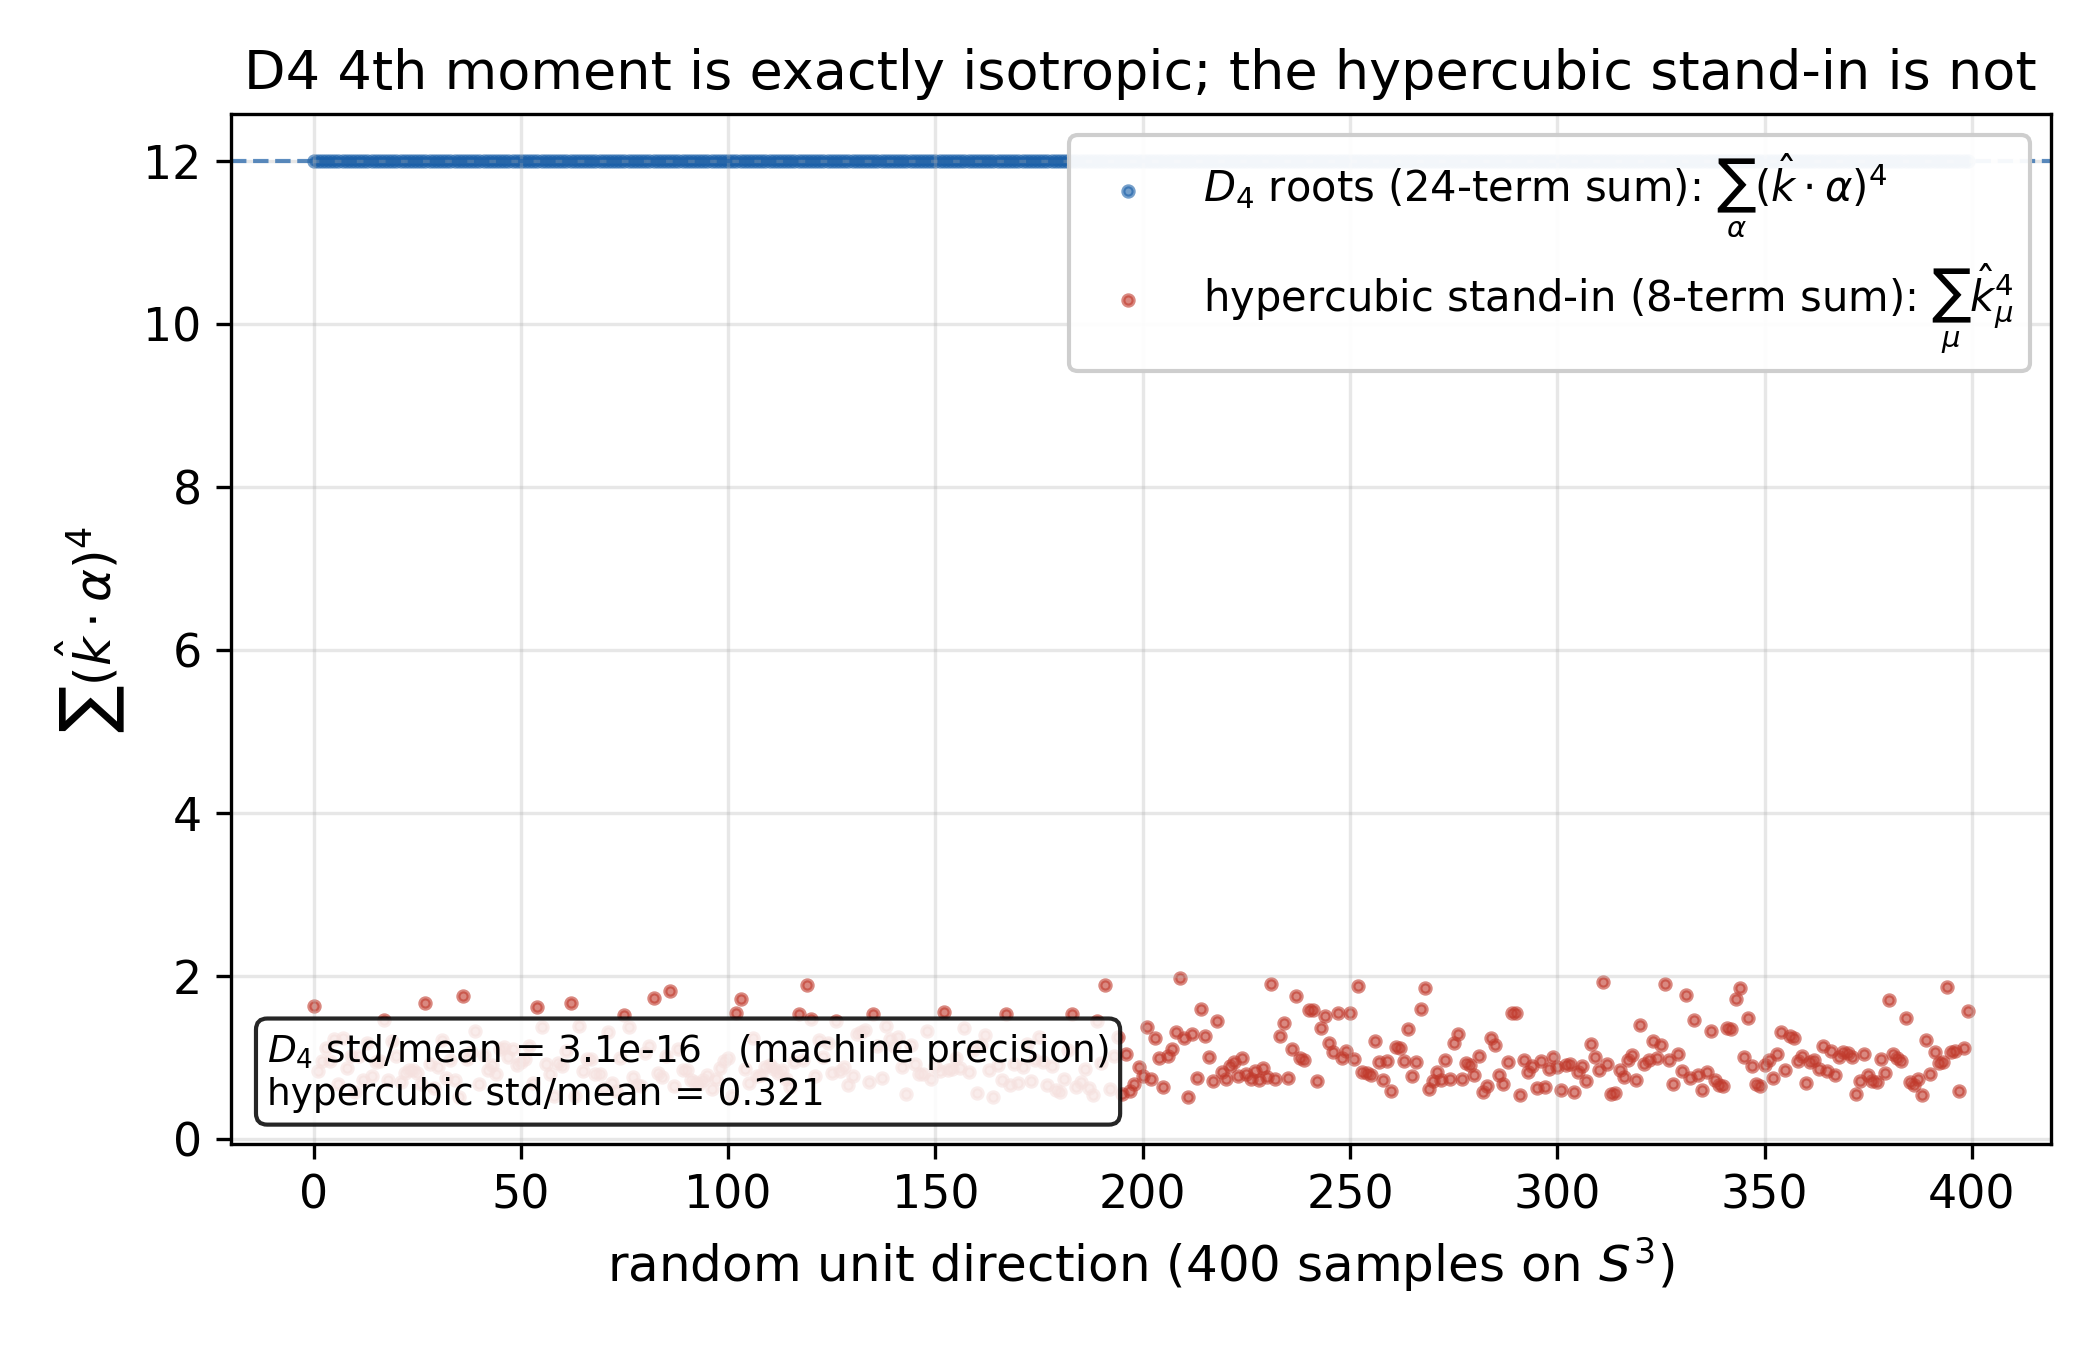
\includegraphics[width=0.85\linewidth]{figs/fig02.png}
\caption{The fourth moment $\sum_\alpha(\hat{\mathbf{k}}\cdot\alpha)^4$ at 400 random directions $\hat{\mathbf{k}}\in S^3$, for the 24 roots of $D_4$ and for the 8 vectors $\pm e_i$ of $\mathbb{Z}^4$. The $D_4$ sum is constant to machine precision; the hypercubic sum varies by $32\%$.}
\label{fig:moment}
\end{figure}

\subsection{Interference maxima}

The informal picture of the substrate as a resonant cavity becomes a reciprocal-lattice problem: which superposition of plane waves interferes constructively exactly at the points of $D_4$? Put the field on the torus $\mathbb{R}^4/\Lambda$ with $\Lambda\cong D_4$. Then the allowed wavevectors are those of the dual lattice, and the shortest of them form the reciprocal shell. By isoduality this shell is congruent to $\Phi$ itself. Form
\begin{equation}\label{eq:Psi}
\Psi(\mathbf{x})=\sum_{\mathbf{g}}\cos(2\pi\,\mathbf{g}\cdot\mathbf{x}),
\end{equation}
the sum running over the 24 shortest vectors $\mathbf{g}$ of $D_4^*$. At a point of $D_4$ every $\mathbf{g}\cdot\mathbf{x}$ is an integer, so every cosine is $1$ and $\Psi=24$. An exhaustive scan of $25^4=390{,}625$ points of a fundamental domain finds $\Psi=24$ only at the lattice point, $\Psi=-8$ at the nearest point of $\mathbb{Z}^4$ outside $D_4$ and at the deep hole $(\tfrac12,\tfrac12,\tfrac12,\tfrac12)$, and no other point within $0.1\%$ of the maximum.

The maximum is unique modulo the lattice, and only in that sense. On a periodic grid it recurs at every image. A grid of $16^4$ points carrying two periods of the pattern in each direction contains $2^4=16$ copies of the fundamental cell, and the checkerboard structure of $D_4$ gives two maxima per copy (the corner and body-centre families), so the maximum is attained at $32$ grid points. The exact maximum set on that grid is a kernel-checked theorem (claim C16 of Section~\ref{sec:verification}); the $0.1\%$ margin is a floating-point statement.

Isoduality alone does not select $D_4$: the hypercubic lattice is also isodual and resonates with itself by the same argument, since every $\mathbf{g}\cdot\mathbf{x}$ is an integer at its own lattice points. Selection needs the nonlinear terms of the free energy \eqref{eq:F}, to which we now turn.

\subsection{Cross-section and optimality}

\lbl{Derivation} The hyperplane $x_4=0$ meets $D_4$ in the integer vectors of $\mathbb{R}^3$ with even coordinate sum, which is the face-centred cubic lattice $D_3$, of kissing number 12, the densest lattice packing in three dimensions~\cite{ref6}.

The lattice $D_4$ is the unique optimal kissing configuration in four dimensions~\cite{ref7}, but it is not universally optimal in the sense of Cohn and Kumar~\cite{ref43}, that is, it does not minimise every completely monotonic pair potential~\cite{ref13}. A random-restart minimisation over the Gaussian family $e^{-\beta|x-y|^2}$, which by Bernstein's theorem~\cite{ref12} generates the completely monotonic class, recovers $D_4$ as the optimum to about $10^{-13}$ relative accuracy for $\beta\in[0.05,2.4]\cup[3.1,12]$ and finds a lower-symmetry configuration that wins by at most $0.007\%$ for $\beta\in[2.6,3.0]$; see also~\cite{ref14}. The claim we make is therefore narrower: $D_4$ minimises the particular triad-reinforcing functional relevant to standing-wave selection.

A broader claim made in version 93.1, that this programme alone occupies the corner of a classification of selection principles labelled (2,2), does not hold under its own definition: two other published models score (2,2,2) and (2,1,1) \grade{B}. Narrowed to purely spectral (Turing-type) selection, no retrieved approach occupies that corner \grade{C}; we do not evaluate the physics of the rival models (gap G-D10).

%===========================================================================
\section{The selection criterion}\label{sec:selection}
%===========================================================================

\subsection{Reduction to shell combinatorics}

Suppose the field orders on a single shell of $N$ wavevectors $\mathbf{g}_1,\dots,\mathbf{g}_N$, closed under $\mathbf{g}\mapsto-\mathbf{g}$ and lying exactly on the resonant sphere, so that the operator $(q_0^2+\nabla^2)^2$ annihilates each mode. Take all amplitudes equal and in phase,
\[
\psi(\mathbf{x})=A\sum_{a=1}^{N}e^{i\mathbf{g}_a\cdot\mathbf{x}},
\]
which is real because the shell is closed under negation. The spatial average of a product of plane waves $e^{i(\mathbf{g}_{a_1}+\dots+\mathbf{g}_{a_m})\cdot\mathbf{x}}$ is $1$ if the wavevectors sum to zero and $0$ otherwise. Hence $\langle\psi^m\rangle=A^m\,\#\{(a_1,\dots,a_m):\mathbf{g}_{a_1}+\dots+\mathbf{g}_{a_m}=0\}$. For $m=2$ the count is $N$ (each $\mathbf{g}$ with $-\mathbf{g}$). Write $T$ for the count at $m=3$, the number of ordered closed triads, and $Q$ for the count at $m=4$, the number of ordered closed quadruples. Because each mode is annihilated by $(q_0^2+\nabla^2)^2$, the quadratic term of the free energy \eqref{eq:F} reduces to $\tfrac r2\langle\psi^2\rangle$, and averaging the integrand over the volume $V$ gives the free-energy density
\begin{equation}\label{eq:Fshell}
\frac{F}{V}=\frac r2\,NA^2-\frac u3\,TA^3+\frac v4\,QA^4 .
\end{equation}
In the normalised amplitude $B=A\sqrt N$ the three powers are $NA^2=B^2$, $TA^3=(T/N^{3/2})B^3$ and $QA^4=(Q/N^2)B^4$, so
\begin{equation}\label{eq:FB}
f(B)=\frac r2B^2-\frac u3\,\tau B^3+\frac v4\,q_4B^4,\qquad \tau\equiv\frac{T}{N^{3/2}},\quad q_4\equiv\frac{Q}{N^2}.
\end{equation}

\subsection{The first-order point}

The ordered state becomes degenerate with the uniform state when $f$ has a nonzero critical point at height zero, $f(B)=0$ and $f'(B)=0$ with $B\ne0$. We solve these two conditions for $B$ and $r$ by eliminating $r$ between them. Dividing $f'(B)=0$ by $B$ gives
\[
r-u\tau B+vq_4B^2=0,
\]
and dividing $f(B)=0$ by $B^2$ and multiplying by $2$ gives
\[
r-\tfrac23u\tau B+\tfrac12vq_4B^2=0 .
\]
Subtracting the second equation from the first leaves $-\tfrac13u\tau B+\tfrac12vq_4B^2=0$, so
\[
B_*=\frac{2u\tau}{3vq_4}.
\]
Substituting into the first equation, $r_c=u\tau B_*-vq_4B_*^2=\frac{2u^2\tau^2}{3vq_4}-\frac{4u^2\tau^2}{9vq_4}$, that is,
\begin{equation}\label{eq:rc}
r_c=\frac29\,\frac{u^2}{v}\,\frac{\tau^2}{q_4}.
\end{equation}
\lbl{Derivation} The pattern that orders first, at the largest $r_c$ and hence the shallowest quench, is the one that maximises
\begin{equation}\label{eq:S}
S=\frac{\tau^2}{q_4}.
\end{equation}
The couplings enter \eqref{eq:rc} only through the common factor $2u^2/(9v)$, so they rescale $r_c$ but cannot change the order of the candidates. Selection depends on the shell alone. A shell without closed triads has $T=0$, hence $S=0$, and cannot order through the cubic mechanism at all.

The quantity $\tau$ here counts closed triads on a reciprocal shell. It has nothing to do with the time-like parameter $\tau$ of Perelman's entropy functionals, and $S$ is a ratio of combinatorial counts, not an entropy.

\subsection{Three dimensions}

Before using \eqref{eq:S} in four dimensions we require it to reproduce the known three-dimensional answer. For bcc the reciprocal shell has $N=12$ vectors and $T=48$, so
\[
\tau=\frac{48}{12^{3/2}}=\frac{48}{12\cdot2\sqrt3}=\frac{2}{\sqrt3},\qquad \tau^2=\frac43 .
\]
With $Q=540$ we get $q_4=540/144=15/4$ and $S=(4/3)/(15/4)=16/45\approx0.35556$. For fcc ($N=8$, $Q=216$, $q_4=27/8$) and simple cubic ($N=6$, $Q=90$, $q_4=5/2$) there are no closed triads, $T=0$, and $S=0$. The criterion selects bcc, which is the Alexander--McTague result~\cite{ref1}, recovered by the same code that is used below in four dimensions. That result holds near melting; Groh and Mulder showed that away from that regime the liquid--solid transition need not produce bcc~\cite{ref44}, and the criterion inherits the same domain of validity.

\subsection{Four dimensions}

\lbl{Prediction} Table~\ref{tab:S4} gives the four candidates. Rows are labelled by the crystal, and $N$ is the size of that crystal's reciprocal minimal shell, because the density is expanded in reciprocal vectors; so the $A_4^*$ row shows the $A_4$ shell ($N=20$) and the $A_4$ row the $A_4^*$ shell ($N=10$).

\begin{table}[htbp]
\centering
\begin{tabular}{lrrrrrr}
\toprule
crystal & $N$ & $T$ & $Q$ & $\tau^2$ & $q_4$ & $S=\tau^2/q_4$\\
\midrule
$D_4$ & 24 & 192 & 3384 & $8/3$ & $47/8$ & $64/141\approx0.453901$\\
$A_4^*$ & 20 & 120 & 1860 & $9/5$ & $93/20$ & $12/31\approx0.387097$\\
$\mathbb{Z}^4$ & 8 & 0 & 168 & $0$ & $21/8$ & $0$\\
$A_4$ & 10 & 0 & 270 & $0$ & $27/10$ & $0$\\
\bottomrule
\end{tabular}
\caption{The selection criterion in four dimensions. All entries are exact.}
\label{tab:S4}
\end{table}

For $D_4$, $\tau=192/24^{3/2}=192/(24\cdot2\sqrt6)=4/\sqrt6$, so $\tau^2=8/3$; and $q_4=3384/576=47/8$ after dividing numerator and denominator by $72$. Then $S=(8/3)(8/47)=64/141$. For $A_4^*$, $\tau=120/20^{3/2}=3/\sqrt5$, $\tau^2=9/5$, $q_4=1860/400=93/20$, and $S=(9/5)(20/93)=12/31$. The ratio is
\[
\frac{S_{D_4}}{S_{A_4^*}}=\frac{64}{141}\cdot\frac{31}{12}=\frac{1984}{1692}=\frac{496}{423},
\]
a margin of $73/423\approx17.26\%$. The ratio of triad densities to bcc is $\tau_{D_4}/\tau_{\rm bcc}=(4/\sqrt6)(\sqrt3/2)=\sqrt2$ exactly. So $D_4$ is the four-dimensional analogue of bcc, and a stronger one. The counts $T$ and $Q$ for $D_4$ and $A_4^*$, the four values of $S$ and the ratio $496/423$ are kernel-checked theorems (claims C01--C10 of Section~\ref{sec:verification}).

The triad count has a geometric reading that connects this section to the interference picture. Each root $\alpha\in\Phi$ has exactly $8$ roots $\beta$ with $\alpha\cdot\beta=-1$, that is, at $120^\circ$, and for each such $\beta$ the vector $-\alpha-\beta$ is again a root. So the closed triads are counted by $24\times8=192=T$. The vectors that interfere constructively at the lattice points and the vectors whose triads lower the energy are the same 24 vectors.

The analytic prediction agrees with a molecular-dynamics study, by an entirely different method, in which supercooled four-dimensional Lennard-Jones liquids crystallise into $D_4$ rather than $A_4$~\cite{ref40}; at zero pressure and reduced temperature $T^*$ with $0.59<T^*<0.63$ the liquid crystallises within about $2\times10^4$ time units, and $N=648$ atoms, eight per unit cell, give a $3\times3\times3\times3$-cell single crystal. Freezing of four-dimensional hard spheres is also consistent with $D_4$ symmetry~\cite{ref39}. In the equilibrium Landau setting, Elitzur, Karni and Rabinovici showed that in four dimensions the cubic term is maximised by the cross-polytope, whose reciprocal lattice is $D_4$~\cite{ref45}. Their argument is static and ours is dynamical; they select the same winner.

\subsection{Selection in simulation: the causal test}\label{sec:sim}

Minimising a functional and reaching the minimum dynamically are different statements, and the second has to be tested.

We integrate the damped wave equation \eqref{eq:dw} on a periodic $16^4$ grid with a semi-implicit pseudo-spectral scheme~\cite{ref10}, treating the linear operator implicitly in Fourier space. The box has side $L=2\pi$, so the allowed wavevectors are integer vectors $\mathbf{n}$. The $D_4$ shell is then the scaled root set $\{(\pm2,\pm2,0,0)$ and permutations$\}$, of squared length $8$; it fits two periods of the pattern in each direction. (A reader using roots of squared length $2$ rescales; the configuration is the same.) We set $q_0^2=7.5$, which places two integer shells at equal distance from resonance, as Table~\ref{tab:compet} shows.

\begin{table}[htbp]
\centering
\begin{tabular}{lrrrr}
\toprule
shell & $|\mathbf{k}|^2$ & modes & $T$ & penalty $(q_0^2-|\mathbf{k}|^2)^2$\\
\midrule
$D_4$ star $(\pm2,\pm2,0,0)$ & 8 & 24 & 192 & 0.25\\
competitor $(\pm2,\pm1,\pm1,\pm1)$ & 7 & 64 & 0 & 0.25\\
\bottomrule
\end{tabular}
\caption{The two shells in the causal test at $q_0^2=7.5$.}
\label{tab:compet}
\end{table}

The competitor has $4\times2^4=64$ modes (four positions for the entry $\pm2$, sixteen sign choices), about $2.7$ times as many as $D_4$, and no closed triads. The two linear penalties are $(7.5-8)^2=(7.5-7)^2=0.25$, so the linear growth rates are exactly equal and only the cubic term can break the tie. The other parameters are $r=-0.35$, $u=v=1$, $\gamma=1.2$, $\Delta t=0.05$: $6000$ steps for a direct quench, and for the annealed run a ramp of $r$ from $-0.05$ to $-0.45$ over $14000$ steps with decaying stochastic forcing.

In the author's run the $D_4$ shell took $84\%$ of the spectral power on direct quench and $100\%$ after annealing. With the cubic coupling set to zero the split was $44\%$ against $56\%$. An independent implementation with different seeds (random initial field of standard deviation $0.05$, annealing noise $0.5$ decaying linearly) found $77.1\%$ on $D_4$ with triads and $21.1\%$ without, rising to $89.5\%$ under annealing and still increasing at step $14000$. The exact shares depend on the implementation. The conclusion does not: switching off the triad term reverses the winner. These are power shares, not recovery rates.

\begin{figure}[htbp]
\centering
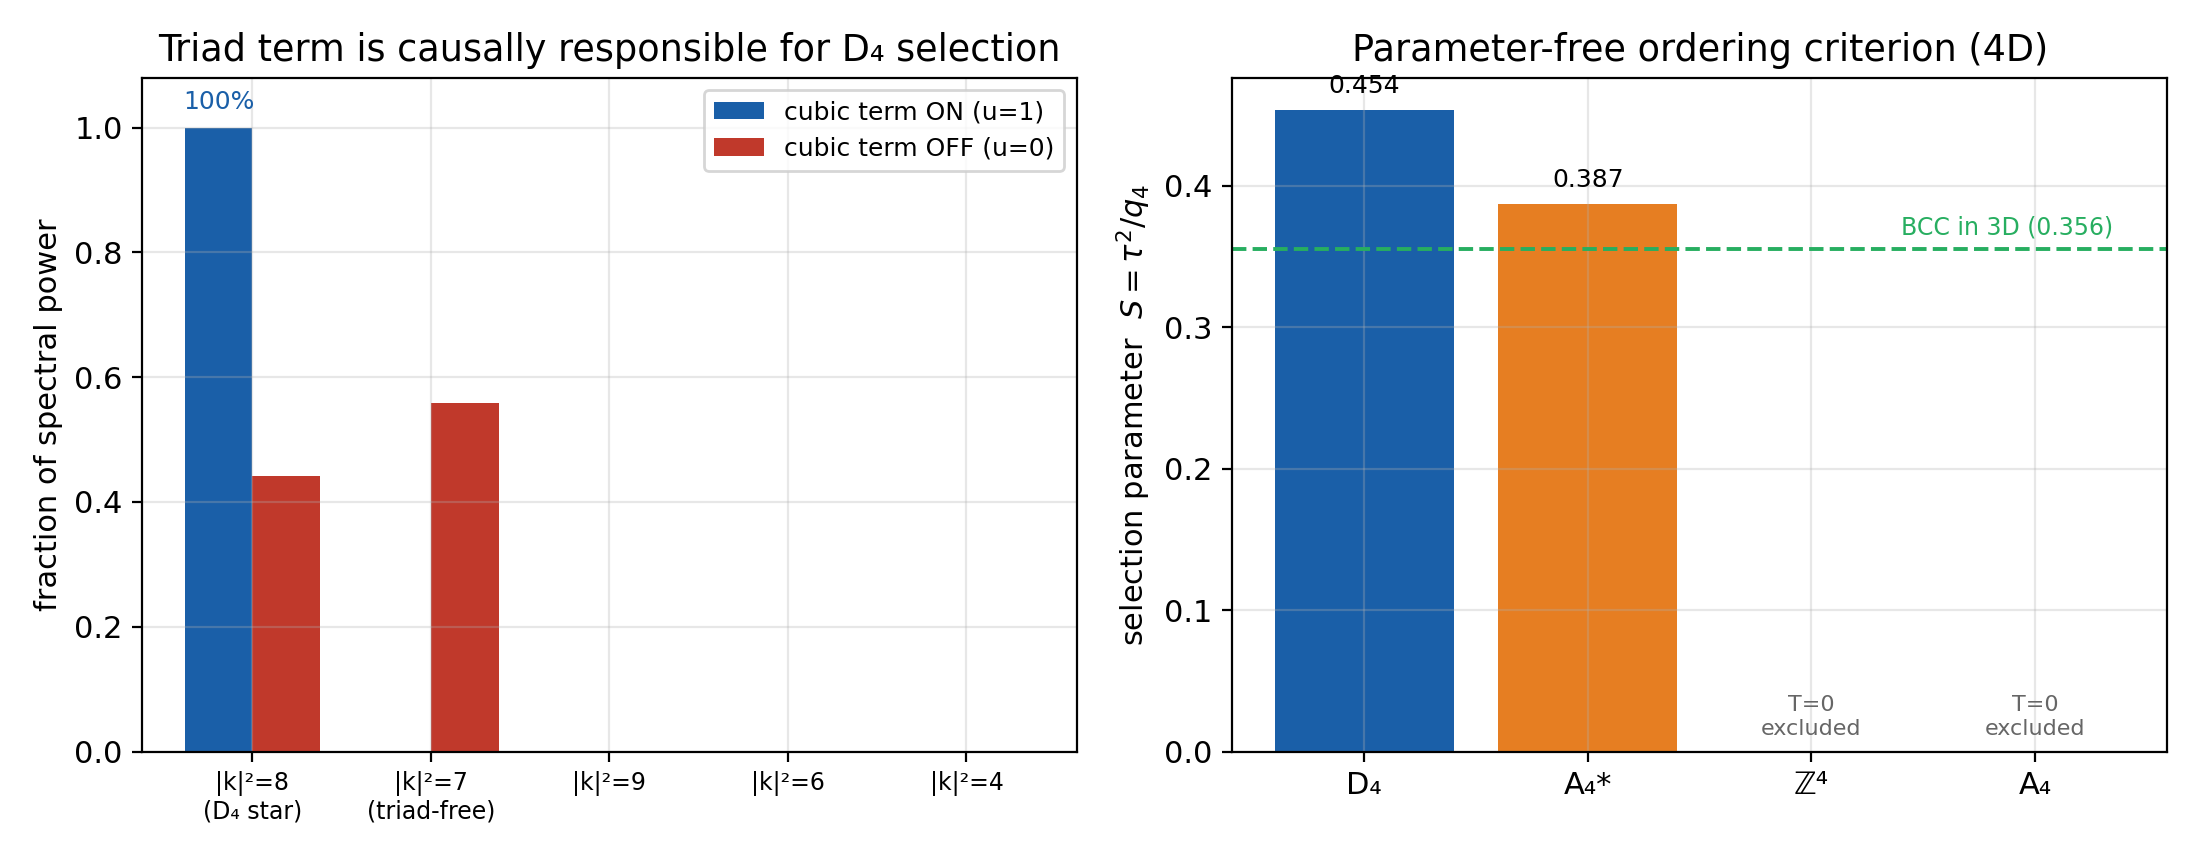
\includegraphics[width=0.85\linewidth]{figs/fig03.png}
\caption{Left: spectral power on the $D_4$ shell with the triad coupling on and off. Right: the criterion $S$ in four dimensions, with the three-dimensional bcc value for scale.}
\label{fig:causal}
\end{figure}

\subsection{Selection from noise}\label{sec:gd3}

The causal test shows what decides a competition between two prescribed shells. It does not show that a featureless field quenched with noise ends in the $D_4$ pattern. That question (gap G-A5) is open, and the evidence on it is of three kinds.

Patterned recovery is established. A field seeded near a $D_4$ pattern recovers it in $12/12$ runs in two cell constructions and in the four-dimensional field, with a parameter sweep on the compute server agreeing ($32/48$ full $D_4$; every pattern family $8/8$) \grade{B, F1--F2}. General selection from broadband noise is not: $0/6$ broadband random starts in the field reached $D_4$ (Wilson $95\%$ upper bound about $39\%$).

The full 24-mode pattern is also rare as an end state of noise quenches at the operating point $(r,\bar\psi)=(-0.35,-0.18)$, where, as Section~\ref{sec:nucleation} shows, the uniform state is metastable. Under the standard quench protocol ($N=16$, $L=\pi$, $q_0^2=8$, $u=v=1$, $\gamma=1$, time step $0.02$, noise $10^{-2}$, $\bar\psi_0=0$), none of $240$ seeds is in the 24-mode pattern at time $t=50$ (Clopper--Pearson two-sided $95\%$ upper bound $1.53\%$), and at $t=500$ none of $60$ seeds at $\gamma=1.0$ and none of $30$ at $\gamma=1.2$ (bounds $[0,0.0596]$ and $[0,0.1157]$) \grade{C, F3/I1}. Most seeds settle in a 6-mode state of excess free energy $-0.04177187933591782$ per unit volume or a 2-mode state at $-0.03653987282038074$; every settled 6-mode state found stays in its family to $t\ge500$ (gaps G-A4 and G-A13).

The third kind of evidence is new. Where the uniform state is linearly unstable, the question changes, because no barrier has to be crossed. Write $r_{\rm eff}=r-2u\bar\psi+3v\bar\psi^2$ for the coefficient that governs the linear growth of shell modes about a uniform field $\bar\psi$ (derived in Section~\ref{sec:band}). At $P_1=(r,\bar\psi)=(-0.35,-0.14)$,
\[
r_{\rm eff}=-0.35+0.28+3(0.0196)=-0.0112<0,
\]
and at $P_2=(-0.5475,-0.2)$, $r_{\rm eff}=-0.5475+0.4+0.12=-0.0275$, the largest $|r_{\rm eff}|$ among the barrier-free points of the band computation. In a box of side $L=3\pi$ ($N=24$, checks at $N=32$) the unstable shell is $|\mathbf{n}|^2=18$, with $312$ modes in three orbits: $24$ of type $(3,3,0,0)$, $96$ of type $(4,1,1,0)$ and $192$ of type $(3,2,2,1)$. Model~B quenches from mean-free white noise of amplitude $10^{-3}$ were run by two code- and binary-independent routes (a numpy semi-implicit scheme and a C/FFTW exponential integrator with its own noise generator). At $P_1$ the end state is a $D_4$ root system in $29$ of $30$ pooled runs (Wilson interval $[0.833,0.994]$) \grade{F2/I1}. These $D_4$ states are mostly rotated: the shell contains $41$ subsystems isometric to the $D_4$ roots, mixing the three orbits, and the states found are degenerate with the axis-aligned $(3,3,0,0)$ star and with the $L=\pi$ value $F_{D_4}=-0.012836702440212955$ to $3\times10^{-16}$. One rotated system, which our own check reproduces, consists of $6$ vectors of type $(3,3,0,0)$, $6$ of type $(4,1,1,0)$ and $12$ of type $(3,2,2,1)$. At $P_2$ the $D_4$ fraction is $41/50=0.82$ (interval $[0.692,0.902]$) \grade{F2/I1}. The remaining runs end in a $42$-mode state of rank $4$ that is not $D_4$, lies $7.714\times10^{-4}$ above it, and is a strict local minimum (Hessian gap $+0.0445$ at $N=32$) \grade{F3/I1}. The control at the metastable point $P_0=(-0.35,-0.18)$ stays uniform in $15/15$ runs. A frozen ten-seed label at $P_2$ came out ``selects'' on one route and ``mixed'' ($7/10$) on the other, so that label is seed-dependent and is not established; the fraction above is the record (gap G-D3).

So within the barrier-free sliver, at $L=3\pi$, noise selects $D_4$ with high probability, and $D_4$ is always the lowest state found. The sharpest open form of G-A5 and G-D3 is whether the basin fraction $p_{D_4}(r,\bar\psi,L)$, about $0.97$ at $P_1$ and $0.82$ at $P_2$ here, tends to $1$, stays below $1$ or falls as the box grows. A box of side $4\pi$ contains only the $(4,4,0,0)$ star, so the next informative box is $L=5\pi$; the noise strength and the prior on $\bar\psi$ for that run are inputs still to be fixed.

%===========================================================================
\section{Baseline tension and the phase band}\label{sec:band}
%===========================================================================

\subsection{An omission, and its repair}

The annealed run of Section~\ref{sec:sim} populated only $6$ of the $24$ modes. This prompted a comparison the analysis of Section~\ref{sec:selection} had not made: not against other lattices, but against sub-patterns of the $D_4$ shell. At zero baseline field a hexagonal sub-pattern of $6$ modes has lower free energy than the full $24$-mode pattern at every quench depth tested. The simulation was right and the analysis incomplete.

The missing variable is the baseline tension $\bar\psi$, the spatial mean of the field. To bring it in we expand the free energy about the mean and subtract the free energy of the uniform state, so that only the terms carried by the pattern remain. Write $\psi=\bar\psi+\varphi$ with $\langle\varphi\rangle=0$. Expanding the powers and averaging,
\begin{align*}
\langle\psi^2\rangle&=\bar\psi^2+\langle\varphi^2\rangle,\\
\langle\psi^3\rangle&=\bar\psi^3+3\bar\psi\langle\varphi^2\rangle+\langle\varphi^3\rangle,\\
\langle\psi^4\rangle&=\bar\psi^4+6\bar\psi^2\langle\varphi^2\rangle+4\bar\psi\langle\varphi^3\rangle+\langle\varphi^4\rangle ,
\end{align*}
the terms linear in $\varphi$ vanishing on average. Insert these in the free energy \eqref{eq:F}, with the shell modes annihilated by the gradient operator, and subtract the free energy of the uniform state, which removes every term without $\varphi$. Collecting the rest by the power of $\varphi$, the coefficient of $\langle\varphi^2\rangle$ is $\tfrac r2-\tfrac u3\cdot3\bar\psi+\tfrac v4\cdot6\bar\psi^2$, that of $\langle\varphi^3\rangle$ is $-\tfrac u3+\tfrac v4\cdot4\bar\psi$, and that of $\langle\varphi^4\rangle$ is $\tfrac v4$. Hence
\begin{equation}\label{eq:Fexcphi}
\frac{F_{\rm exc}}{V}=\tfrac12\big(r-2u\bar\psi+3v\bar\psi^2\big)\langle\varphi^2\rangle-\tfrac13\big(u-3v\bar\psi\big)\langle\varphi^3\rangle+\tfrac v4\langle\varphi^4\rangle .
\end{equation}
For the equal-amplitude shell state of Section~\ref{sec:selection}, $\langle\varphi^2\rangle=NA^2$, $\langle\varphi^3\rangle=TA^3$ and $\langle\varphi^4\rangle=QA^4$, so
\begin{equation}\label{eq:Fmod}
\frac{F_{\rm exc}}{V}=\frac N2\,r_{\rm eff}\,A^2-\frac T3\,u_{\rm eff}\,A^3+\frac{vQ}{4}A^4,\qquad
r_{\rm eff}=r-2u\bar\psi+3v\bar\psi^2,\quad u_{\rm eff}=u-3v\bar\psi .
\end{equation}
\lbl{Derivation} The baseline tension tunes the triad coupling, $u_{\rm eff}=u-3v\bar\psi$. It is not a nuisance parameter. It is the control parameter of the selection mechanism, and it is the quantity the ontology names as primitive.

\subsection{The band}

\lbl{Prediction} Figure~\ref{fig:phase} shows the result of minimising over a frozen set of competitors in the window $\bar\psi\in[-0.6,0.2]$, $r\in[-0.6,0.1]$. The full $24$-mode pattern is the ground state on a contiguous band along the boundary with the disordered phase, spanning roughly $-0.33\lesssim\bar\psi\lesssim0.05$. Lower-symmetry sub-patterns occupy the region of higher tension.

The canonical value of the band fraction is
\begin{equation}\label{eq:band}
\frac{758}{6561}=11.5531\%,
\end{equation}
under the following definition, which we state in full because the number depends on it. The window is sampled on an $81\times81$ grid (hence $6561$ points). At each point the free energy of the full field is relaxed at fixed $\bar\psi$ in a periodic box of side $L=\pi$, one period of the pattern per direction, on a $16^4$ grid, with $q_0^2=8$, $u=v=1$, shell detuning zero and no sextic term ($w_6=0$). The competitors are a frozen set of seeded sub-patterns of the shell, stripes, a decorated stripe and 20-mode proxies. The point counts for $D_4$ if the relaxed $24$-mode state has the lowest free energy \grade{F3/I1}. Two related numbers clarify what the band depends on. Restricting the competitors to the hexagonal 6-mode pattern alone gives $12.9706\%$; and the one-mode approximation on the same grid gives $756/6561=11.5226\%$. On a finer $161\times161$ grid the one-mode value is $11.60\%$, and with conserved-$\bar\psi$ common tangents it is $11.42\%$. A value of $11.85\%$ appeared in an earlier record and $11.90\%$ in a cross-check; neither can be reproduced from any recorded definition, and neither should be cited.

\begin{figure}[htbp]
\centering
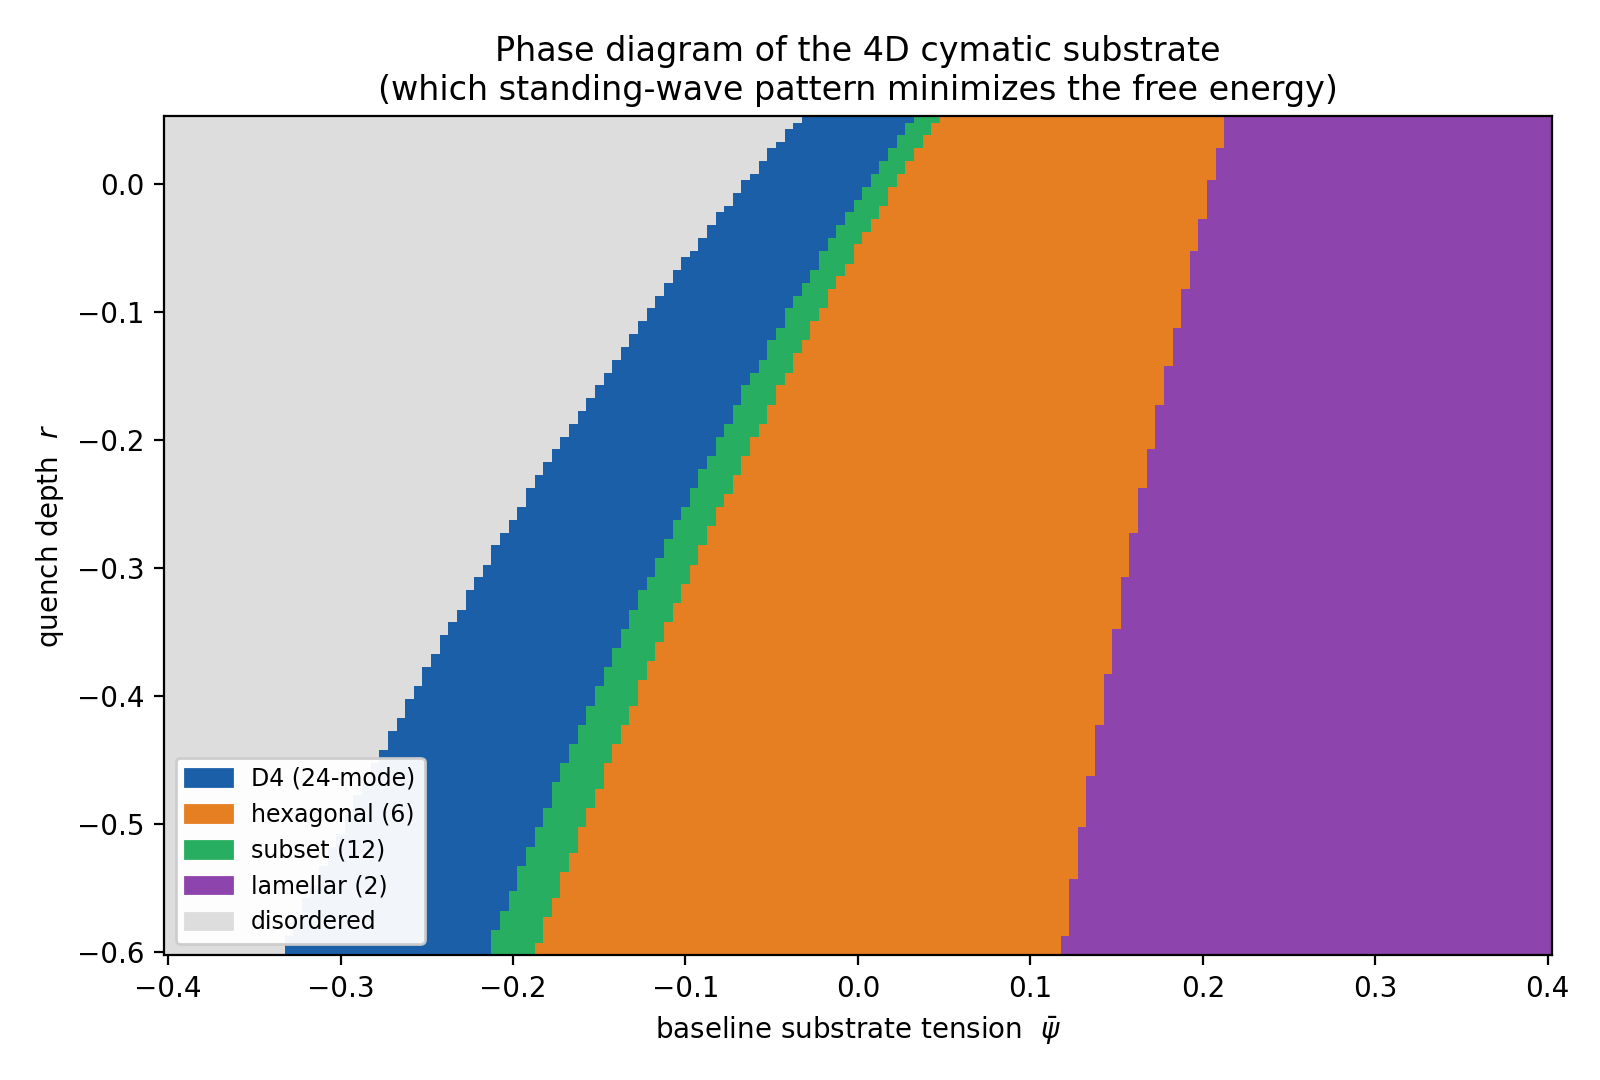
\includegraphics[width=0.8\linewidth]{figs/fig04.png}
\caption{Phase diagram in the plane of baseline tension $\bar\psi$ and quench depth $r$. The full 24-mode $D_4$ state occupies a contiguous band along the boundary with the disordered phase.}
\label{fig:phase}
\end{figure}

The band lies along the order--disorder boundary, which is where the ``orders first'' argument of Section~\ref{sec:selection} says it should be. Two calculations made for different reasons agree on where the $D_4$ phase is.

\subsection{Detuning}

The band was computed with the shell exactly on resonance. A real shell at $|\mathbf{k}|^2=8$ pays the penalty $(q_0^2-8)^2$, so the effective quench depth on the shell is $r_{\rm shell}=r+(q_0^2-8)^2$. At $r=-0.35$ and $\bar\psi=-0.18$: for $q_0^2=8$ the penalty is zero and the ordered branch exists, with $A^*=0.0776$ and $F_{\rm exc}/V=-0.00763$; for $q_0^2=7.5$ the penalty is $0.25$, $r_{\rm shell}=-0.10$, and the ordered branch has disappeared. A detuning of $0.5$ in $q_0^2$ removes the $D_4$ phase.

\lbl{Input} The $D_4$ band is conditional on $q_0$ being tuned onto the shell. Since $a_0=2\pi/q_0$, this says that the resonant wavelength of the substrate must match the lattice it forms. That is self-consistent, but it is a condition, and it must accompany every citation of the band value \eqref{eq:band}.

Sixth-order terms narrow the band without removing it. For the $D_4$ shell the number of ordered closed $6$-tuples of shell vectors is $H=911{,}040$ (computed by FFT convolution, validated against direct enumeration at third and fourth order, and reproduced by the Lean kernel under this reading of $H$, claim C17). Adding a sextic term $\tfrac{w_6}{6}HA^6$ to the one-mode free energy reduces the one-mode band from $11.60\%$ at $w_6=0$ to $8.36\%$ at $w_6=0.2$.

%===========================================================================
\section{The ordered state}\label{sec:stability}
%===========================================================================

\subsection{The one-mode state and the relaxed field}

Take $N=24$, $T=192$, $Q=3384$, $r=-0.35$, $\bar\psi=-0.18$, $u=v=1$ and $q_0^2=8$. Then $r_{\rm eff}=0.1072$ (the arithmetic is displayed in Section~\ref{sec:nucleation}) and $u_{\rm eff}=u-3v\bar\psi=1.54$, and the stationarity condition of the excess free energy \eqref{eq:Fmod} has a real ordered root at per-mode amplitude $A^*=0.0775753$ with $F_{\rm exc}/V=-0.0076323$.

Here $F_{\rm exc}$ is the excess over the uniform state, so the disordered phase has $F_{\rm exc}=0$. The absolute density differs by the uniform value
\[
\tfrac12(r+q_0^4)\bar\psi^2-\tfrac u3\bar\psi^3+\tfrac v4\bar\psi^4=1.0333364,
\]
in which the $k=0$ term $\tfrac12q_0^4\bar\psi^2$ is not an irrelevant constant: under conserved dynamics it sets the convexity of the uniform branch, and the coexistence-aware band of Section~\ref{sec:band} depends on it.

The one-mode state is a variational trial state, so its free energy bounds the true minimum from above. Relaxing it under Model~B lets the field develop the harmonics the ansatz excludes, and gives $F_{\rm exc}/V=-0.0077276$. An independent review had found $-0.007728$ and attributed the difference from $-0.0076323$ to the uniform baseline. That attribution cannot be right, since the difference is $9.53\times10^{-5}$ and the baseline is $1.03$. The difference is harmonic lowering, and it measures the accuracy of the one-mode approximation: $9.53\times10^{-5}/0.0076323=1.25\%$ of the one-mode value.

\subsection{Dynamical stability}

Seed the full pattern at $A^*=0.0776$ with all $24$ modes in phase, and evolve.

\begin{table}[htbp]
\centering
\begin{tabular}{lrrrr}
\toprule
dynamics & final $\bar\psi$ & $D_4$ shell power & modes & rms modulation\\
\midrule
seed & $-0.18000$ & $1.0000$ & $24/24$ & $0.3802$\\
Model~B (conserved) & $-0.18000$ & $1.0000$ & $24/24$ & $0.3806$\\
Model~A (non-conserved) & $+0.00087$ & $1.0000$ & $24/24$ & $0.4206$\\
\bottomrule
\end{tabular}
\caption{Seeded evolution of the symmetric 24-mode state.}
\label{tab:attractor}
\end{table}

Under Model~B the baseline is held exactly, all $24$ modes stay occupied and the amplitude is unchanged to four figures: the symmetric $D_4$ standing wave is a dynamical attractor, not only a minimum of $F$. Over a long horizon the rms modulation stays at $0.380565$ and $\max|\psi|$ at $1.689598$, constant to six figures from $t=2$ to $t=18$. Under Model~A the pattern stays symmetric while $\bar\psi$ drifts to $+0.00087$, outside the band. That persistence is not metastability. At $(r,\bar\psi)=(-0.35,+0.00087)$ on the $16^4$ grid with $L=\pi$, the drifted state is a saddle of $F$: apart from the four translation zero modes its Hessian has a $9$-fold degenerate negative eigenvalue $\lambda\approx-0.0646$, carrying one irreducible representation of $W(F_4)$, the point group of the $D_4$ lattice (Section~\ref{sec:algebra}) \grade{index F2/I1; instability F3/I1}. The seeded run stays on the saddle only because an exactly symmetric seed lies in an invariant subspace; a random perturbation of size $10^{-4}$ sends noise-free Model~A to a lower 6-mode state in $9$ of $9$ trials.

Linear stability of the Model~B state has been sampled three ways that agree: $52$ sector fibres, $259$ wavevectors on one machine and $14{,}641$ on a dense map. On the dense map exactly one wavevector has a positive rate, the Goldstone mode at $\mathbf{q}=0$, at round-off level $8.67\times10^{-12}$, and the least-damped nonzero rate is $-2.13324\times10^{-5}$ \grade{C}. The $52$ values are maxima over sectors, not over full fibres, and the first finite rate at the zone centre differs by $3.05\times10^{-4}$ between two routes, a difference attributed to sector coverage but not proved.

A direct test of the relaxed state was added in this edition. Doubling the box to $L=2\pi$ ($N=16$) admits perturbations with wavevectors outside $2\mathbb{Z}^4$, the subharmonic or ``odd'' sector, which a box of side $\pi$ cannot represent. At three points $(r,\bar\psi)=(-0.35,-0.18)$, $(-0.35,-0.22)$ and $(-0.35,-0.15)$ the odd-sector Hessian has no negative eigenvalue; its smallest eigenvalues are $1.0417619866$, $1.0711951433$ and $1.0204460536$. The smallest nonzero eigenvalue over all sectors is $0.3423000506$, $0.4305432217$ and $0.2718504312$ respectively, in a cluster of $9$ that splits $6+3$ \grade{F2/I1}. This is a finite-box statement at three points; it does not establish continuum stability for all $\mathbf{q}$, and an earlier claim from an outside model of three subharmonic negative modes at these points is refuted. The sharpest remaining problem for the stability question is a certified, interval-enclosed bound on the Bloch spectrum over the whole Brillouin zone.

Every earlier simulation started from noise reached only a $6$- or $12$-mode sub-pattern at the operating point; the seeded runs above were the first confirmation of the full symmetric state, and the barrier-free quenches of Section~\ref{sec:gd3} the first from noise.

%===========================================================================
\section{The transition and nucleation}\label{sec:nucleation}
%===========================================================================

\subsection{The transition is first order}

At $\bar\psi=-0.18$, with $r=-0.35$ and $u=v=1$,
\begin{equation}\label{eq:reffop}
r_{\rm eff}=r-2u\bar\psi+3v\bar\psi^2=-0.35+0.36+0.0972=+0.1072>0 .
\end{equation}
The uniform state is linearly stable, and the $D_4$ state, which has lower free energy, can only be reached by crossing a barrier. At $\bar\psi=-0.10$ the same formula gives $-0.35+0.20+0.03=-0.12$, and at $\bar\psi=0$ it gives $-0.35$; in both cases the uniform state is linearly unstable and pattern grows from noise.

\lbl{Derivation} The transition into the $D_4$ phase at the operating point is first order. Any cosmological use of the framework must supply a nucleation event: a seed, a fluctuation above critical size, or a path through the linearly unstable region at smaller $|\bar\psi|$. Spontaneous emergence from a featureless substrate at this baseline tension does not occur. This was found by misreading a null simulation and then diagnosing it correctly.

\subsection{The critical droplet}

The height of the barrier is the excess free energy of the critical droplet, the saddle point of $F$ that separates the uniform state from the crystal. Version 94 quoted $550.93057$ for this quantity, from a radially restricted amplitude-envelope model, together with an ordinary-differential-equation value of $555$. The thirteenth verification run of the programme (run 13) computed the critical droplet of the unrestricted field (gap G-A10).

At $r=-0.35$, $\bar\psi=-0.18$, $q_0^2=8$, $u=v=1$, under conserved dynamics on periodic boxes of side $12\pi$ to $32\pi$, two code- and binary-independent solvers (numpy and C/FFTW) find a stationary point with residual below $4\times10^{-11}$ and Hessian index $1$ (certified at $12\pi$ and $16\pi$). Its excess free energy extrapolates to
\begin{equation}\label{eq:barrier}
\Delta F^*_\infty=119.06\pm0.03,
\end{equation}
with equivalent radius $R_{\rm eq,\infty}\approx10.465$ \grade{F2/I1}. This is $550.93/119.06\approx4.63$ times lower than the envelope saddle and $555/119.06\approx4.66$ times lower than the ODE value. The envelope state embedded in the full functional is not stationary: its relative gradient is $0.234$, and under the full gradient flow it runs away. So $550.93$ and $555$ are saddles of the restricted model only, and $555$ keeps its grade B within the amplitude equation and nowhere else. The earlier expectation that the full-field value would refine the envelope value by one to ten per cent is refuted.

This changes the reading of the noise-nucleation null of version 94. That null was a negative result in the envelope model: no transition-gate crossings in the $128$ tabulated runs of a $192$-run design ($0/32$ per configuration, a per-configuration $95\%$ gate-entry bound of $8.94\%$, which is not a selection rate), and none in a bounded adaptive multilevel-splitting search ($0/160$, maximum score $0.49474158627843945$) \grade{saddle and thresholds B/F2 within the radial restricted envelope; ensemble null C}. At the noise strength used there, the envelope barrier corresponds to a barrier-to-noise ratio of about $34$, for which a null is expected. The full-field barrier \eqref{eq:barrier} gives about $7.3$ at the same noise, with an uncontrolled prefactor, so the envelope null does not transfer to the full field.

Interface tensions at coexistence were measured on two routes as $0.0189904$ and $0.0264060$, with thin-wall barrier estimates $36.95$ and $138.12$ \grade{B, F1}. Against the envelope saddle these differ by a factor of about $15$; against the full-field droplet the factors are $119.06/36.95\approx3.2$ and $119.06/138.12\approx0.86$. This is an observation, not a claim of agreement: the transferred tension is path-dependent by $40\%$. The amplitude-equation barrier is about $15$ times the thin-wall value; the full-field barrier is within a factor of about $3.2$.

\subsection{The rate}

The rate is open. In finite boxes the unstable eigenvalue $\lambda_-$, the prefactor quantities $\kappa$ and $J$ and the count $n_0=4$ of zero modes are determined \grade{F2/I1}. The one-loop logarithmic determinant, which a Langer rate needs, diverges logarithmically in the ultraviolet in four dimensions \grade{mechanism F2/I1}. With a tadpole subtraction the renormalised value is about $-41\,\Delta F$ \grade{F3/I1, one route}, which makes the Gaussian approximation uncontrolled for any noise strength at which an event would occur; that noise strength is about $\varepsilon^*\approx0.046$--$0.048$, conditional on the subtraction \grade{F3/I1}. The value $n_0=10$ in infinite volume is claimed but not checked. The sharpest remaining problem is the rate at a stated noise strength under a stated ultraviolet prescription, computed beyond Gaussian order, for instance by forward-flux sampling of Model~B started from the certified saddle. The noise strength and the prescription are modelling choices still to be made.

%===========================================================================
\section{Elastic constants and phonons of the $D_4$ crystal}\label{sec:phonons}
%===========================================================================

The ordered state is a crystal, and a crystal has phonons. Their speeds are the first place where the pattern of Sections~\ref{sec:selection}--\ref{sec:stability} meets a physical question about spacetime, because any reading of the pattern as a medium in which signals propagate must say how fast they go. This section computes the long-wavelength spectrum in the manner of continuum elasticity theory~\cite{ref47}: first the elastic constants of the one-mode state in closed form, then the relaxed numerical values, then what follows.

\subsection{Elastic constants of the one-mode state}

Let the crystal be displaced by a slowly varying field $\mathbf{u}(\mathbf{x})$, so that $\psi(\mathbf{x})\to\psi(\mathbf{x}-\mathbf{u}(\mathbf{x}))$. For a uniform strain $\varepsilon_{ij}=\partial_ju_i$, the plane wave $e^{i\mathbf{G}\cdot\mathbf{x}}$ becomes $e^{i\mathbf{G}\cdot(\mathbf{x}-\varepsilon\mathbf{x})}=e^{i\mathbf{G}'\cdot\mathbf{x}}$ with $\mathbf{G}'=\mathbf{G}-\varepsilon^{\mathsf T}\mathbf{G}$, and
\[
|\mathbf{G}'|^2=|\mathbf{G}|^2-2\,G_i\varepsilon_{ij}G_j+O(\varepsilon^2).
\]
A uniform strain is a linear map of wavevectors, so closed triads and quadruples stay closed and $\langle\varphi^2\rangle$, $\langle\varphi^3\rangle$, $\langle\varphi^4\rangle$ do not change. The only change is in the gradient term, where each mode now pays $(q_0^2-|\mathbf{G}'|^2)^2$. Since $|\mathbf{G}|^2=q_0^2$ on the shell, the term of order $\varepsilon^2$ in $|\mathbf{G}'|^2$ is multiplied by $q_0^2-|\mathbf{G}|^2=0$, and to second order
\[
(q_0^2-|\mathbf{G}'|^2)^2=4\,(G_i\varepsilon_{ij}G_j)^2 .
\]
With $\varphi=A\sum_{\mathbf{G}}e^{i\mathbf{G}\cdot\mathbf{x}}$ and $\langle\tfrac12\varphi(q_0^2+\nabla^2)^2\varphi\rangle=\tfrac12A^2\sum_{\mathbf{G}}(q_0^2-|\mathbf{G}'|^2)^2$, the elastic energy density is
\begin{equation}\label{eq:fel}
f_{\rm el}=2A^2\sum_{\mathbf{G}}G_iG_jG_kG_l\,\varepsilon_{ij}\varepsilon_{kl}\equiv\tfrac12\,C_{ijkl}\,\varepsilon_{ij}\varepsilon_{kl},\qquad C_{ijkl}=4A^2\sum_{\mathbf{G}}G_iG_jG_kG_l .
\end{equation}
Now use the design property. On the shell of Section~\ref{sec:sim} the $24$ vectors are $\mathbf{G}=2\alpha$, $\alpha\in\Phi$, with $|\mathbf{G}|^2=8$. Because they form a 5-design, the fourth-moment tensor is isotropic, $\sum_{\mathbf{G}}G_iG_jG_kG_l=c\,(\delta_{ij}\delta_{kl}+\delta_{ik}\delta_{jl}+\delta_{il}\delta_{jk})$. Contracting $i=j$ and $k=l$ gives $\sum_{\mathbf{G}}|\mathbf{G}|^4=24\cdot64=1536$ on the left and $c\,(16+4+4)=24c$ on the right, so $c=64$ and
\begin{equation}\label{eq:Cijkl}
C_{ijkl}=256A^2\,(\delta_{ij}\delta_{kl}+\delta_{ik}\delta_{jl}+\delta_{il}\delta_{jk}),\qquad C_{1111}=768A^2,\quad C_{1122}=C_{1212}=256A^2 .
\end{equation}
Comparing with the isotropic form $C_{ijkl}=\lambda\delta_{ij}\delta_{kl}+\mu(\delta_{ik}\delta_{jl}+\delta_{il}\delta_{jk})$ identifies the Lamé constants,
\begin{equation}\label{eq:lame}
\lambda=\mu=256A^2 .
\end{equation}
The equality $\lambda=\mu$ is a Cauchy relation, $C_{1122}=C_{1212}$, here forced by the geometry of the shell rather than by central forces. At the one-mode amplitude $A=0.0775753$ of Section~\ref{sec:stability}, $256A^2=1.5405892$, which agrees with the stiffness $\lambda=\mu=1.54058921014457$ quoted in version 94. The agreement suggests that the version~94 number is the one-mode stiffness of the one-mode state rather than a property of the relaxed crystal; the script that produced it has not been traced, so this reading is a candidate.

The inertia comes from the term $\partial_t^2\psi$ of the damped wave equation \eqref{eq:dw}, whose kinetic density is $\tfrac12(\partial_t\psi)^2$. For a time-dependent displacement, $\partial_t\psi=-\nabla\psi\cdot\dot{\mathbf{u}}$, and averaging over a cell,
\[
\langle(\partial_t\psi)^2\rangle=A^2\sum_{\mathbf{G}}(\mathbf{G}\cdot\dot{\mathbf{u}})^2=A^2\,\dot u_i\dot u_j\sum_{\mathbf{G}}G_iG_j=A^2\cdot\frac{24\cdot8}{4}\,|\dot{\mathbf{u}}|^2=48A^2|\dot{\mathbf{u}}|^2,
\]
using the isotropy of the second moment. So the mass density of the crystal is $\rho=48A^2$.

\subsection{Sound speeds}

The equation of motion for $\mathbf{u}$ is $\rho\,\ddot u_i=C_{ijkl}\,\partial_j\partial_lu_k$. For a plane wave $\mathbf{u}=\mathbf{e}\,e^{i(\mathbf{q}\cdot\mathbf{x}-\omega t)}$ with the isotropic Lamé form \eqref{eq:lame} this reads
\begin{equation}\label{eq:phononeom}
\rho\,\omega^2\,\mathbf{e}=(\lambda+\mu)\,\mathbf{q}\,(\mathbf{q}\cdot\mathbf{e})+\mu\,|\mathbf{q}|^2\,\mathbf{e}.
\end{equation}
Taking the polarisation along and across $\mathbf{q}$ separates \eqref{eq:phononeom} into its two eigenspaces. A longitudinal wave, $\mathbf{e}\parallel\mathbf{q}$, has $\rho\omega^2=(\lambda+2\mu)|\mathbf{q}|^2$; each of the three transverse waves, $\mathbf{e}\perp\mathbf{q}$, has $\rho\omega^2=\mu|\mathbf{q}|^2$. Hence
\begin{equation}\label{eq:speeds}
c_L^2=\frac{\lambda+2\mu}{\rho}=\frac{768}{48}=16,\qquad c_T^2=\frac{\mu}{\rho}=\frac{256}{48}=\frac{16}{3},\qquad \frac{c_L^2}{c_T^2}=3 .
\end{equation}
\lbl{Derivation} At one-mode order the $D_4$ crystal has four gapless acoustic branches, one longitudinal and three transverse, with exactly isotropic dispersion at order $q^2$ and $c_L/c_T=\sqrt3$ \grade{B, [MV]4D/I1; SymPy and Wolfram}. The ratio does not depend on $A$, $r$ or $\bar\psi$. The same steps apply to any scalar density wave on a single shell that is a spherical 4-design, in any dimension $d$, and always give $c_L^2/c_T^2=3$ at this order: the Cauchy relation follows from the isotropy of the fourth moment alone \grade{B, [MV]4D/I1}.

The relaxed crystal, with harmonics, was computed by two routes (Python with OpenBLAS, and Wolfram Engine~15.0) at $L=\pi$, $(r,\bar\psi)=(-0.35,-0.18)$, $u=v=1$, $q_0^2=8$, $w_6=0$ and damping taken to zero. Its excess free energy is $-0.0077276236034$. The spectrum has four gapless branches, three transverse and one longitudinal, with linear dispersion, and an optical gap of $0.342300$; the values are
\[
c_T^2=5.332526\ (\text{three branches}),\qquad c_L^2=15.996363,\qquad \frac{c_L}{c_T}=1.731985,
\]
the two routes agreeing to $2\times10^{-8}$ \grade{F2/I1}. The relaxed stiffness is $\mu_{\rm relaxed}=c_T^2\rho=1.54465$ with $\rho=0.2896648$ \grade{F2/I1}, and $\lambda_{\rm relaxed}=1.54447$ \grade{F3/I1}; the relaxed amplitude is $A=0.0776817$, at which $256A^2=1.54482$. The relaxed values sit about $0.26\%$ above the one-mode stiffness of version 94, as one expects from a different state, and the Cauchy relation survives relaxation to within $0.012\%$. Version 94 reported a long-wavelength ratio ``$L/T=3.016$ against $3$''; that is $c_L^2/c_T^2$ at $|\mathbf{q}|=0.02$ along $e_1$, including the $q^2$ correction (the transverse branch is lower by $0.54\%$ there), and its limit as $\mathbf{q}\to0$ is $2.99977$ \grade{F2/I1}. The record number is explained, not wrong.

The first directional dependence of the phonon spectrum appears at order $q^4$ in $\omega^2$, through the degree-6 harmonic invariant $P_6$ of $W(F_4)$; counting invariants of $W(F_4)$ shows that the $q^2$ tensor must be isotropic \grade{B; GAP and SymPy}. The coefficients of $P_6$, in the normalisation of the run record, are $\xi_{6,L}=-81.78\pm0.02$ and $\xi_{6,T}=27.260\pm0.008$. The cubic coupling between one longitudinal and two transverse phonons is nonzero and negative; its numerical value is not settled.

\subsection{A single sound speed is impossible in a stable isotropic solid}

The ratio $c_L/c_T=\sqrt3$ is not a feature of this model alone. For an isotropic solid in $d$ dimensions with bulk modulus $K=\lambda+2\mu/d$, we express the speed ratio through $K$ and then ask what a common speed would require. Substituting $\lambda=K-2\mu/d$,
\[
\frac{c_L^2}{c_T^2}=\frac{\lambda+2\mu}{\mu}=\frac{K-2\mu/d+2\mu}{\mu}=\frac K\mu+2-\frac2d,
\]
which in four dimensions is $K/\mu+3/2$. A common speed, $c_L=c_T$, would need $K/\mu=-1/2$, that is $K=-\mu/2<0$. But the elastic energy of an isotropic solid, $\mu\,\tilde\varepsilon_{ij}\tilde\varepsilon_{ij}+\tfrac K2(\varepsilon_{kk})^2$ with $\tilde\varepsilon$ the traceless part of the strain, is positive definite only if $\mu>0$ and $K>0$. So no stable isotropic four-dimensional solid has a single sound speed \grade{B}. The Cauchy relation $\lambda=\mu$ gives $K=3\mu/2$ and the ratio $3$ of the sound speeds \eqref{eq:speeds}.

\subsection{Damping and compactification}

At the damping $\gamma=1.2$ used in the quenches of Section~\ref{sec:sim}, the phonons are not waves at long wavelength. Adding the damping of the wave equation \eqref{eq:dw} to the equation of motion gives $\omega^2+i\gamma\omega=c^2q^2$, with roots $\omega=-\tfrac{i\gamma}2\pm\sqrt{c^2q^2-\gamma^2/4}$. They are overdamped when $cq<\gamma/2$, that is for $q<0.6/4=0.15$ on the longitudinal branch and $q<0.6\sqrt3/4\approx0.26$ on the transverse ones. Below those wavenumbers the long-wave dynamics is diffusive, with dynamic exponent $z=2$, not propagating with $z=1$ \grade{F2/I1}. Version 94 made no claim that these modes propagate, so nothing in it is contradicted.

Suppose one direction of the base is compactified, as one reading of Section~\ref{sec:dimension} requires. Take the circle along $e_4$ with circumference $n\pi$, or along the root direction $(1,1,0,0)/\sqrt2$ with circumference $n\pi\sqrt2$, for $n=1,\dots,4$, so that the crystal fits. At zero momentum along the circle the four acoustic branches remain gapless and keep two speeds: for $\mathbf{q}$ in the three open directions there is one longitudinal branch at $c_L$, and three transverse branches at $c_T$, one of them polarised along the circle \grade{F2/I1}. The tower of Kaluza--Klein gaps is listed in Table~\ref{tab:kk}; these numbers describe the model in those boxes and are not predictions.

\begin{table}[htbp]
\centering
\begin{tabular}{lrrrr}
\toprule
circle & $n=1$ & $n=2$ & $n=3$ & $n=4$\\
\midrule
$e_4$, circumference $n\pi$ & $15.885129$ & $1.249101$ & $0.437521$ & $0.289598$\\
root, circumference $n\pi\sqrt2$ & $3.991685$ & $0.591699$ & $0.391461$ & $0.357808$\\
\bottomrule
\end{tabular}
\caption{Lowest Kaluza--Klein gaps of the relaxed $D_4$ crystal compactified on a lattice circle \grade{F2/I1; root circle at $n=2,3,4$ F3/I1}.}
\label{tab:kk}
\end{table}

The modified phase-field-crystal dynamics mentioned in Section~\ref{sec:substrate} adds a conserved density mode; a single verifier-side computation found five gapless branches with three speeds \grade{F3/I1}. It does not restore a single speed.

%===========================================================================
\section{The site-field formulation, retained with its scope}\label{sec:legacy}
%===========================================================================

Version 92 described the substrate by a field $\phi(n,s)$ living on the sites $n$ of a $D_4$ lattice of spacing $a_0$ and on integer time steps $s$ of length $\Delta t$. Section~\ref{sec:substrate} retired that formulation as a description of the substrate. Its mathematics is still correct, and three of its results (an exact dispersion relation, a stability bound for any discrete implementation, and a corrected non-relativistic limit) are needed later. We keep them here, for that formulation only.

\subsection{Action, equation of motion and dispersion}

The action is
\begin{equation}\label{eq:siteaction}
S=\sum_{n,s}a_0^4\Delta t\left[\frac{M^*}{2}\Big(\frac{\phi(n,s{+}1)-\phi(n,s)}{\Delta t}\Big)^2-\frac{J}{2a_0^2}\sum_{\alpha\in\Phi}\big(\phi(n{+}\alpha,s)-\phi(n,s)\big)^2-\frac{\mu^2}{2}\phi(n,s)^2\right],
\end{equation}
with inertia $M^*>0$, coupling $J>0$ and mass parameter $\mu^2\ge0$; here $n+\alpha$ denotes the neighbouring site displaced by $a_0\alpha$. Varying $\phi(n,s)$ and collecting the contributions of the two time links and the $24$ spatial links that contain it (each neighbour bond appears twice in the double sum, once from each end) gives
\begin{equation}\label{eq:eom}
M^*\big[\phi(n,s{+}1)-2\phi(n,s)+\phi(n,s{-}1)\big]=\frac{2J\Delta t^2}{a_0^2}\sum_{\alpha}\big[\phi(n{+}\alpha,s)-\phi(n,s)\big]-\Delta t^2\mu^2\phi(n,s).
\end{equation}
Substitute $\phi=e^{i(a_0\mathbf{k}\cdot n-\omega s\Delta t)}$. The left side becomes
\[
M^*(e^{-i\omega\Delta t}-2+e^{i\omega\Delta t})\,\phi=-4M^*\sin^2(\omega\Delta t/2)\,\phi,
\]
and the sum becomes $\sum_\alpha(e^{ia_0\mathbf{k}\cdot\alpha}-1)\phi=-\sum_\alpha(1-\cos a_0\mathbf{k}\cdot\alpha)\phi$, the sine parts cancelling between $\alpha$ and $-\alpha$. Dividing by $-4M^*\phi$,
\begin{equation}\label{eq:disp}
\sin^2\!\Big(\frac{\omega\Delta t}{2}\Big)=\frac{\Delta t^2}{4M^*}\Big[\frac{2J}{a_0^2}\sum_{\alpha\in\Phi}\big(1-\cos(a_0\mathbf{k}\cdot\alpha)\big)+\mu^2\Big].
\end{equation}
The lattice sum has a closed form. For a fixed pair $\{i,j\}$, apply $\cos(X+Y)+\cos(X-Y)=2\cos X\cos Y$ with $X=a_0k_i$, $Y=a_0k_j$ to the sign pairs $(+,+),(+,-)$ and again to $(-,-),(-,+)$; the four roots give $4\cos(a_0k_i)\cos(a_0k_j)$. Summing over the six pairs,
\begin{equation}\label{eq:cosid}
\sum_{\alpha\in\Phi}\cos(a_0\mathbf{k}\cdot\alpha)=4\sum_{i<j}c_ic_j=2\Big[\Big(\sum_ic_i\Big)^2-\sum_ic_i^2\Big],\qquad c_i=\cos(a_0k_i).
\end{equation}
Expanding \eqref{eq:disp} for small $\mathbf{k}$ with $1-\cos x=x^2/2-x^4/24+\dots$ reproduces the moment identities \eqref{eq:moments} term by term, by a route (Euler--Lagrange variation followed by a root sum) independent of the direct computation of Section~\ref{sec:geometry}.

The energy conjugate to \eqref{eq:eom} is a sum of three terms, a kinetic square with coefficient $M^*/2$, a gradient square with coefficient $J/(2a_0^2)$ and a mass term $\mu^2\phi^2/2$. For $M^*,J>0$ and $\mu^2\ge0$ each is non-negative, so the discrete Hamiltonian is bounded below and the vacuum $\phi=0$ is stable. This statement concerns the second-order-in-time site field. It is not a statement about the Euclidean measure of Section~\ref{sec:rp}, and the two do not conflict.

\subsection{The stability bound}

Real frequencies require $\sin^2(\omega\Delta t/2)\le1$ for every $\mathbf{k}$. We first find the largest value of the lattice sum over the Brillouin zone, then express the prefactor of \eqref{eq:disp} through a wave speed. That lattice sum is the bracket $\sum_\alpha(1-\cos a_0\mathbf{k}\cdot\alpha)=24-\sum_\alpha\cos(a_0\mathbf{k}\cdot\alpha)$. By the cosine identity \eqref{eq:cosid}, $\sum_\alpha\cos\ge-2\sum_ic_i^2\ge-8$, since $(\sum c_i)^2\ge0$ and each $c_i^2\le1$. Both inequalities are equalities when $c=(1,1,-1,-1)$ up to order, that is at $a_0\mathbf{k}=(0,0,\pi,\pi)$ and its images. So
\begin{equation}\label{eq:bracketmax}
\max_{\mathbf{k}}\sum_{\alpha}\big(1-\cos a_0\mathbf{k}\cdot\alpha\big)=24+8=32 .
\end{equation}
The maximum $32$ is now a Lean kernel theorem (Section~\ref{sec:verification}). Match the small-$\mathbf{k}$ limit to a wave speed $c$: with $\mu=0$, the dispersion relation \eqref{eq:disp} gives $M^*\omega^2/4\cdot\Delta t^2\approx(\Delta t^2/4)(2J/a_0^2)\cdot\tfrac12\cdot12a_0^2|\mathbf{k}|^2$, hence $\omega^2=12J|\mathbf{k}|^2/M^*$ and $J=M^*c^2/12$. The prefactor of the bracket is then $\Delta t^2\,2J/(4M^*a_0^2)=\Delta t^2c^2/(24a_0^2)$, and at the worst mode, by \eqref{eq:bracketmax},
\begin{equation}\label{eq:worst}
\sin^2\!\Big(\frac{\omega\Delta t}{2}\Big)=\frac{32}{24}\Big(\frac{c\,\Delta t}{a_0}\Big)^2=\frac43\Big(\frac{c\,\Delta t}{a_0}\Big)^2 .
\end{equation}
\lbl{Derivation} Stability therefore requires
\begin{equation}\label{eq:cfl}
\Delta t\le\Delta t_{\max}=\frac{\sqrt3}{2}\,\frac{a_0}{c}\approx0.866\,\frac{a_0}{c}.
\end{equation}

\lbl{Exclusion} Both time steps of version 92 violate the stability bound \eqref{eq:cfl}. At $\Delta t=a_0/c$ the worst-mode value is $4/3$; at $\Delta t=2\pi a_0/c$ it is $\tfrac43\cdot4\pi^2=16\pi^2/3\approx52.6$. The smaller one exceeds the bound by the factor $2/\sqrt3\approx1.155$, about $15\%$. Figure~\ref{fig:cfl} shows the stability quantity against the time step.

\begin{figure}[htbp]
\centering
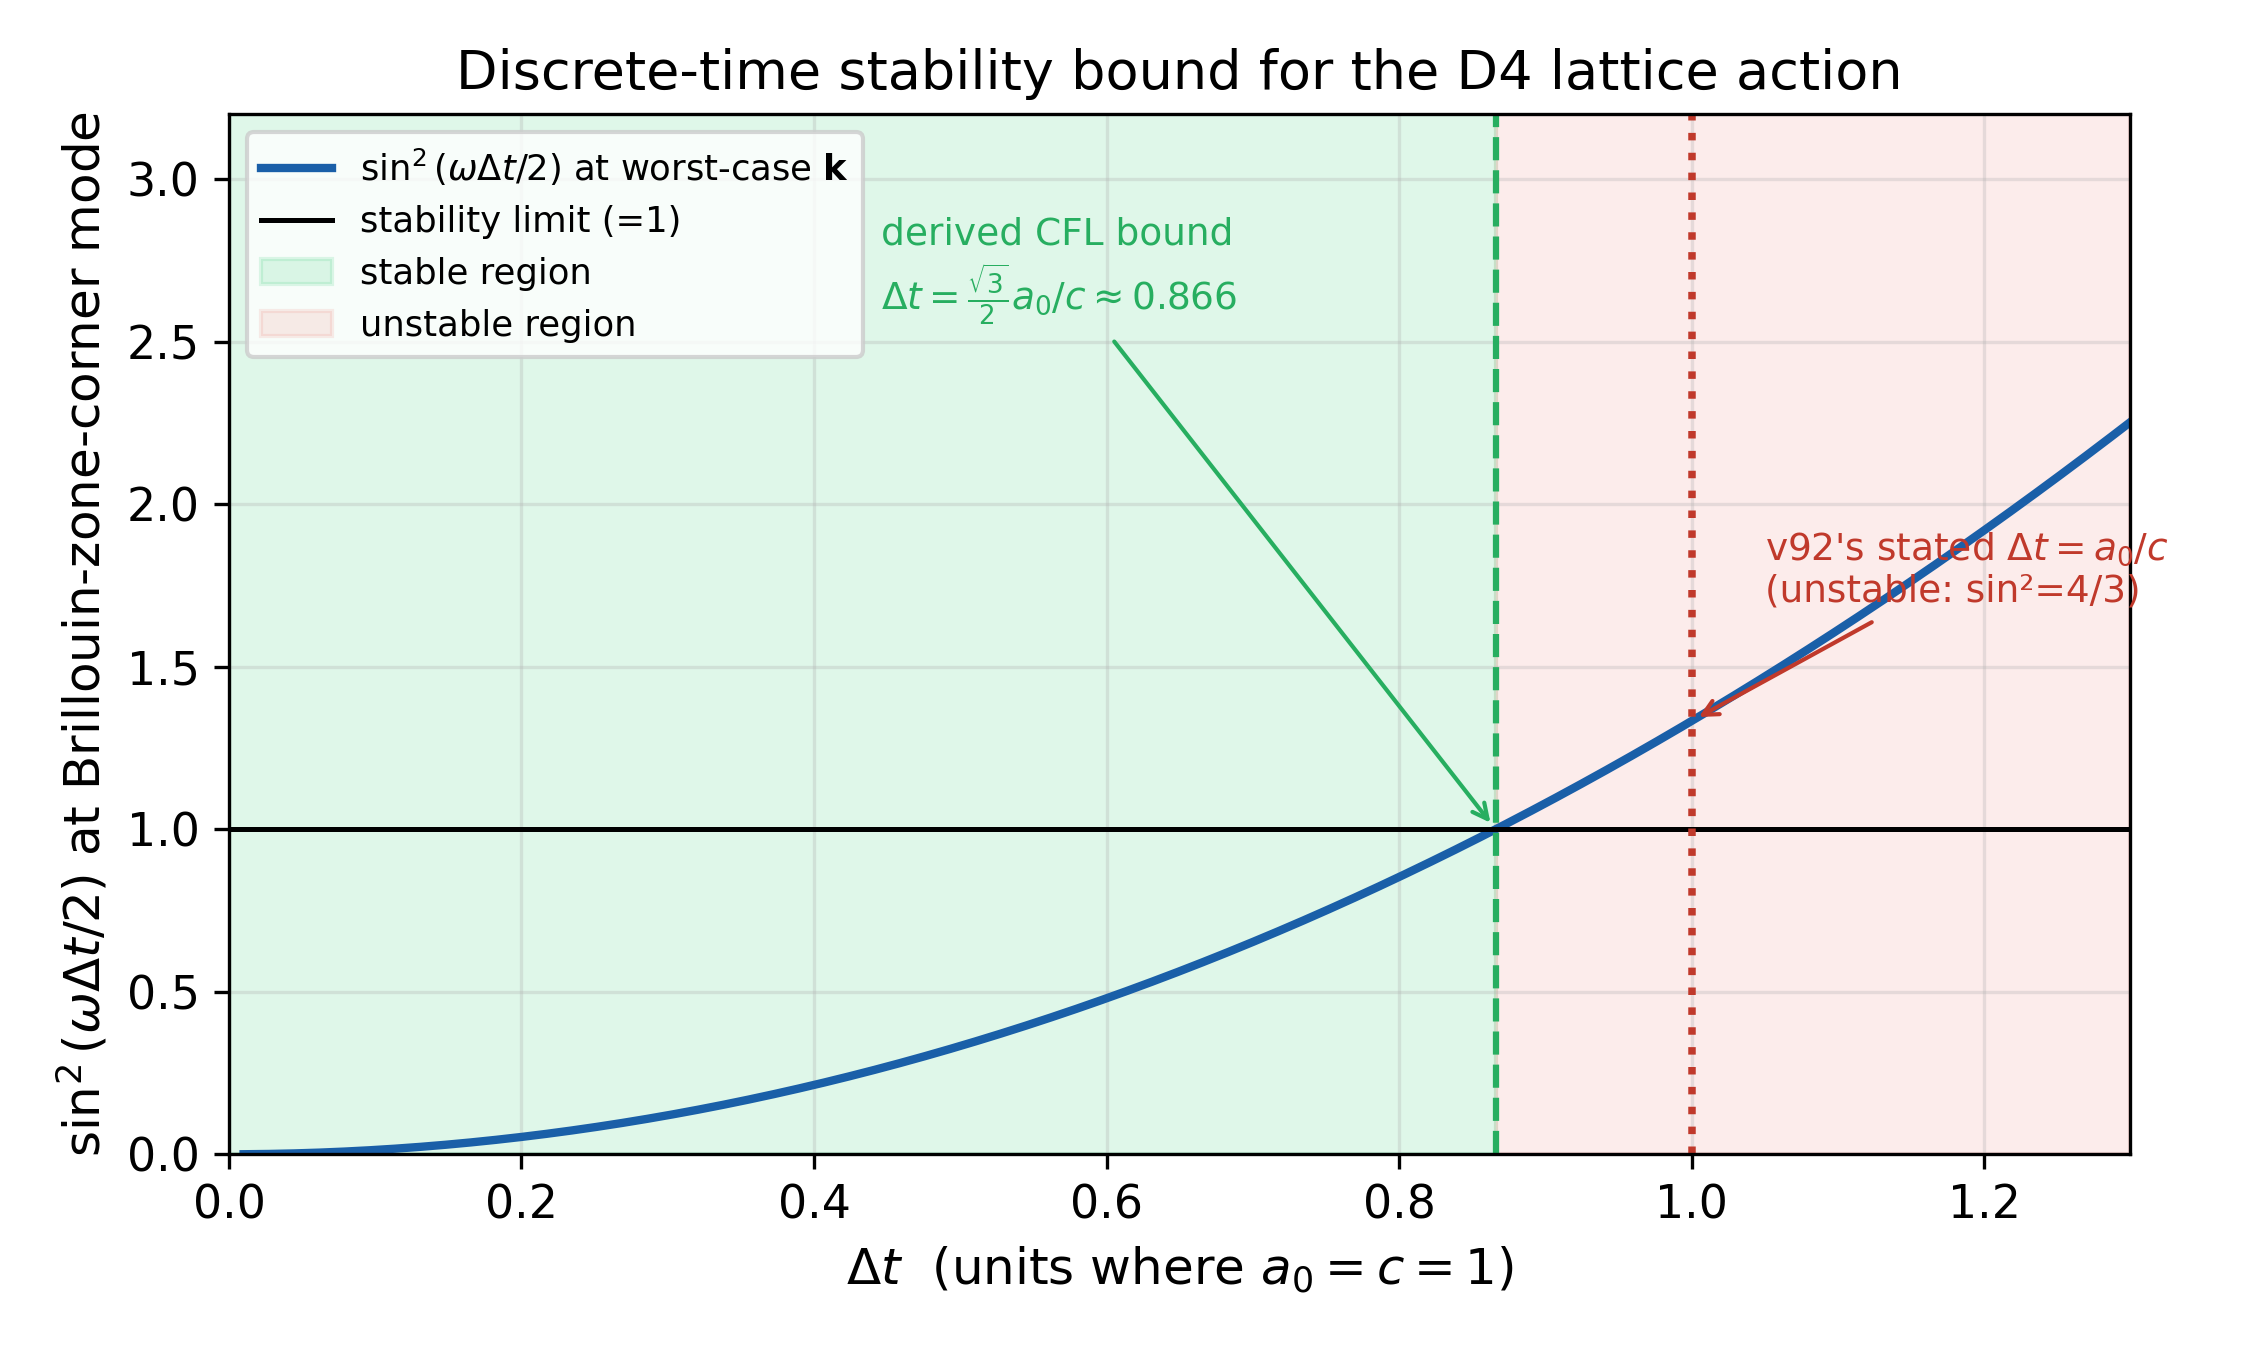
\includegraphics[width=0.8\linewidth]{figs/fig05.png}
\caption{The stability quantity $\sin^2(\omega\Delta t/2)$ at the worst-case Brillouin-zone mode, against the time step.}
\label{fig:cfl}
\end{figure}

\subsection{The non-relativistic limit}

Version 92 built a carrier $e^{-i\Omega_Ps\,T_P}$ with $T_P=2\pi/\Omega_P$, so that the carrier phase per step is exactly $2\pi$ and $e^{-i\theta s}=1$ for every integer $s$. Then the positive- and negative-frequency basis functions coincide, and the envelope decomposition is degenerate, not merely inaccurate.

With a genuine carrier angle $\theta\ne0,\pi$, write $\phi=\Psi\,e^{-i\theta s}+{\rm c.c.}$ with $\Psi$ slowly varying, and absorb the rest-mass term by choosing $\sin^2(\theta/2)=\Delta t^2\mu^2/(4M^*)$. Expanding the equation of motion \eqref{eq:eom} to first order in the time derivative of $\Psi$ gives
\begin{equation}\label{eq:schrod}
i\,\dot\Psi=-\frac{\Delta t\,J}{M^*a_0^2\sin\theta}\sum_{\alpha\in\Phi}\big[\Psi(n{+}\alpha,s)-\Psi(n,s)\big],\qquad m_{\rm eff}=\frac{M^*a_0\sin\theta}{c\,\Delta t}.
\end{equation}
To quantify where this holds, compare the exact dispersion \eqref{eq:disp} with the quadratic one, $\omega_{\rm quad}=\theta/\Delta t+|\mathbf{k}|^2/(2m_{\rm eff})$, which is its small-$\mathbf{k}$ tangent, and measure the relative error $|\omega_{\rm quad}-\omega_{\rm exact}|/\omega_{\rm exact}$ along $\mathbf{k}\parallel e_1$. We use units $a_0=c=M^*=1$ and $J=1/12$. The Brillouin zone of $D_4$ is a 24-cell whose facet centres lie at $a_0|\mathbf{k}|=\pi$, so $e_1$ reaches the zone edge at $a_0|\mathbf{k}|=\pi$. With $\mu\ne0$ the stability bound \eqref{eq:cfl} becomes $\Delta t_{\max}(\theta)=(\sqrt3/2)\cos(\theta/2)\,a_0/c$, and we work at that marginal value. The text fixes only $\theta\ne0,\pi$. Version 94 therefore chose a primary carrier, $\theta=\pi/2$, midway between the excluded values, so that $\Delta t=\sqrt{3/8}\,a_0/c$, and reported the range over $\theta\in[\pi/6,5\pi/6]$ beside it (Table~\ref{tab:nr}). The original statement, ``under $1\%$ for $a_0|\mathbf{k}|\lesssim0.3$'', is kept and qualified rather than replaced.

\begin{table}[htbp]
\centering
\begin{tabular}{lll}
\toprule
$a_0|\mathbf{k}|$ & error at $\theta=\pi/2$ & range for $\theta\in[\pi/6,5\pi/6]$\\
\midrule
0.02 & $1.6\times10^{-9}$ & $1.2\times10^{-10}$ to $1.5\times10^{-7}$\\
0.10 & $9.9\times10^{-7}$ & $7.6\times10^{-8}$ to $9.0\times10^{-5}$\\
0.30 & $7.9\times10^{-5}$ & $6.2\times10^{-6}$ to $6.0\times10^{-3}$\\
1.00 & $0.82\%$ & $0.076\%$ to $23\%$\\
$\pi$ (zone edge) & $41\%$ & $8.0\%$ to $248\%$\\
\bottomrule
\end{tabular}
\caption{Relative frequency error of the envelope (Schrödinger) approximation along $\mathbf{k}\parallel e_1$.}
\label{tab:nr}
\end{table}

\begin{figure}[htbp]
\centering
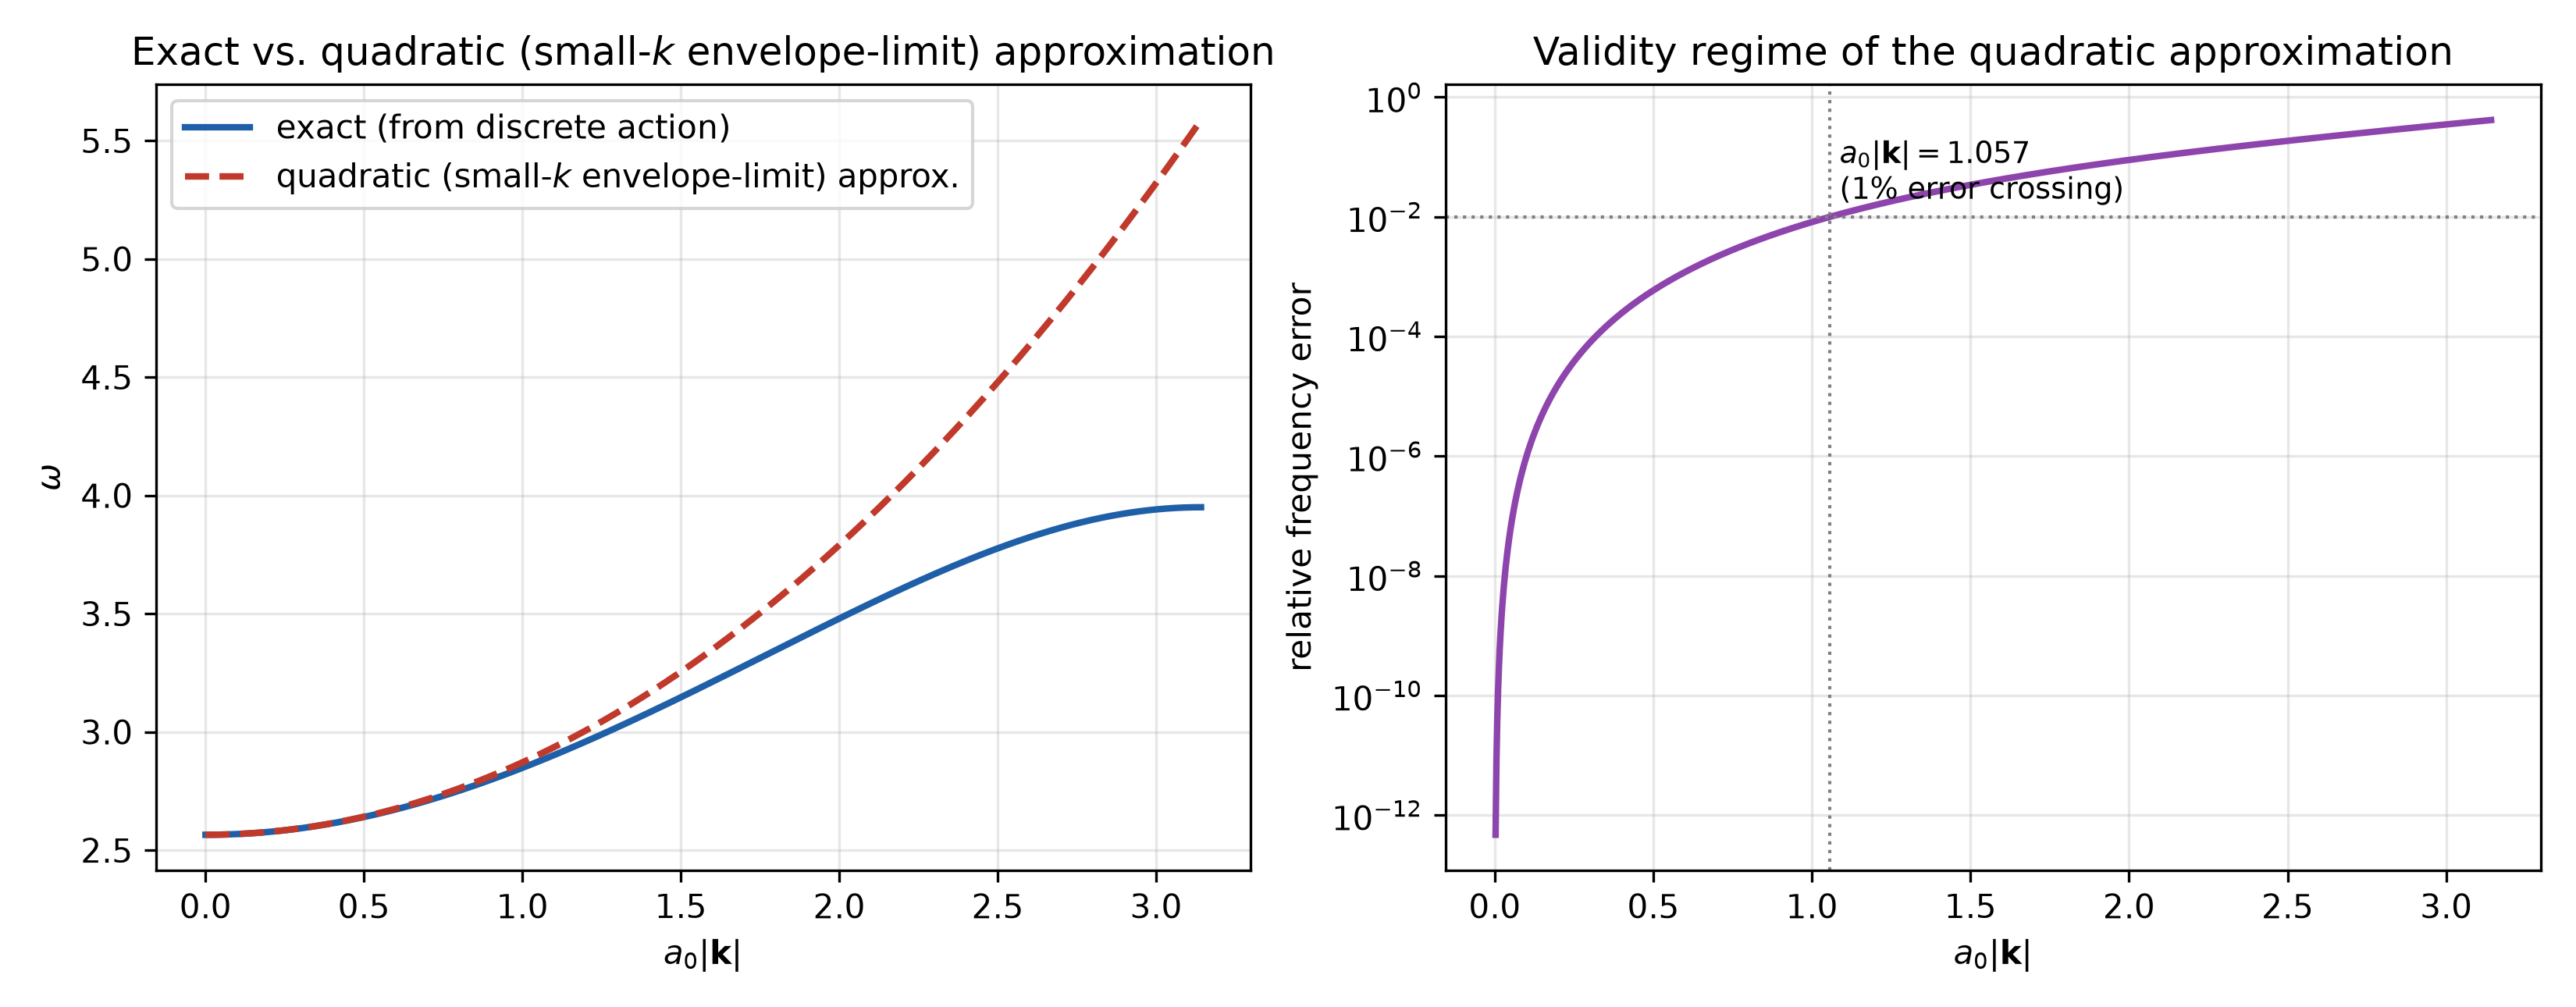
\includegraphics[width=0.8\linewidth]{figs/fig06.png}
\caption{Exact against quadratic dispersion along $\mathbf{k}\parallel e_1$ at $\theta=\pi/2$, $\Delta t=\sqrt{3/8}\,a_0/c$, and the relative error. The dotted lines mark the $1\%$ level, crossed at $a_0|\mathbf{k}|=1.057$.}
\label{fig:nr}
\end{figure}

At $\theta=\pi/2$ the approximation is good to $1\%$ for $a_0|\mathbf{k}|<1.057$, the error growing as $(a_0|\mathbf{k}|)^4$ at small $k$. The $1\%$ crossing moves with the free carrier angle, from $0.346$ at $\theta=\pi/6$ to $1.908$ at $\theta=5\pi/6$; at $\theta=\pi/12$ it is $0.173$. So the statement ``under $1\%$ for $a_0|\mathbf{k}|\lesssim0.3$'' holds throughout $\theta\in[\pi/6,5\pi/6]$ and fails for small carriers. The chosen $\theta$ is a reproducibility choice for these numbers; it does not correct anything in the earlier figure.

%===========================================================================
\section{Why four dimensions}\label{sec:four}
%===========================================================================

Rescale a field in $d$ dimensions, $\psi_\lambda(\mathbf{x})=\psi(\lambda\mathbf{x})$. Changing variables $\mathbf{y}=\lambda\mathbf{x}$ gives $d^dx=\lambda^{-d}d^dy$, each gradient brings a factor $\lambda$, and so
\begin{equation}\label{eq:derrick}
\int|\nabla\psi_\lambda|^2d^dx=\lambda^{2-d}I_{\rm grad},\qquad \int V(\psi_\lambda)\,d^dx=\lambda^{-d}I_{\rm pot},\qquad \int(\nabla^2\psi_\lambda)^2d^dx=\lambda^{4-d}I_{\rm curv}.
\end{equation}
Here $I_{\rm grad}$, $I_{\rm pot}$ and $I_{\rm curv}$ are the three integrals at $\lambda=1$. For a two-derivative energy $E(\lambda)=\lambda^{2-d}I_{\rm grad}+\lambda^{-d}I_{\rm pot}$, a static solution must be stationary under rescaling, $E'(1)=(2-d)I_{\rm grad}-dI_{\rm pot}=0$, that is $(d-2)I_{\rm grad}+dI_{\rm pot}=0$. For $d\ge3$ this forces $I_{\rm pot}<0$ unless the field is trivial. So with a non-negative potential there is no static localised solution, and where one exists it is unstable to rescaling. This is Derrick's theorem~\cite{ref15}, and it excludes stable solitons of a two-derivative scalar in four dimensions.

\lbl{Derivation} The four-derivative term scales as $\lambda^{4-d}$, which is $\lambda^0$ exactly when $d=4$. Four is the only dimension in which the curvature term of a Swift--Hohenberg substrate neither dominates nor disappears under rescaling, while the gradient and potential terms both contract (Figure~\ref{fig:scaling}). This is an argument for four dimensions independent of packing and kissing numbers, and it agrees with them: the dimension that hosts the optimal lattice~\cite{ref8} is the one in which the pattern-forming operator is marginal. It is a scaling statement, and it does not by itself construct a stable localised object.

\begin{figure}[htbp]
\centering
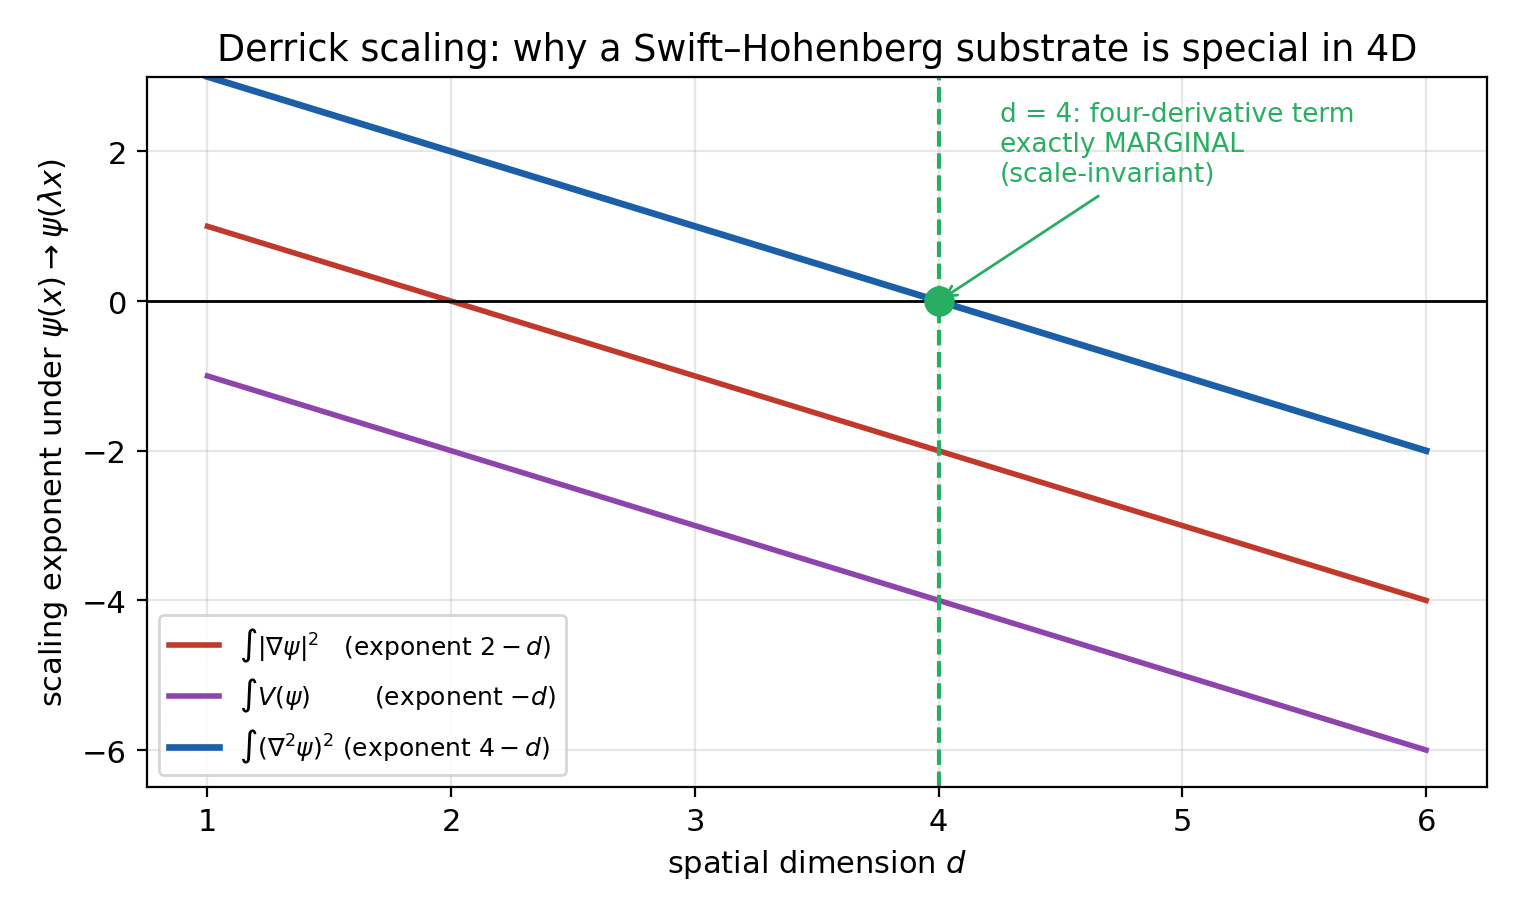
\includegraphics[width=0.8\linewidth]{figs/fig07.png}
\caption{Scaling exponents of the three terms against dimension. The four-derivative term is scale invariant exactly at $d=4$.}
\label{fig:scaling}
\end{figure}

%===========================================================================
\section{Algebraic structure}\label{sec:algebra}
%===========================================================================

\subsection{$\mathfrak{so}(8)$ cannot be the gauge algebra}

\lbl{Exclusion} We give two independent arguments.

The first concerns chirality. Every representation of a compact simple Lie algebra is self-conjugate exactly when $-1$ belongs to its Weyl group~\cite{ref21}. The Weyl group $W(D_n)$ consists of the permutations of $n$ coordinates combined with an even number of sign changes, so $|W(D_n)|=2^{n-1}n!$, which is $2^3\cdot24=192$ for $n=4$ and $2^4\cdot120=1920$ for $n=5$. The element $-1$ changes all $n$ signs, which is an even number exactly when $n$ is even. So $-1\in W(D_4)$ and $-1\notin W(D_5)$; constructing both groups by signed permutations and again by generating them from simple reflections gives the same orders and the same answers. Every representation of $\mathfrak{so}(8)$ is therefore self-conjugate, the three eight-dimensional representations are real and permuted by triality, and an algebra with only self-conjugate representations cannot give chiral fermion couplings. The Standard Model is chiral. This is also why $\mathfrak{so}(10)$, with $-1\notin W(D_5)$, has the complex $\mathbf{16}$.

The second concerns embedding. The Standard Model algebra $\mathfrak{su}(3)\oplus\mathfrak{su}(2)\oplus\mathfrak{u}(1)$ has rank $2+1+1=4$, equal to that of $\mathfrak{so}(8)$, so it could only appear as a maximal-rank subalgebra. By Borel and de Siebenthal~\cite{ref20} these are $\mathfrak{su}(4)\oplus\mathfrak{u}(1)$, $\mathfrak{su}(2)^{\oplus4}$ and $\mathfrak{su}(2)^{\oplus3}\oplus\mathfrak{u}(1)$. The towers of $\mathfrak{su}(2)$ cannot contain the simple rank-2 algebra $\mathfrak{su}(3)$. And $\mathfrak{su}(3)\oplus\mathfrak{su}(2)\not\subset\mathfrak{su}(4)$, since commuting faithful actions of the two factors need at least $3+2=5$ complex dimensions and $\mathfrak{su}(4)$ acts on $\mathbb{C}^4$.

The Pati--Salam algebra~\cite{ref22} $\mathfrak{su}(4)\oplus\mathfrak{su}(2)\oplus\mathfrak{su}(2)$ has rank $3+1+1=5>4$, so it is not a subalgebra of $\mathfrak{so}(8)$ by any route. The cascade $\mathfrak{so}(8)\to\mathfrak{g}_2\oplus\mathfrak{u}(1)\to$ Pati--Salam of version 92 also increases dimension, from $14+1=15$ to $15+3+3=21$, which no chain of subalgebras can do (Figure~\ref{fig:branch}).

\begin{figure}[htbp]
\centering
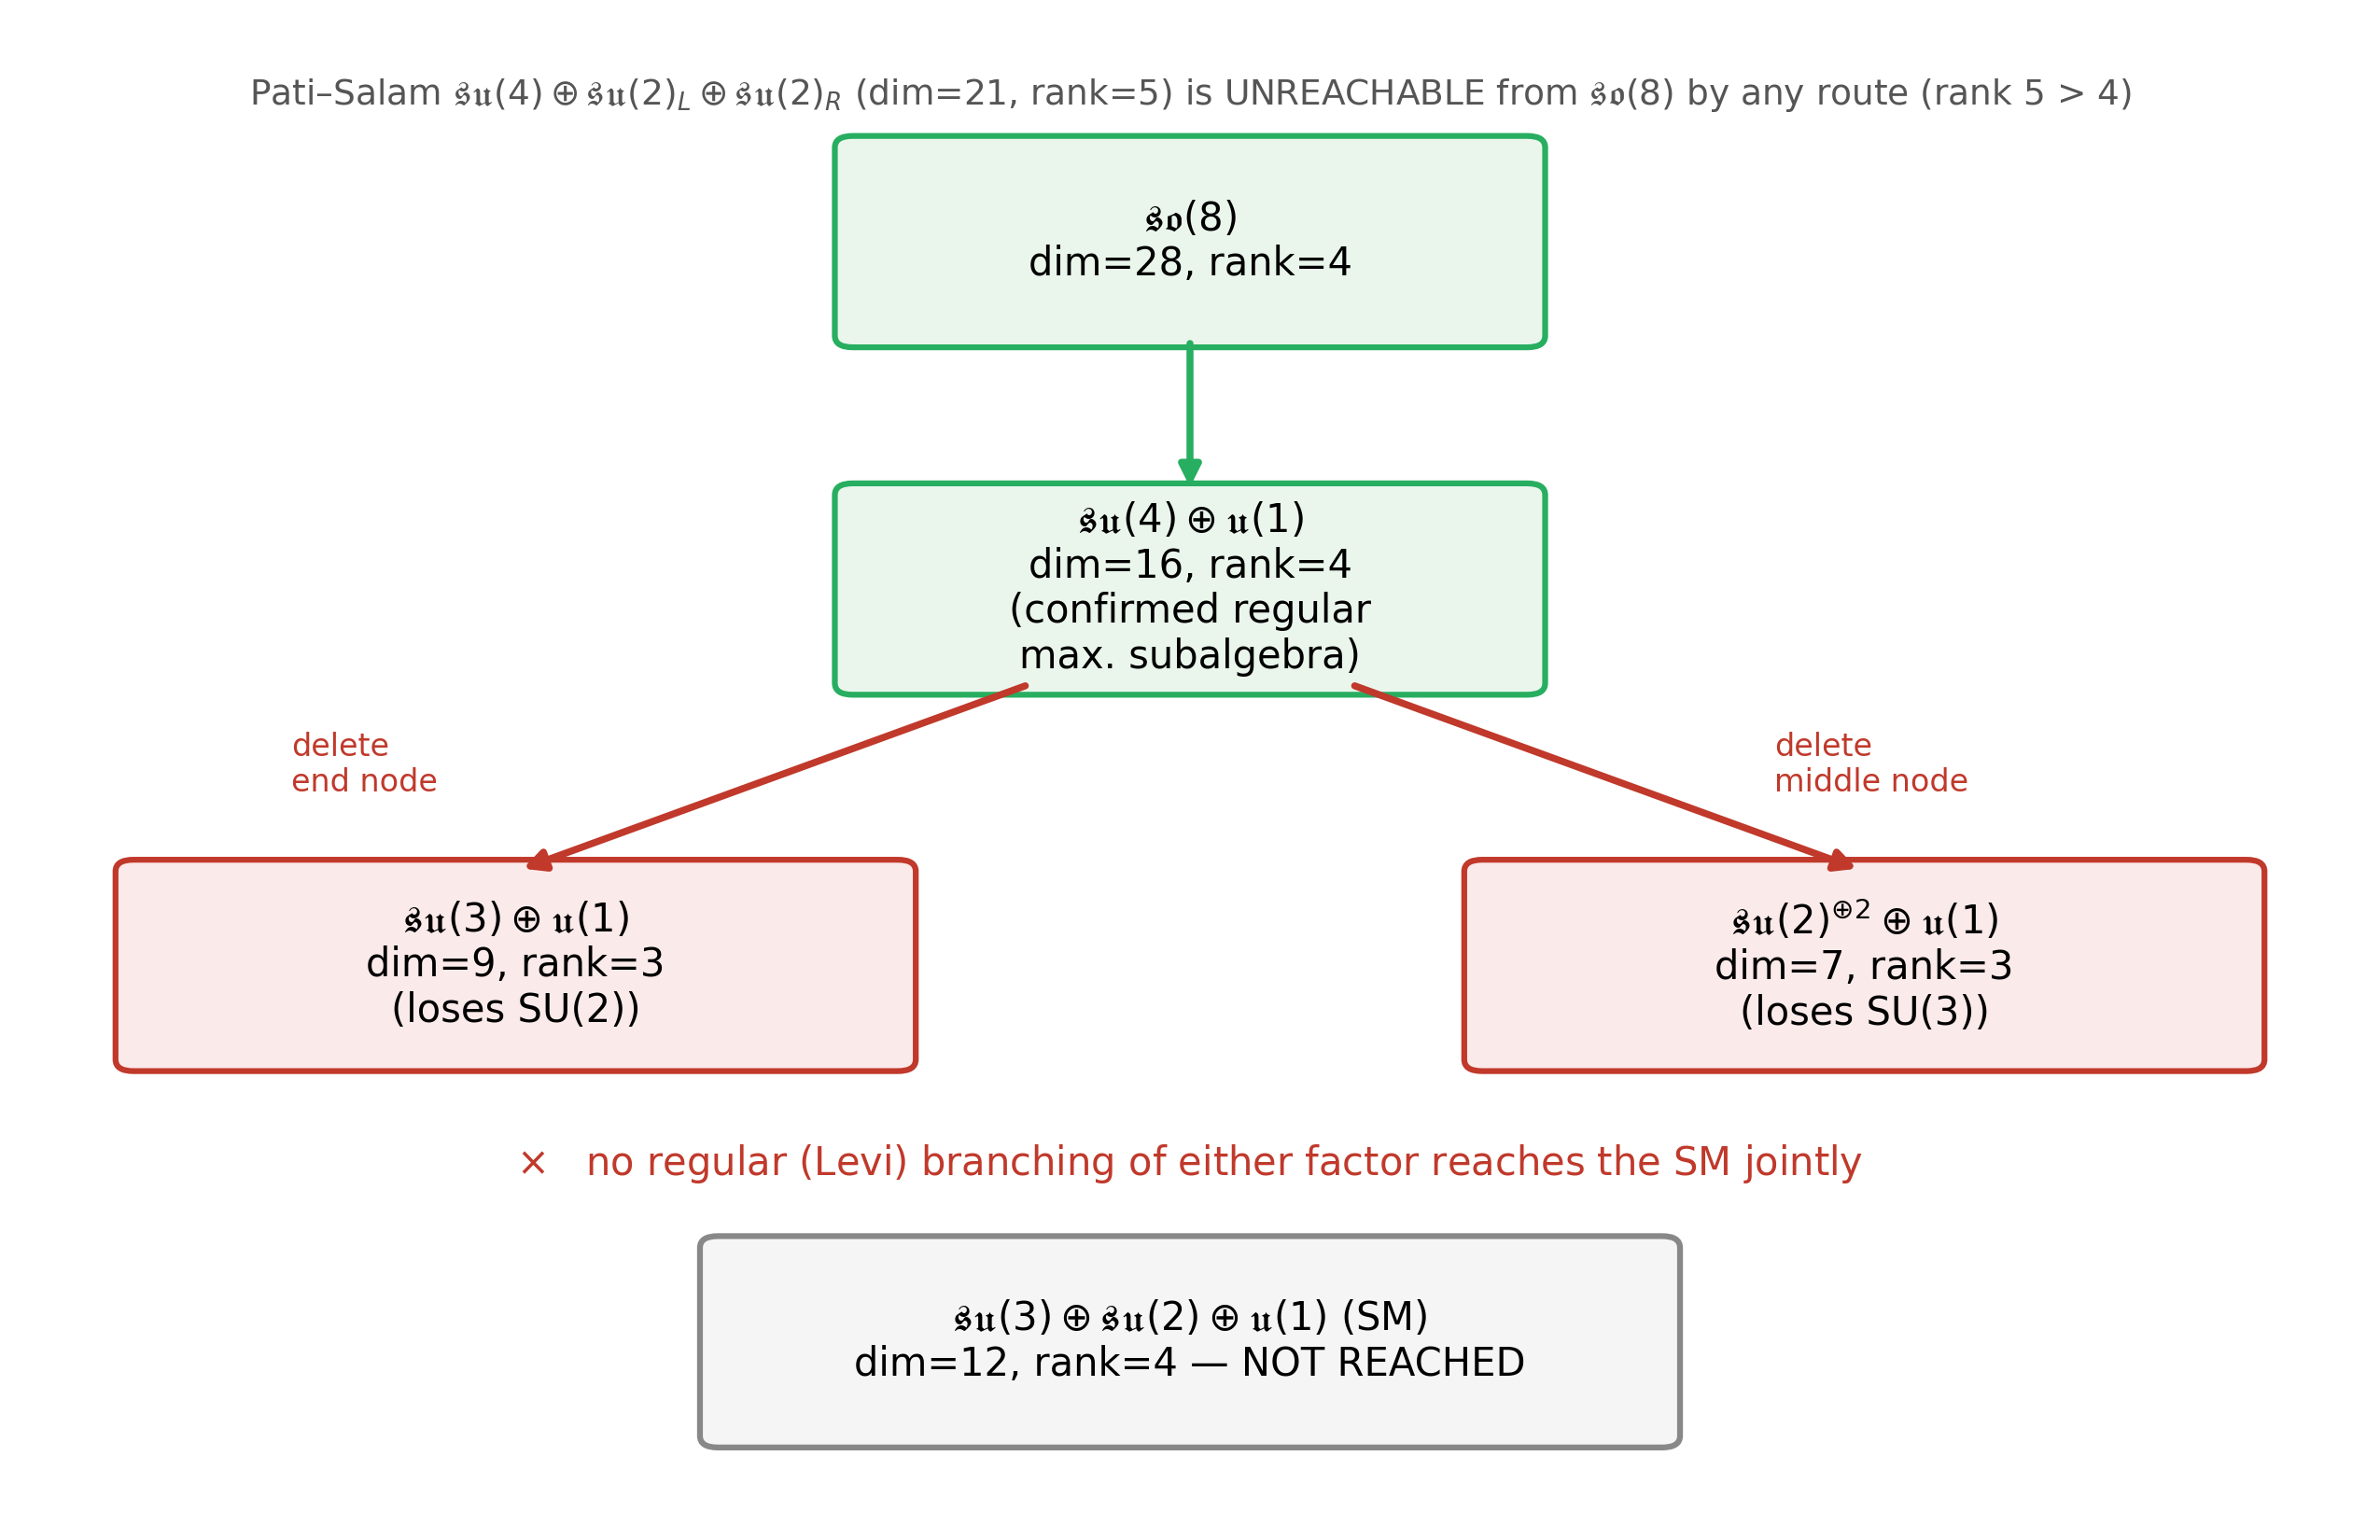
\includegraphics[width=0.8\linewidth]{figs/fig08.png}
\caption{Regular-subalgebra branchings of $\mathfrak{so}(8)$; neither route reaches the Standard Model.}
\label{fig:branch}
\end{figure}

\subsection{The phase sector carries no internal degrees of freedom}

\lbl{Derivation} A real $D_4$ density wave has $24$ modes in $12$ pairs $\pm\mathbf{g}$, so it has $12$ independent phases $\phi_a$. The cubic term of the free energy \eqref{eq:F} is lowest when $\phi_a+\phi_b+\phi_c\equiv0\pmod{2\pi}$ on every closed triad. There are $32$ unordered closed triads (the $192$ ordered triads of Section~\ref{sec:selection}, divided by the $3!=6$ orderings), and the $32\times12$ constraint matrix has rank $8$. That leaves $12-8=4$ free phases. A rigid translation $\mathbf{x}\to\mathbf{x}+\mathbf{a}$ shifts each phase by $\mathbf{g}\cdot\mathbf{a}$ and satisfies every triad constraint, because the three wavevectors of a triad sum to zero; translations span a $4$-dimensional subspace of the solutions. So $4-4=0$ phases remain once translations are removed. The order-parameter space is the torus $\mathbb{R}^4/\Lambda$, with no internal continuous symmetry, and its homotopy is $\pi_1=\mathbb{Z}^4$, $\pi_2=0$, $\pi_3=0$~\cite{ref23}. A single real scalar substrate can produce the $D_4$ pattern and dislocations. It cannot produce gauge fields or point defects. If the substrate is to carry either, it needs an internal space, and the question is which.

\subsection{The vertices of the 24-cell form a group}

Write the $24$ roots of $D_4^*$ of Section~\ref{sec:geometry} as quaternions: the eight units $\pm1,\pm i,\pm j,\pm k$ and the sixteen $(\pm1\pm i\pm j\pm k)/2$. These are the Hurwitz units~\cite{ref24}. Computing all $24^2=576$ products shows that the set is closed under quaternion multiplication and contains $1$ and all inverses. \lbl{Derivation} The vertex set of the 24-cell is the binary tetrahedral group $2T$~\cite{ref25}, a finite subgroup of the unit quaternions $SU(2)\cong S^3$. So the pattern supplies a candidate internal space, $S^3$, instead of requiring one to be posited, and it repairs the homotopy deficit, since $\pi_3(S^3)=\mathbb{Z}$.

The eight units $\pm1,\pm i,\pm j,\pm k$ form the quaternion group $Q_8$; it is closed, and every conjugate of an element of $Q_8$ by an element of $2T$ lies in $Q_8$, so $Q_8$ is normal. Hence $2T/Q_8\cong\mathbb{Z}_3$, with three cosets of eight elements. The $8+8+8$ splitting of the 24-cell is the coset decomposition of a group.

\subsection{The McKay correspondent of $2T$}

Conjugacy classes must be computed as conjugation orbits; trace and element order are too coarse and merge classes, which once gave five classes instead of seven. We find the irreducible representations of $2T$ from its class sizes and its abelianisation alone, without constructing them. The orbits have sizes $4,4,4,4,1,1,6$, summing to $24$. The number of irreducible representations equals the number of classes, seven; their dimensions square-sum to the group order; and $2T$ has abelianisation $\mathbb{Z}_3$, so exactly three are one-dimensional. The only solution is $\{1,1,1,2,2,2,3\}$, since $1+1+1+4+4+4+9=24$. These are the marks of the affine $E_6$ diagram, whose seven nodes carry $1,1,1,2,2,2,3$; affine $E_7$ has eight nodes and affine $E_8$ nine. \lbl{Derivation} By the McKay correspondence~\cite{ref3}, $2T$ corresponds to affine $E_6$. An earlier audit document identified it with affine $E_8$; that correspondent belongs to the binary icosahedral group of order $120$, and nothing built on that identification follows.

The longest element $w_0$ of the Weyl group acts as $-1$ for $D_4$ and not for $D_5$ or $E_6$. So $E_6$ passes the test that $\mathfrak{so}(8)$ fails: it has the complex $\mathbf{27}$~\cite{ref29}, and the rank chain $E_6\,(6)\supset SO(10)\,(5)\supset SU(5)\,(4)\supset{\rm SM}\,(4)$ is the standard non-increasing route~\cite{ref26,ref27,ref28}. One generation of Standard Model fermions fits in one $\mathbf{27}$. The Cartan matrix of $E_6$ has determinant $3$ and Smith normal form ${\rm diag}(1,1,1,1,1,3)$~\cite{ref30}, so the weight lattice modulo the root lattice is $P/Q\cong\mathbb{Z}_3$ (SymPy and Singular).

\begin{figure}[htbp]
\centering
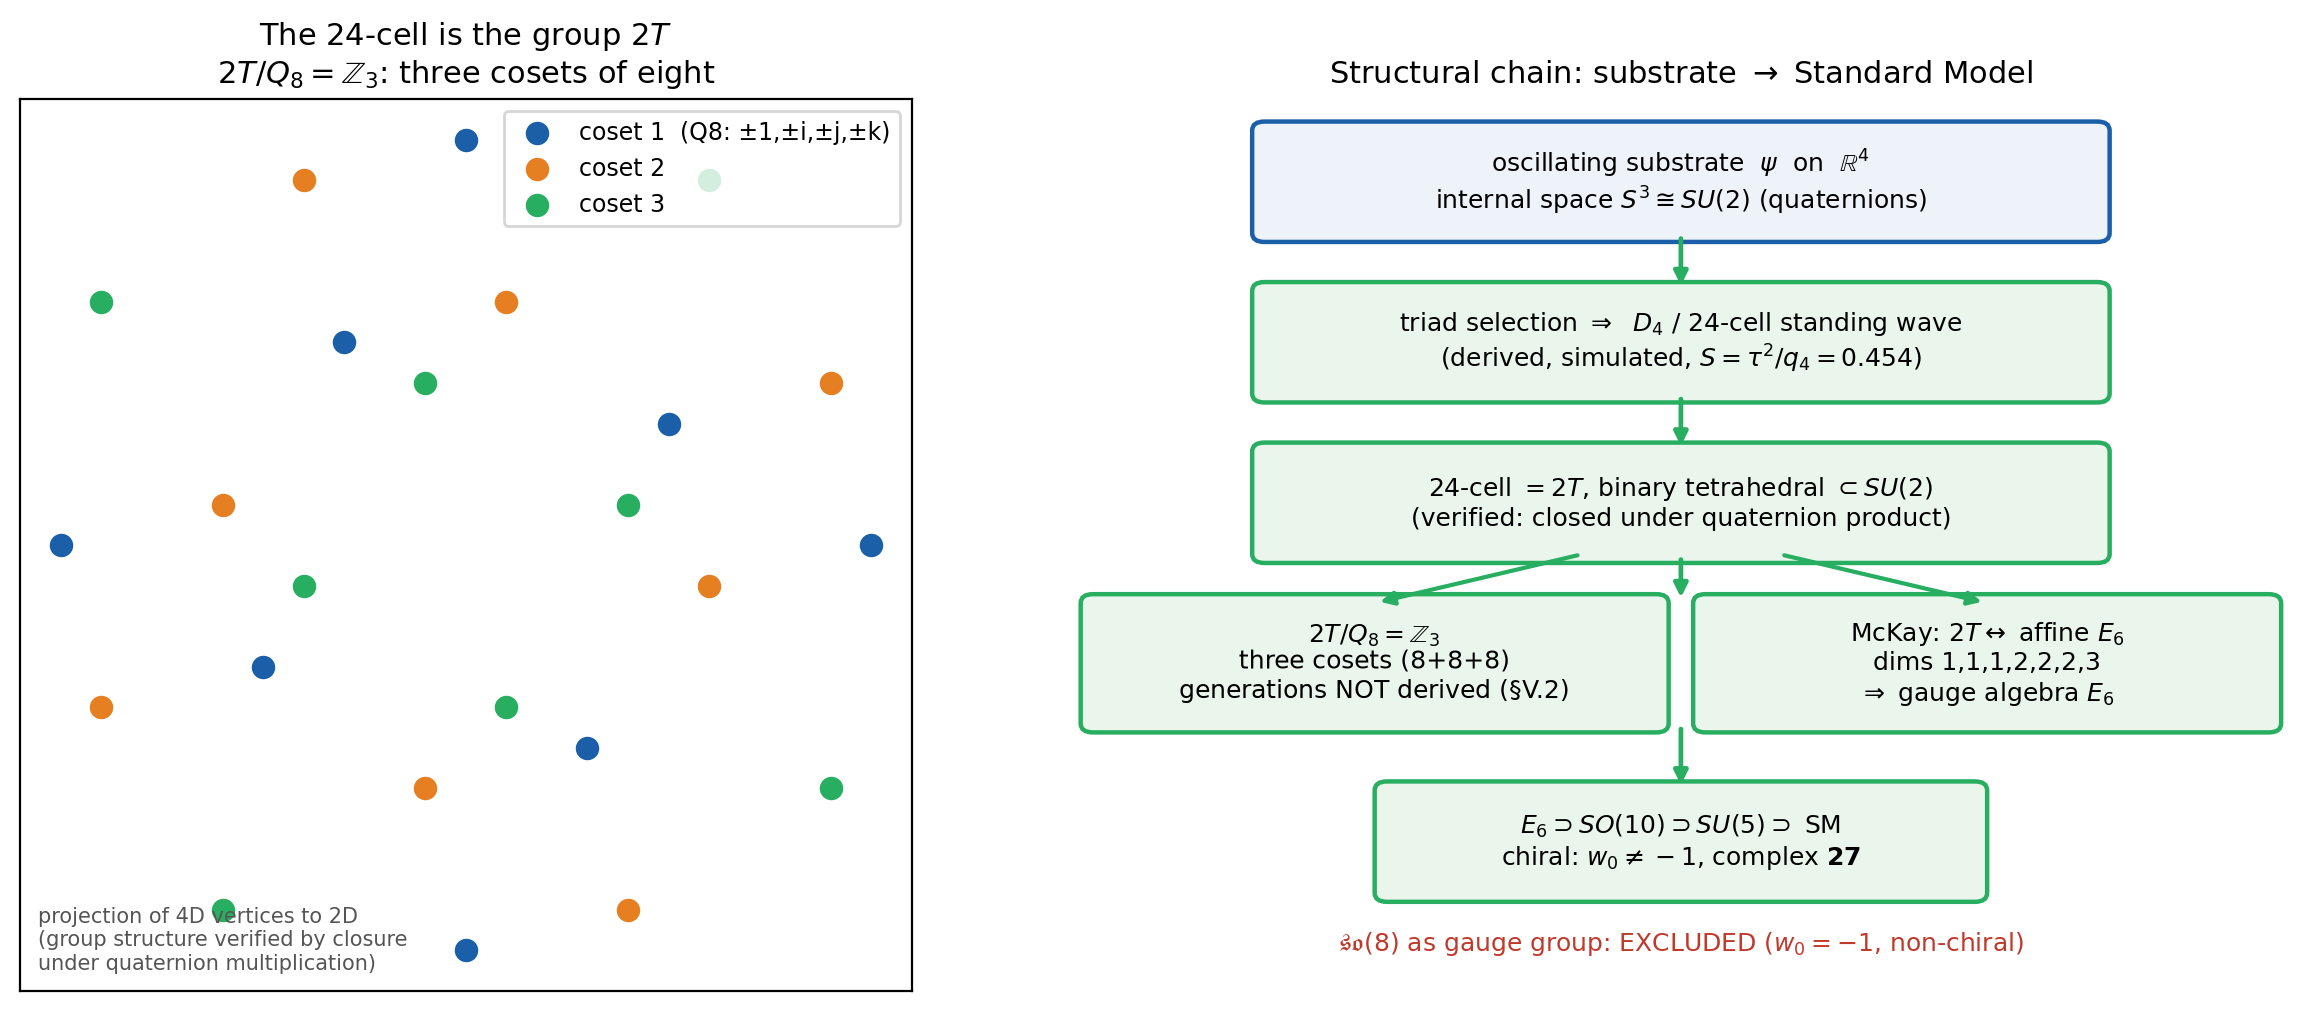
\includegraphics[width=0.85\linewidth]{figs/fig09.png}
\caption{Left: the 24 vertices of the 24-cell coloured by coset of $Q_8$ in $2T$. Right: the structural chain from the substrate to the Standard Model. The box reading ``gauge algebra $E_6$'' records a label, not a derived gauge algebra; no Yang--Mills term or Higgs sector is derived (gap G-A22). The box ``$2T/Q_8=\mathbb{Z}_3$'' records three cosets of eight; three generations are not derived from it (Section~\ref{sec:defects}).}
\label{fig:chain}
\end{figure}

\subsection{What the $E_6$ label means}

\lbl{Input} We adopt $E_6$ as the gauge-algebra label of the framework, read from the internal space $S^3\cong SU(2)$ through $2T$ and the McKay correspondence. The mathematics of this section is exact \grade{A}. Its physical reading as a gauge algebra is \grade{D}: no Yang--Mills kinetic term for an $E_6$ connection is derived from the dynamics of Section~\ref{sec:substrate}, and no Higgs sector breaking $E_6$ to $SU(3)\times SU(2)\times U(1)$ without light exotic relics is specified. What the label has in its favour is only that it was read off a pattern selected on separate dynamical grounds, rather than chosen to contain what was needed.

Two things are given up. Triality is no longer a generation mechanism, and $\mathfrak{so}(8)$ is no longer a gauge algebra. Triality survives as a symmetry of the defect classification: the point group of the $D_4$ lattice is $W(F_4)$ of order $1152$~\cite{ref6}, and $1152/192=6=|S_3|$, the extension of $W(D_4)$ by the triality automorphisms.

%===========================================================================
\section{Defects, generations and monopoles}\label{sec:defects}
%===========================================================================

\subsection{The defect spectrum}

With internal space $S^3$ the order-parameter space is $M=T^4\times S^3$, so $\pi_1(M)=\mathbb{Z}^4$, $\pi_2(M)=0$ and $\pi_3(M)=\mathbb{Z}$. In four spatial dimensions a defect of codimension $k$ is classified by $\pi_{k-1}(M)$~\cite{ref23}. Codimension-2 defects are dislocation sheets, classified by $\pi_1=\mathbb{Z}^4$, with Burgers vectors in the lattice $\pi D_4^*$; codimension-3 line defects are absent, since $\pi_2=0$; and codimension-4 point defects carry an integer charge in $\pi_3=\mathbb{Z}$. Point-like integer-charged objects of the kind the standing-wave picture needs therefore exist once the internal space is $S^3$, which they did not for a single real scalar. The elementary dislocation charges are the $24$ shortest vectors of $\pi D_4^*$, of length $|\mathbf{b}|=\pi$; for example $\mathbf{b}=(\pi/2)(1,1,1,1)$.

The dislocation coefficients were corrected in version 94 after outside checking, and the corrections stand. The Burgers lattice is $\pi D_4^*$, not $\pi D_4$, and there is one $W(F_4)$ orbit per shell of $D_4^*$ with $\|\mathbf{b}\|^2\le6$. The equilibrium ratio of edge to screw coefficients is $4/3$, not $2$; the earlier edge coefficient came from a non-equilibrium trial field and was $3/2$ too high. The corrected values are: elementary edge coefficient $0.490385\to0.326923$; $E/A$ at $R=20$, $0.899\to0.666$; edge critical radii rescaled by $\sqrt{2/3}$ ($16.62\to13.57$, $12.79\to10.44$, $23.91\to19.52$, $19.19\to15.67$); screw values unchanged. The bound state at $|\mathbf{b}|^2=4$ survives. At $R=20$ the edge split at $|\mathbf{b}|^2=10$ changes from no to yes ($E/E_{\rm elem}=3.0238$, $n_{\min}=3$, $R^*=19.52<20$, margin $0.79\%$, reproduced by a second route to $10^{-9}$), and the other verdicts at $R=20$ are unchanged \grade{B/F2; local edge leg incomplete pending a script rerun}. The stiffness used for these coefficients is the one-mode value $\lambda=\mu=256A^2$ of Section~\ref{sec:phonons}.

Defect realisation is contradicted in the tested setup (gap G-A11). A Volterra-defect prototype heals on relaxation, with $E/A=0.0013609$, about $9000$ times below the elastic prediction of about $12.5$ (about $6100$ times with the corrected edge coefficient), shows no $1/r^2$ field, and lives in a box whose largest radius $\pi\approx3.14$ is smaller than the analytic core scale $r_0\approx10.05$ or $7.10$. The sharpest remaining problem is a pinned, topologically protected defect in a box with $R_{\max}\gg r_0\approx10$.

\subsection{Generations are an input}

Does the $\mathbb{Z}_3=2T/Q_8$ produce three copies of the $\mathbf{27}$? Five mechanisms were tested, and none does.

The coset $\mathbb{Z}_3$ acts as a diagram automorphism: the three one-dimensional representations of $2T$ sit at the three mark-1 tips of the affine $E_6$ diagram, whose automorphism group of order $6$ permutes the arms. An automorphism permutes nodes; it does not multiply representations. The centre $\mathbb{Z}_3=P/Q$ grades representations: the $\mathbf{27}$ is in class $1$, the $\overline{\mathbf{27}}$ in class $2$ and the adjoint $\mathbf{78}$ in class $0$. Grading three different representations is not producing three copies of one. Anomaly cancellation imposes nothing, because the exponents of $E_6$ are $\{1,4,5,7,8,11\}$, there is no exponent $2$ and so no cubic Casimir, and the cubic anomaly vanishes for every representation~\cite{ref29}. The index route fails twice: on $S^3/2T$ the Dirac index vanishes by Lichnerowicz's theorem~\cite{ref31}, the metric having positive scalar curvature, and more basically it vanishes on every closed odd-dimensional manifold, because the index density is built from Pontryagin classes in degrees divisible by four~\cite{ref32}.

\lbl{Input} Three generations is an input. A symmetry that permutes cosets, a symmetry that grades representations and a multiplicity in the field content are three different things, and only the third would count. The 24-cell does split into three octets, and $E_6$ generations do come in threes, but the coincidence of the numbers is not a mechanism. The framework has not predicted three generations since $\mathfrak{so}(8)$ was excluded.

\subsection{Monopoles}

If $E_6$ is realised as a gauge group broken to a subgroup $H$ containing an unbroken $U(1)$, then $\pi_2(E_6/H)\cong\ker(\pi_1H\to\pi_1E_6)\supseteq\mathbb{Z}$, because $E_6$ is simply connected and $\pi_1(U(1))=\mathbb{Z}$, and stable magnetic monopoles exist~\cite{ref33}. Every chain ending in $SU(3)\times SU(2)\times U(1)$ is of this form. The claim of earlier versions that the framework has no monopoles is therefore retracted, and if the $E_6$ label is realised dynamically the framework inherits the monopole problem of unified theories, to be solved by dilution or by suppressed production.

%===========================================================================
\section{Reflection positivity}\label{sec:rp}
%===========================================================================

One reading of the framework (reading (A) of Section~\ref{sec:dimension}) takes the four-dimensional base to be Euclidean spacetime. A Euclidean field theory yields a relativistic quantum theory with positive norm only if its measure is reflection positive; this is the content of the Osterwalder--Schrader reconstruction~\cite{ref48,ref49}. We state the condition, then show that the Gaussian Swift--Hohenberg measure fails it. Version 94 made no positivity claim, so this section corrects nothing; it closes a question the reading left open (gap G-A27).

\subsection{The condition}

Pick a hyperplane, say $x_4=0$, and let $\theta$ be the reflection $(\mathbf{x}_\perp,x_4)\mapsto(\mathbf{x}_\perp,-x_4)$. For a Gaussian measure with covariance $C(\mathbf{x}-\mathbf{y})$, reflection positivity requires
\begin{equation}\label{eq:rpcond}
\langle\theta f,\,Cf\rangle=\int d^4x\,d^4y\;f(\theta\mathbf{x})\,C(\mathbf{x}-\mathbf{y})\,f(\mathbf{y})\ \ge0
\end{equation}
for every real test function $f$ supported in the half-space $x_4>0$. This is the simplest instance ($n=m=1$) of the Osterwalder--Schrader condition, and a single $f$ that makes the integral negative is enough to violate it.

\subsection{The disordered phase}

For $r>0$ the Gaussian part of \eqref{eq:F} about $\psi=0$ has covariance with Fourier transform
\begin{equation}\label{eq:Gs}
G(s)=\frac{1}{r+(q_0^2-s)^2},\qquad s=|\mathbf{k}|^2 .
\end{equation}
A reflection-positive, Euclidean-invariant scalar covariance has a Källén--Lehmann form $G(s)=\int\rho(dm^2)/(s+m^2)$ with a positive measure $\rho$, and every such function is non-increasing in $s$, since each integrand $1/(s+m^2)$ decreases in $s$ and $\rho$ is positive. Differentiating \eqref{eq:Gs}, however,
\[
\frac{dG}{ds}=\frac{2(q_0^2-s)}{\big(r+(q_0^2-s)^2\big)^2}>0\qquad\text{for }0\le s<q_0^2 ,
\]
so $G$ increases below the shell and has no such representation.

The failure can be exhibited directly. Fix the transverse momentum $\mathbf{k}_\perp$, put $a=q_0^2-|\mathbf{k}_\perp|^2$, and Fourier transform in $k_4$ alone:
\begin{equation}\label{eq:Gint}
\hat G(\mathbf{k}_\perp,x)=\int_{-\infty}^{\infty}\frac{\cos(k_4x)}{r+(a-k_4^2)^2}\,dk_4 .
\end{equation}
We evaluate \eqref{eq:Gint} by residues and then read off its sign.
The denominator vanishes where $k_4^2=a\pm i\sqrt r$. Let $z=\alpha+i\beta$ be the principal square root of $a+i\sqrt r$; then $\alpha,\beta>0$ for every real $a$ and every $r>0$, because $a+i\sqrt r$ lies in the open upper half-plane and its principal root in the open first quadrant. Squaring, $\alpha^2-\beta^2=a$ and $2\alpha\beta=\sqrt r$. The four poles are $\pm z$ and $\pm\bar z$, and the two in the upper half-plane are $z$ and $-\bar z$. Closing the contour there for $x>0$ and summing the two residues gives
\begin{equation}\label{eq:Ghat}
\hat G(\mathbf{k}_\perp,x)=\frac{\pi\,e^{-\beta x}\big(\alpha\cos\alpha x+\beta\sin\alpha x\big)}{2\alpha\beta\,(\alpha^2+\beta^2)} .
\end{equation}
We checked \eqref{eq:Ghat} against direct numerical quadrature (QUADPACK Fourier integration in SciPy~1.17.1) at four points, with agreement to about $2\times10^{-11}$, and the run record confirms it in SymPy, Wolfram Engine~15.0 and PARI/GP~2.15.2. At $x=\pi/\alpha$ we have $\cos\alpha x=-1$ and $\sin\alpha x=0$, so
\[
\hat G(\mathbf{k}_\perp,\pi/\alpha)=-\frac{\pi\,e^{-\beta\pi/\alpha}}{2\beta(\alpha^2+\beta^2)}<0,
\]
for every $\mathbf{k}_\perp$ and every $r>0$. At $a=8$, $r=0.1072$ this is $-1.6684$. The reflected kernel is negative at a reflected separation $2x_4=\pi/\alpha$, and a test function concentrated at that height, smeared in $\mathbf{x}_\perp$ and taken to the limit, makes the left side of \eqref{eq:rpcond} negative. The limit is controlled by a uniform bound: $|\alpha\cos\alpha x+\beta\sin\alpha x|\le|z|$, $2\alpha\beta=\sqrt r$ and $|z|^2=\sqrt{a^2+r}\ge\sqrt r$ give $|\hat G|\le\pi/(\sqrt r\,|z|)\le\pi r^{-3/4}$, and $\hat G$ is continuous in $\mathbf{k}_\perp$, so dominated convergence applies. Because $G$ depends only on $|\mathbf{k}|^2$, the measure is invariant under rotations, and every reflection hyperplane gives the same result.

\lbl{Exclusion} The Gaussian Swift--Hohenberg measure of the disordered phase on $\mathbb{R}^4$ is not reflection positive in any direction. The monotonicity, the absence of a Källén--Lehmann form and the sign at $x=\pi/\alpha$ are Lean kernel theorems; the residue identity \eqref{eq:Ghat} and the limiting argument are checked in computer algebra and by hand \grade{B, [MV]4K core / 4D Fourier step, F1/I1}.

\subsection{The crystal}

Around the relaxed $D_4$ crystal at $(r,\bar\psi)=(-0.35,-0.18)$, the Gaussian fluctuation measure was regularised on a lattice in the reflection direction (a nearest-neighbour time Laplacian, so that the positive control, a free massive field, is exactly reflection positive) and tested with site reflections along $e_4$ and along $(1,1,0,0)/\sqrt2$, and with link reflection along $e_4$. At every tested point the reflection matrix has a negative diagonal entry, so a single test function already violates positivity; the violation is of relative size $O(1)$, far above solver residuals of $10^{-11}$ or less. Positive and negative controls behave as they should on both routes \grade{F2/I1 at the ten points of the second route; F3/I1 elsewhere}. The scope is exactly this: the lattice-regularised measure, at the record point, in the tested directions. Nothing is inferred about the continuum crystal or the direction $(1,1,1,1)/2$.

\lbl{Exclusion} There is no Gaussian-level Osterwalder--Schrader route to a positive-norm Lorentzian theory from this functional: not about the disordered phase on $\mathbb{R}^4$, and not about the crystal for the lattice-regularised measure in the tested directions. A second branch, in which a negative-norm sector is identified and shown to decouple, has not been started, and no decoupling construction is known for this action. The sharpest remaining problem is the continuum statement for the crystal, for the operator $r+(q_0^2+\Delta)^2+w(\mathbf{x})$ with $w$ the periodic background of the crystal.

%===========================================================================
\section{The dimensional assignment}\label{sec:dimension}
%===========================================================================

\subsection{Three readings}

The framework has a four-dimensional base, an internal $S^3$ and an observed $3+1$-dimensional spacetime. Three readings of how these fit are mutually exclusive. In reading (A) the base is Euclidean spacetime and the Lorentzian signature arises dynamically. In reading (B) the base is four-dimensional space, $t$ is a physical time, one spatial direction is compactified, and Lorentz symmetry is to emerge from the phonons of the $D_4$ crystal; the cross-section of Section~\ref{sec:geometry} leaves fcc in the remaining three dimensions. In reading (C) the base is auxiliary and spacetime is emergent from defect dynamics. Version 94 said that the choice had to be made and could not be settled by further calculation. That second statement is overtaken: both (A) and (B) have now been tested by calculation.

\subsection{The decision and its reversal rule}

On the morning of November 25, 2026 the author adopted reading (B) as the working reading. Reading (A) was set aside because of the result of Section~\ref{sec:rp}, then available in preliminary form. Reading (C) was kept as the fallback. The decision was recorded together with a reversal rule fixed in advance. Reading (B) is dropped, and (C) becomes the working reading, if the phonon computation shows that no branch structure of the relaxed $D_4$ crystal, after compactification, gives a single massless sector with a common speed without tuning. Unequal speeds would not trigger the rule if one branch could be shown to be gapped or decoupled. Reading (A) is reinstated only if the fluctuation measure of the crystal is shown to be reflection positive in some direction.

\subsection{Outcome}

The phonon computation is Section~\ref{sec:phonons}. Its result, for the functional \eqref{eq:F} at the record point, is that the relaxed crystal has four gapless acoustic branches with two speeds, $c_L/c_T=1.731985$, and that compactifying one direction on any lattice circle keeps all four gapless at $q_\perp=0$ along the circle with the same two speeds. None of the four is gapped, since all are Goldstone modes of translations that a lattice-period compactification does not restore. None is decoupled, since the cubic coupling between the longitudinal and transverse modes is nonzero and no internal symmetry of $F$ separates them, the point group acting on wavevector and polarisation together. And Section~\ref{sec:phonons} showed that no stable isotropic solid has $c_L=c_T$, so no choice of the parameters of $F$, and no flow that stays in the stable solid phase, reaches a common speed. The trigger therefore fired, and the adjudicated ruling, made at about 16:30~UTC on November 25, upholds it \grade{B/F2/I1, scoped}. The reflection-positivity test of Section~\ref{sec:rp} found no positive direction, so the condition for reinstating (A) did not occur.

The present state is as follows. Reading (B) is dropped. Reading (C) is the working reading, and no construction of it exists; ``working reading'' means only that it is the one not yet excluded. Reading (A) is not reinstated and has no Gaussian-level positivity route. The negative results are scoped to the substrate as specified: the functional \eqref{eq:F}, the Hessian dynamics in the limit $\gamma\to0$ (with the conserved, inertial dynamics checked on one route), lattice-translation circles and a mirror orbifold, and the record point. Three ways out lie outside that scope, and each changes the theory rather than the calculation: a flow out of the solid phase, a new field, or a new term in $F$. At the damping $\gamma=1.2$ of the simulations, the long-wavelength modes are overdamped in any case.

Two consequences follow for later work. The three follow-up tests that were written for reading (B), namely radius selection for the compact direction, the Kaluza--Klein spectrum as a falsifier, and the higher Lorentz-violating operators, no longer test a working reading and have to be re-scoped or retired; the Kaluza--Klein numbers of Table~\ref{tab:kk} and the coefficients $\xi_6$ are kept as properties of the substrate, not predictions. And the direction of the programme now depends on a choice between constructing reading (C) and changing the substrate, which is a decision about the theory and is not made in this paper.

\subsection{Related gaps}

Whether a common emergent speed exists for the substrate as specified (gap G-A29) is closed with a negative answer, scoped as above. Whether Lorentz violation is naturally suppressed (gap G-A28) is overtaken: in the phonon sector the violation is not small but of order one at leading order, a species-dependent mismatch of light cones, isotropic at order $q^2$, with direction dependence entering only at order $q^4$ through $P_6$. No separation of scales removes a leading-order mismatch of cones. The causality of the dispersive modes (gap G-A30) is open. Nothing in this paper shows that the full retarded response of the substrate has support inside a light cone, and there is reason to expect the opposite: at large wavenumber the dispersion of the wave equation \eqref{eq:dw} behaves as $\omega\sim q^2$, so the principal symbol $\omega^2-|\xi|^4$, with $(\omega,\xi)$ dual to $(t,\mathbf{x})$, is of plate type rather than hyperbolic. That argument has been made once and not independently checked, so we state it as the sharpest form of the open question and not as a result.

%===========================================================================
\section{Predictions}\label{sec:predictions}
%===========================================================================

The framework makes the following predictions, each stated before the data it would be tested against. They are predictions about the substrate model, and under the present state of Section~\ref{sec:dimension} none of them is a prediction about observed spacetime.

Triad phase locking. For a real field with $u>0$ the cubic term is lowest when $\phi_1+\phi_2+\phi_3\equiv0\pmod{2\pi}$ on every closed triad. This distinguishes a genuine $D_4$ standing wave from a superposition of modes that merely lie on the right shell. In simulation the locking order parameter was $0.26$ against a maximum of $1$, which is real but incomplete locking, as expected of a defected state in a small box; a larger volume should drive it towards $1$.

The band of baseline tension. The full $24$-mode pattern is the global minimum only for $\bar\psi$ in a band along the order--disorder boundary, of the size given by the band fraction \eqref{eq:band}, and only for $q_0$ tuned onto the shell. Outside either condition a lower-symmetry pattern, or none, results.

The validity of the envelope limit. The frequency error of the Schrödinger limit of Section~\ref{sec:legacy} is below $1\%$ for $a_0|\mathbf{k}|\lesssim0.3$ when $\theta\in[\pi/6,5\pi/6]$, and degrades as in Table~\ref{tab:nr}.

The stability bound. Every discrete implementation of the site-field dynamics needs $\Delta t\le(\sqrt3/2)a_0/c$.

Isotropy to fourth order. The nearest-neighbour $D_4$ coupling produces no anisotropic quartic term; anisotropy enters at sixth order, or through next-nearest-neighbour couplings. This is a prediction of absence. Version 94 presented it as the leading statement about Lorentz violation. The phonon computation shows that the leading violation in the crystal is a different and larger one, the isotropic mismatch $c_L\ne c_T$ of Section~\ref{sec:phonons}, so the prediction of absence concerns only the directional part.

The defect spectrum. Dislocation sheets with Burgers vectors in $\pi D_4^*$, integer-charged point solitons, and no line defects.

Monopoles. Predicted, not excluded, if the $E_6$ label is realised as a broken gauge group (Section~\ref{sec:defects}).

%===========================================================================
\section{Verification}\label{sec:verification}
%===========================================================================

\subsection{Independent recomputation}

The load-bearing results of Sections~\ref{sec:geometry}--\ref{sec:algebra} were reproduced from scratch by a separate implementation: the moment identities, the resonance maximum of $24$, the stability bound, the dispersion identity, the cross-section, the Weyl-group orders and the position of $-1$, the quaternion computations and the identity $u_{\rm eff}=u-3v\bar\psi$. The attractor of Section~\ref{sec:stability} was reproduced: seeded at $A^*=0.0776$, the state is stationary to about $10^{-5}$, Model~B holds the amplitude to four figures, and the Model~A drift to $\bar\psi=+0.00087$ with rms modulation $0.4206$ matches. The causal test of Section~\ref{sec:sim} was reproduced at the level of mechanism, with the numbers given there. The same review proposed two findings that did not survive checking, the attribution of the free-energy gap to the baseline (Section~\ref{sec:stability}) and a count of $16$ periodic images of the resonance maximum instead of $32$ (Section~\ref{sec:geometry}); its underlying point, that ``unique'' must mean ``unique modulo the lattice'', was adopted. A reported late instability of the conserved scheme at $t\gtrsim12$ did not recur in our scheme over the same horizon, and we regard it as specific to that implementation.

\subsection{Formal verification}

The Lean~4 development accompanying version 93.1 contains no \texttt{sorry}, \texttt{axiom}, \texttt{admit} or \texttt{native\_decide}. Its nine theorems cover the isotropy identities for a general wavevector, the dispersion identity, the stability bound, the selection criterion and its rationals, the identity for $u_{\rm eff}$, the cross-section and $-1\in W(D_4)$, and it builds end to end (\texttt{lake build} exit $0$, $3101$ jobs, all eight modules).

In this edition $23$ further claims, C01--C23, are Lean~4.34.0 kernel theorems against Mathlib commit \texttt{5ed2965}, proved with the tactic \texttt{decide +kernel} and using no axioms beyond \texttt{propext}, \texttt{Classical.choice} and \texttt{Quot.sound}, rebuilt from scratch and replayed by an independent checker; the sources are in the repository under \texttt{verification/lean-gb6/}. They cover the shell counts of Table~\ref{tab:S4} and the ratio $496/423$ (C01--C10), the cosine fingerprint of the root and dual shells (C11, whose dual half is proved in the verifier's supplementary file), the shell counts and resonance maximum set on the $16^4$ grid (C12--C16, C22), the count $H=911{,}040$ (C17), the one-mode and stability algebra (C18--C21) and the test points of $\Psi$ (C23) \grade{B, [MV]4K F1/I1}. Three carry conditions. C17 holds under the reading of $H$ as the number of ordered zero-sum $6$-tuples of shell vectors, since the definition is not printed. C21 depends on the bracket maximum $32$, now itself a kernel theorem, and on the reading of the prefactor of \eqref{eq:disp}. C23 holds under the convention $D_4=\{\sum y_i\ \text{even}\}$ with the shell taken as the minimal vectors of $D_4^*$. The $0.1\%$ margin of Section~\ref{sec:geometry} remains a floating-point statement. The lemmas of Section~\ref{sec:rp} are likewise kernel theorems.

\subsection{The literature}

Two independent literature sweeps found no work, other than the author's own, that cites or discusses this framework; two research-network records show zero citations, and full-text checks of five candidate works found no mention of the author \grade{B, scoped}. The universal negative is not established; the statement is about the sweeps. Two comparisons promised to outside collaborators (grain locking and a spectral threshold) cannot be made because the files never arrived, and nothing is claimed about them.

%===========================================================================
\section{Retractions from version 92}\label{sec:retractions}
%===========================================================================

Each claim in Table~\ref{tab:retract} is withdrawn for a stated reason.

\begin{table}[htbp]
\centering
\small
\begin{tabular}{p{0.33\linewidth}p{0.15\linewidth}p{0.44\linewidth}}
\toprule
version 92 claim & status & reason\\
\midrule
anisotropy coefficient $\xi_2=-1/384$ & retracted & the $D_4$ fourth moment is exactly isotropic; the value comes from a hypercubic stand-in, whose own substitution gives $-1/768$\\
$\mathfrak{so}(8)\to\mathfrak{g}_2\to$ Pati--Salam & retracted & dimension rises $15\to21$ and rank $3\to5$\\
$SO(8)$ as gauge group & retracted & non-chiral, $-1\in W(D_4)$\\
three generations from triality & retracted & five mechanisms closed; now an input\\
$\Delta t=a_0/c$ and $\Delta t=T_P$ & retracted & both violate the bound \eqref{eq:cfl}\\
Schrödinger emergence & corrected & the original carrier is degenerate; replaced in Section~\ref{sec:legacy}\\
Lorentzian signature from $i^2=-1$ & retracted & complex amplitudes are used in Euclidean field theory too; they do not select a signature\\
Einstein equations from elasticity & retracted & an analogy, not a derivation\\
absence of monopoles & retracted & inconsistent with $E_6$ broken to a group with a $U(1)$\\
Higgs value $v_0$, $A_3$ mass and widths, CKM & retracted & computed in an excluded framework, with separate arithmetic errors\\
``zero empirical calibration'', ``100\% closure'' & retracted & not defensible in any version\\
$\alpha^{-1}=137+1/(28-\pi/14)$ as derived & downgraded & the arithmetic is exact, the derivation absent \grade{D}\\
normalisation $R=2589$ & downgraded & the subtraction of $3$ is not forced by any displayed symmetry\\
\bottomrule
\end{tabular}
\caption{Claims withdrawn from version 92.}
\label{tab:retract}
\end{table}

The $\alpha$ ansatz deserves its numbers. Since $\pi/14=0.2243994753$, we have $28-\pi/14=27.7756005247$ and $1/27.7756005247=0.0360028219$, so the ansatz gives $\alpha^{-1}=137.0360028219$. The CODATA 2022 value is $137.035999177(21)$. The difference, $3.645\times10^{-6}$, is $173.6$ standard uncertainties. The ansatz is a numerical coincidence at the level of five figures and is excluded at the level of the measurement.

%===========================================================================
\section{Status and open problems}\label{sec:status}
%===========================================================================

We measure the distance to a complete theory against an explicit bar of eight tiers, T0 to T7, written before this edition and kept with the programme records. No tier is met in full. We go through them in order and give, for each open item, the sharpest problem it has been reduced to.

\subsection{Foundations (T0)}

What the theory is (T0.1) was decided as reading (B) and then, by the rule fixed with it, moved to reading (C) (Section~\ref{sec:dimension}). Reading (C) has no construction, so T0.1 is again open in substance. A well-posed classical dynamics (T0.2) is partial: the manuscript's requirement of conserved dynamics and its equations now agree, but existence and uniqueness for the conserved inertial equation have not been studied. A defined quantum theory (T0.3) is partial and lattice-scoped. A UV-regulated finite periodic four-dimensional lattice can be quantised canonically, with the quadratic sector checked on two engines \grade{F2/I1} and the propagator at $v>0$ on one \grade{F3/I1}. The Euclidean route is closed at Gaussian level by Section~\ref{sec:rp}, so a continuum quantum theory, if there is one, must come from a Hamiltonian construction or from a decoupling argument not yet found. The record itself (T0.4) is consistent except where stated: the values $11.85\%$ and $11.90\%$ are recorded as not reproducible, and the corrections of Appendix~\ref{app:corrections} are applied.

\subsection{Emergence of $D_4$ (T1)}

Selection by the theory's own dynamics (T1.1) is partial and box-scoped. Patterned recovery is established; from noise, the result holds in the barrier-free sliver at $L=3\pi$ with high probability (Section~\ref{sec:gd3}); at the metastable operating point no noise quench reached $D_4$. The sharpest problem is the trend of the basin fraction with the box size, starting at $L=5\pi$. What fixes $\bar\psi$ and $q_0$ (T1.2) is open, with no mechanism. Under conserved dynamics $\bar\psi$ is an initial datum, so the fine-tuning objection becomes a question about initial conditions, which is a weaker charge but not an answer, and the tuning of $q_0$ onto the shell is a separate condition. Stability and nucleation in infinite volume (T1.3) are partial: the full-field barrier \eqref{eq:barrier} is known, while continuum stability over the whole Brillouin zone and the nucleation rate are open, as stated in Sections~\ref{sec:stability} and~\ref{sec:nucleation}.

\subsection{Gauge structure (T2)}

A dynamical gauge field (T2.1) is not obtained. The $E_6$ identification (T2.2) is mathematics at grade A with a physical reading at grade D. Breaking to $SU(3)\times SU(2)\times U(1)$ (T2.3) has not been started, and the literature indicates that every breaking of $E_6$ costs either light exotic states or tuning. Monopoles (T2.4) follow if the breaking is realised (Section~\ref{sec:defects}).

\subsection{Matter (T3)}

The substrate is a single real scalar and contains no fermion (T3.1); skyrmions from a single real scalar are excluded by the homotopy of Section~\ref{sec:algebra}. Three generations (T3.2) is an input. Anomaly cancellation (T3.3) holds automatically for any number of $\mathbf{27}$s and so constrains nothing. Masses, mixings and the Higgs value (T3.4) must be restarted; nothing from the excluded framework is carried forward.

\subsection{Spacetime and gravity (T4)}

Lorentzian signature (T4.1) is open, and every transfer of a known mechanism fails. The one-loop mechanism of Greensite and of Carlini and Greensite~\cite{ref41,ref42} requires more fermionic than bosonic degrees of freedom in a one-loop effective potential; it was re-derived exactly and gives $D=4$ uniqueness for massless non-supersymmetric fields, but the substrate has no fermions. The classical mechanisms~\cite{ref17,ref18} use a clock field, and no classical mechanism is known that selects the signature for a single-scalar Swift--Hohenberg $D_4$ substrate without a tuned clock field. The argument of version 92 from $i^2=-1$ is invalid. Emergent Lorentz invariance with a common light speed (T4.2) is excluded for the phonon route, for the functional as specified (Section~\ref{sec:phonons}), and has no live route in any of the three readings as constructed. The Einstein equations (T4.3) are not derived. Identifying the metric with the local impedance tensor of the substrate is the standard analogue-gravity construction~\cite{ref16}: waves on a slowly varying background define an effective metric, with geodesic bending and horizons, but that metric obeys the substrate's own equation of motion and not $G_{\mu\nu}=8\pi T_{\mu\nu}$~\cite{ref19}. Recovering the field equations, diffeomorphism invariance, the Bianchi identity, universal coupling to conserved stress-energy and the two graviton polarisations is a separate programme. Newton's constant and the post-Newtonian parameters (T4.4) are open. One external fact bears on any varying-$G$ proposal: lunar laser ranging gives $\dot G/G=(4\pm9)\times10^{-13}\ {\rm yr}^{-1}$~\cite{ref50}, which excludes Dirac's large-number hypothesis.

\subsection{Quantum consistency (T5)}

Unitarity (T5.1) is established only on the regulated lattice. Reflection positivity (T5.2) fails at Gaussian level (Section~\ref{sec:rp}); a negative-norm sector that decouples has not been looked for. The continuum limit and renormalisation (T5.3) are open: the one-loop determinant needed for a nucleation rate diverges in four dimensions, and a prescription has to be chosen. Reproducing entanglement and the violation of Bell inequalities~\cite{ref37} from a classical substrate needs either nonlocality or superdeterminism~\cite{ref38} (T5.4). That is a boundary of the approach, not a gap in it.

\subsection{Predictions and independence (T6, T7)}

None of the predictions of Section~\ref{sec:predictions} has been tested against data (T6.1), and there is no discriminating prediction (T6.2); the coefficients $\xi_6$ and the Kaluza--Klein gaps are numbers of the model, without a physical scale. Kernel-checked statements exist for the geometric and combinatorial core and for the positivity lemmas (T7.1). Independence at level I3 or better (T7.2) is not met: every check in this paper was run by the author's own pipeline, and the strongest independence reached is I1 (Appendix~\ref{app:grades}).

%===========================================================================
\section{Assessment}\label{sec:assessment}
%===========================================================================

The verification cycles since version 92 have produced a framework that is different from the one they started with, and smaller.

What was removed was removed for cause: an anisotropy coefficient that cannot be derived from the stated lattice, a gauge algebra excluded by a Weyl-group computation, time steps that violate their own stability bound, a generation count resting on a confusion of symmetry with multiplicity, and the claimed absence of monopoles. In this edition two further things go. The first is the hope of reading the four-dimensional base as Euclidean spacetime with a positive-norm continuation, which fails at Gaussian level. The second is the hope that the phonons of the crystal supply an emergent light cone, which fails because a stable isotropic solid has two sound speeds. Both were stated as hopes in version 94 and are now settled by computation.

What remains has been computed, checked against known limits, simulated where simulation was possible, and in one instance corroborated by an unrelated published result. The selection criterion $S=\tau^2/q_4$ singles out $D_4$ in four dimensions with an exact margin $496/423$; the full $24$-mode state is a dynamical attractor of conserved dynamics in a definite band of baseline tension; the transition into it is first order, with a full-field barrier of $119.06$ in the units of the free energy \eqref{eq:F}; and the vertex set of the pattern is a group whose McKay correspondent is affine $E_6$. These are statements about a pattern-forming field in four dimensions, and they are the part of the programme that is solid.

The position, then, is this. IRH is a well-posed programme about the emergence of a high-symmetry structure from an oscillatory substrate, with a verified geometric core and a list of open problems that Section~\ref{sec:status} states one by one. It is not a unified theory, and after this edition it is further from being a theory of spacetime than version 94 suggested: no reading of the base as spacetime survives as constructed. The central claim, that a high-symmetry discrete structure can be selected dynamically rather than imposed, is supported. Whether that structure has anything to do with the world is the question the programme now has to face directly.

\appendix

%===========================================================================
\section{Record of corrections}\label{app:corrections}
%===========================================================================

Errors found over the verification cycles, including the author's own, are recorded here because each changed a conclusion or a reader's ability to check one.

Version 94 listed twenty. An audit document's confirmation of $\xi_2=-1/384$ did not survive recomputation, since the $D_4$ fourth moment is isotropic and the document's own substitution gives $-1/768$. A wavepacket test gave erratic errors of $30$--$200\%$, traced to a phase-sensitive metric and excessive momentum spread. A scan suggesting that $A_4^*$ beats $D_4$ applied a near-threshold criterion outside its regime and counted $D_4$ against its own dual. A simulation meant to put two shells in degeneracy put the resonant wavenumber on a third shell; that shell had no triads and produced lamellae, which confirmed the mechanism negatively. Sub-patterns within a shell were left out of the free-energy comparison, and the simulation exposed the omission, leading to $\bar\psi$ as control parameter. Trace and order merged conjugacy classes of $2T$, giving five classes instead of seven. A computation returned class $0$ for all six fundamental weights of $E_6$, inconsistent with a nontrivial centre, and was corrected by Smith normal form. A free-energy scan mixed normalised $\tau,q_4$ with a raw mode count and gave $63.8\%$ instead of about $11.6\%$. An explicit Euler step against an operator reaching $6\times10^4$ overflowed. A script printed a pre-written conclusion that its own output contradicted; the explanation, a sub-critical seed at a first-order transition, was found by rejecting the printed text. Power fractions were computed without subtracting the mean. Seeds were normalised by peak rather than per-mode amplitude, suppressing them by a factor $24$. A conserved time step of $0.2$ diverged, because the explicit nonlinear term is multiplied by $k^2$ up to $256$. The phase diagram used bare $r$ while simulations used detuned $q_0$. The box length and shell normalisation, the excess-over-uniform convention, the competitor shell of the causal test and the table convention for $A_4$ and $A_4^*$ were not stated, which made results irreproducible though correct. The Burgers lattice was $\pi D_4^*$ and not $\pi D_4$, and the edge-to-screw factor $4/3$ and not $2$. And the ``$K=6$'' study did not widen the $A_4^*$ band, because the solver caps $|\mathbf{k}|^2\le64$; it was a grid check, and whether the trap survives a genuinely wider band is unverified.

This edition adds the following. The band value is fixed at $758/6561=11.5531\%$ under the definition of Section~\ref{sec:band}; the values $11.85\%$ and $11.90\%$ of the earlier record cannot be reproduced and are withdrawn. The uniform free-energy density $1.0333364$ includes the term $\tfrac12q_0^4\bar\psi^2$, which earlier text omitted from the formula while including it in the number. The envelope barrier $550.93057$ and the ODE value $555$ are saddles of a radially restricted model and are not the barrier of the field; the full-field value is \eqref{eq:barrier}, lower by a factor of about $4.6$. The barrier-to-noise ratio of about $34$ refers to the restricted model; for the full field it is about $7.3$. The statement that the transition question ``is not resolvable by further calculation'' is overtaken (Section~\ref{sec:dimension}). The long-wavelength ratio $3.016$ is $c_L^2/c_T^2$ at $|\mathbf{q}|=0.02$, not the $\mathbf{q}\to0$ limit $2.99977$. The stiffness $1.54058921$ agrees with the one-mode value $256A^2$ at the one-mode amplitude; the relaxed crystal has $\mu=1.54465$ and $\lambda=1.54447$. The leading Lorentz violation of the crystal is the isotropic mismatch of sound speeds, not directional anisotropy. The chosen carrier angle $\theta=\pi/2$ in Table~\ref{tab:nr} is presented beside the original statement rather than replacing it. A question raised about the prefactor $\Delta t^2\,2J/(4M^*a_0^2)$ of the dispersion relation \eqref{eq:disp}, that it was wrong by a factor of $2$, came from a text-extraction error that read the exponent in $a_0^2$ as a factor; the equation is unchanged from version 93.1 and needs no erratum. In the references, the DOI of Gürsey, Ramond and Sikivie ends in \texttt{90417-2}, not \texttt{90417-6}, and the arXiv identifier \texttt{math/0607446}, which belongs to Cohn and Kumar, has been removed from the entry for Elitzur, Karni and Rabinovici. The Lean system description occupies pages 378--388 of the CADE-25 proceedings, with DOI ending \texttt{21401-6\_26}, not pages 26--48 with \texttt{\_2}, and the Mathlib paper occupies pages 367--381 of the CPP 2020 proceedings, not 30--46.

%===========================================================================
\section{Methods and reproducibility}\label{app:methods}
%===========================================================================

All computation was done on a Google Cloud virtual machine of type \texttt{n2-custom-24-98304} (24 virtual CPUs, 96~GB memory), with a local machine used only to control it. Symbolic algebra used SymPy~1.14.0~\cite{ref36} under Python~3.11.16; the Euler--Lagrange variation, the dispersion reduction, the ordered-branch solution, the effective coefficients and the elastic tensor were obtained symbolically. Numerical work used NumPy~2.4.6, SciPy~1.17.1~\cite{ref11} (L-BFGS-B, differential evolution, QUADPACK) and mpmath~1.4.1. Polynomial systems and Cartan-matrix invariants were computed in Singular~4.4.1 and msolve~0.9.5; independent checks of identities, of the phonon spectra and of Lie-algebra results used Wolfram Engine~15.0 (Weyl groups generated from simple reflections, a construction independent of the signed-permutation one used in Python), and invariant counts for $W(F_4)$ used GAP~4.12.1. Formal proofs are in Lean~4.34.0 with Mathlib at commit \texttt{5ed2965256430c3649e86755f9576b54eca72435}~\cite{ref34,ref35}. Field simulations used a semi-implicit pseudo-spectral scheme~\cite{ref10} on periodic grids, with the linear operator treated implicitly in Fourier space and time steps chosen separately for conserved and non-conserved dynamics; a second, binary-independent route in C with FFTW was used for the selection, barrier and phonon results graded F2. Higher-order mode counts used FFT convolution on a $32^4$ grid, checked against brute-force enumeration at third and fourth order. Group computations for $2T$ were exhaustive. Random seeds were fixed. Every figure was generated from the computation it reports.

Every result above the level of a single computation followed one protocol. Before a test was run, its parameters, pass and fail conditions and kill condition were written down and frozen. A known-false claim was planted in each verifier's checklist, and a verification counted only if the verifier caught it. An independent verifier re-derived the result with its own code, seeds and, for grade F2, a different binary, without access to the author's scripts. An adjudicator then compared the two against the frozen conditions and assigned the grade. Grades are never raised by restatement; a result is quoted here at the grade the adjudication gave it. The scripts, logs and checksums for each test are in the repository and the run records, and the recomputations behind the numbers of this paper are in \texttt{programme/v95/validation/}.

%===========================================================================
\section{Grades and labels}\label{app:grades}
%===========================================================================

Each result carries one of six labels. A derivation follows from the stated premises by explicit steps. A prediction is a consequence stated before it is tested. A calibration fixes a parameter by a datum. An input is an assumption the framework does not derive. An exclusion is a negative result. An open problem is stated with the sharpest form to which it has been reduced.

Grades follow the HLRE~v5.1 protocol. For empirical and computational support (Track~E) the grades are A, protocol-frozen, quantitatively successful and tested at independence I4 (or I3 with a discriminating comparison fixed in advance); B, strong constrained support; C, a plausible constrained hypothesis; and D, exploratory. For mathematical and formal claims (Track~F) the levels are F1, machine-checked or independently re-derived with a closed ledger of premises; F2, supported by one independent human or machine route; and F3, a single-route computation or one verified only by artificial means. In this programme a numerical result is given F2 only when two routes independent in code and in binary agree. Independence levels run from I0, the same data used in construction and in the check, through I1, a new analysis sharing selection choices with the original (which includes automated pipelines sharing inputs or sources), I2, a held-out observable under a frozen protocol or a re-derivation by a verifier who had not seen the original, and I3, an independent team, dataset or instrument, to I4, independent replication with an adversarial or competing-model comparison. All checks in this paper were run within the author's own pipeline, so I1 is the ceiling. The tag [MV]4K marks a statement whose load-bearing part is a Lean kernel theorem, and [MV]4D one whose load-bearing part is a closed-ledger derivation by hand or computer algebra.

The paper uses standard mathematical and physical terms (Lie algebra, gauge field, discrete Laplacian, dispersion relation, order parameter) rather than relabellings of them, so that every result can be checked against the literature on spherical designs, Lie algebras and pattern formation.

%===========================================================================
\begin{thebibliography}{99}
\small
\bibitem{ref1} S. Alexander and J. McTague, Should all crystals be bcc? Landau theory of solidification and crystal nucleation, \textit{Phys.\ Rev.\ Lett.} \textbf{41} (1978) 702--705, doi:10.1103/PhysRevLett.41.702.
\bibitem{ref2} J. Swift and P. C. Hohenberg, Hydrodynamic fluctuations at the convective instability, \textit{Phys.\ Rev.\ A} \textbf{15} (1977) 319--328, doi:10.1103/PhysRevA.15.319.
\bibitem{ref3} J. McKay, Graphs, singularities, and finite groups, \textit{Proc.\ Sympos.\ Pure Math.} \textbf{37} (1980) 183--186.
\bibitem{ref4} P. C. Hohenberg and B. I. Halperin, Theory of dynamic critical phenomena, \textit{Rev.\ Mod.\ Phys.} \textbf{49} (1977) 435--479, doi:10.1103/RevModPhys.49.435.
\bibitem{ref5} P. Delsarte, J. M. Goethals and J. J. Seidel, Spherical codes and designs, \textit{Geom.\ Dedicata} \textbf{6} (1977) 363--388, doi:10.1007/BF03187604.
\bibitem{ref6} J. H. Conway and N. J. A. Sloane, \textit{Sphere Packings, Lattices and Groups}, 3rd ed., Springer, New York, 1999.
\bibitem{ref7} O. R. Musin, The kissing number in four dimensions, \textit{Ann.\ of Math.} \textbf{168} (2008) 1--32, doi:10.4007/annals.2008.168.1.
\bibitem{ref8} A. Korkine and G. Zolotareff, Sur les formes quadratiques positives, \textit{Math.\ Ann.} \textbf{11} (1877) 242--292, doi:10.1007/BF01442667.
\bibitem{ref10} L. N. Trefethen, \textit{Spectral Methods in MATLAB}, SIAM, Philadelphia, 2000.
\bibitem{ref11} P. Virtanen et al., SciPy 1.0: fundamental algorithms for scientific computing in Python, \textit{Nature Methods} \textbf{17} (2020) 261--272, doi:10.1038/s41592-019-0686-2.
\bibitem{ref12} S. Bernstein, Sur les fonctions absolument monotones, \textit{Acta Math.} \textbf{52} (1929) 1--66, doi:10.1007/BF02592679.
\bibitem{ref13} H. Cohn, J. H. Conway, N. D. Elkies and A. Kumar, The $D_4$ root system is not universally optimal, \textit{Experiment.\ Math.} \textbf{16} (2007) 313--320, arXiv:math/0607447.
\bibitem{ref14} D. de Laat, N. Leijenhorst and C. de Muinck Keizer, Optimality and uniqueness of the $D_4$ root system, arXiv:2404.18794 (2024).
\bibitem{ref15} G. H. Derrick, Comments on nonlinear wave equations as models for elementary particles, \textit{J.\ Math.\ Phys.} \textbf{5} (1964) 1252--1254, doi:10.1063/1.1704233.
\bibitem{ref16} C. Barceló, S. Liberati and M. Visser, Analogue gravity, \textit{Living Rev.\ Relativ.} \textbf{14} (2011) 3, doi:10.12942/lrr-2011-3.
\bibitem{ref17} S. Mukohyama and J.-P. Uzan, From configuration to dynamics: emergence of Lorentz signature in classical field theory, \textit{Phys.\ Rev.\ D} \textbf{87} (2013) 065020, arXiv:1301.1361.
\bibitem{ref18} J. Kehayias, S. Mukohyama and J.-P. Uzan, Emergent Lorentz signature, fermions, and the Standard Model, arXiv:1403.0580 (2014).
\bibitem{ref19} L. Sindoni, Emergent models for gravity: an overview of microscopic models, \textit{SIGMA} \textbf{8} (2012) 027, arXiv:1110.0686.
\bibitem{ref20} A. Borel and J. de Siebenthal, Les sous-groupes fermés de rang maximum des groupes de Lie clos, \textit{Comment.\ Math.\ Helv.} \textbf{23} (1949) 200--221, doi:10.5169/seals-23242.
\bibitem{ref21} J. E. Humphreys, \textit{Introduction to Lie Algebras and Representation Theory}, Springer, New York, 1972.
\bibitem{ref22} J. C. Pati and A. Salam, Lepton number as the fourth color, \textit{Phys.\ Rev.\ D} \textbf{10} (1974) 275--289, doi:10.1103/PhysRevD.10.275.
\bibitem{ref23} N. D. Mermin, The topological theory of defects in ordered media, \textit{Rev.\ Mod.\ Phys.} \textbf{51} (1979) 591--648, doi:10.1103/RevModPhys.51.591.
\bibitem{ref24} A. Hurwitz, Über die Zahlentheorie der Quaternionen, \textit{Nachr.\ Ges.\ Wiss.\ Göttingen} (1896) 314--340.
\bibitem{ref25} H. S. M. Coxeter and W. O. J. Moser, \textit{Generators and Relations for Discrete Groups}, Springer, Berlin, 1957.
\bibitem{ref26} F. Gürsey, P. Ramond and P. Sikivie, A universal gauge theory model based on $E_6$, \textit{Phys.\ Lett.\ B} \textbf{60} (1976) 177--180, doi:10.1016/0370-2693(76)90417-2.
\bibitem{ref27} H. Fritzsch and P. Minkowski, Unified interactions of leptons and hadrons, \textit{Ann.\ Phys.} \textbf{93} (1975) 193--266, doi:10.1016/0003-4916(75)90211-0.
\bibitem{ref28} H. Georgi and S. L. Glashow, Unity of all elementary-particle forces, \textit{Phys.\ Rev.\ Lett.} \textbf{32} (1974) 438--441, doi:10.1103/PhysRevLett.32.438.
\bibitem{ref29} R. Slansky, Group theory for unified model building, \textit{Phys.\ Rep.} \textbf{79} (1981) 1--128, doi:10.1016/0370-1573(81)90092-2.
\bibitem{ref30} M. Newman, \textit{Integral Matrices}, Academic Press, New York, 1972.
\bibitem{ref31} A. Lichnerowicz, Spineurs harmoniques, \textit{C.\ R.\ Acad.\ Sci.\ Paris} \textbf{257} (1963) 7--9.
\bibitem{ref32} H. B. Lawson and M.-L. Michelsohn, \textit{Spin Geometry}, Princeton University Press, Princeton, 1989.
\bibitem{ref33} J. Preskill, Magnetic monopoles, \textit{Annu.\ Rev.\ Nucl.\ Part.\ Sci.} \textbf{34} (1984) 461--530, doi:10.1146/annurev.ns.34.120184.002333.
\bibitem{ref34} L. de Moura et al., The Lean theorem prover (system description), in \textit{Automated Deduction, CADE-25}, Lecture Notes in Comput.\ Sci.\ \textbf{9195}, Springer, 2015, 378--388, doi:10.1007/978-3-319-21401-6\_26.
\bibitem{ref35} The Mathlib Community, The Lean mathematical library, in \textit{Proc.\ 9th ACM SIGPLAN Int.\ Conf.\ on Certified Programs and Proofs (CPP 2020)}, 367--381, doi:10.1145/3372885.3373824.
\bibitem{ref36} A. Meurer et al., SymPy: symbolic computing in Python, \textit{PeerJ Comput.\ Sci.} \textbf{3} (2017) e103, doi:10.7717/peerj-cs.103.
\bibitem{ref37} J. S. Bell, On the Einstein Podolsky Rosen paradox, \textit{Physics} \textbf{1} (1964) 195--200, doi:10.1103/PhysicsPhysiqueFizika.1.195.
\bibitem{ref38} S. Hossenfelder and T. Palmer, Rethinking superdeterminism, \textit{Front.\ Phys.} \textbf{8} (2020) 139, doi:10.3389/fphy.2020.00139.
\bibitem{ref39} J. A. van Meel, D. Frenkel and P. Charbonneau, Geometrical frustration: a study of four-dimensional hard spheres, \textit{Phys.\ Rev.\ E} \textbf{79} (2009) 030201(R), doi:10.1103/PhysRevE.79.030201.
\bibitem{ref40} R. S. Hoy, Homogeneous crystallization in four-dimensional Lennard-Jones liquids, \textit{Phys.\ Rev.\ E} \textbf{109} (2024) 044604, doi:10.1103/PhysRevE.109.044604, arXiv:2311.03465.
\bibitem{ref41} J. Greensite, Dynamical origin of the Lorentzian signature of spacetime, \textit{Phys.\ Lett.\ B} \textbf{300} (1993) 34, arXiv:gr-qc/9210008.
\bibitem{ref42} A. Carlini and J. Greensite, Why is spacetime Lorentzian?, \textit{Phys.\ Rev.\ D} \textbf{49} (1994) 866--878, doi:10.1103/PhysRevD.49.866.
\bibitem{ref43} H. Cohn and A. Kumar, Universally optimal distribution of points on spheres, \textit{J.\ Amer.\ Math.\ Soc.} \textbf{20} (2007) 99--148, doi:10.1090/S0894-0347-06-00546-7.
\bibitem{ref44} B. Groh and B. Mulder, Why all crystals need not be bcc: symmetry breaking at the liquid--solid transition revisited, \textit{Phys.\ Rev.\ E} \textbf{59} (1999) 5613--5620, doi:10.1103/PhysRevE.59.5613.
\bibitem{ref45} S. Elitzur, B. Karni and E. Rabinovici, A comment on BCC crystallization in higher dimensions, \textit{Mod.\ Phys.\ Lett.\ B} \textbf{25} (2011) 1343--1347, doi:10.1142/S0217984911026358, arXiv:1101.1631.
\bibitem{ref46} P. Stefanovic, M. Haataja and N. Provatas, Phase-field crystals with elastic interactions, \textit{Phys.\ Rev.\ Lett.} \textbf{96} (2006) 225504, doi:10.1103/PhysRevLett.96.225504.
\bibitem{ref47} P. M. Chaikin and T. C. Lubensky, \textit{Principles of Condensed Matter Physics}, Cambridge University Press, Cambridge, 1995.
\bibitem{ref48} K. Osterwalder and R. Schrader, Axioms for Euclidean Green's functions, \textit{Comm.\ Math.\ Phys.} \textbf{31} (1973) 83--112, doi:10.1007/BF01645738.
\bibitem{ref49} K. Osterwalder and R. Schrader, Axioms for Euclidean Green's functions II, \textit{Comm.\ Math.\ Phys.} \textbf{42} (1975) 281--305, doi:10.1007/BF01608978.
\bibitem{ref50} J. G. Williams, S. G. Turyshev and D. H. Boggs, Progress in lunar laser ranging tests of relativistic gravity, \textit{Phys.\ Rev.\ Lett.} \textbf{93} (2004) 261101, doi:10.1103/PhysRevLett.93.261101.
\end{thebibliography}

\section*{A note on assistance}

The literature searches behind this paper, and the writing of the Wolfram Language, Mathematica, Singular, Lean and SymPy code that carried out its computations, were done with agentic AI assistance. By the author's estimate this shortened the work about a thousandfold, from what would have been several years to a few months. Every result reported here was checked with the tools named in Appendix~\ref{app:methods}, under the protocol described there.

\end{document}
